\documentclass[12pt,a4paper,utf8x]{report}
\usepackage[T1]{fontenc} 
\usepackage[utf8]{inputenc}  
\usepackage{lmodern}
\usepackage [frenchb]{babel}

% Pour pouvoir utiliser 
\usepackage{ucs}

\usepackage{textcomp}
\usepackage{graphicx}
\usepackage{keystroke}
\usepackage{amssymb}
 
\usepackage{amsmath}
\renewcommand{\thesection}{\arabic{section}} % numérotation des sectiosn
\usepackage[cc]{titlepic} %rajouter le logo dans la page de garde
\usepackage{url} % Pour avoir de belles url
\usepackage {geometry}
\usepackage[linktocpage]{hyperref}

% Pour mettre du code source
\usepackage {listings}
% Pour pouvoir passer en paysage
\usepackage{lscape}	

% Pour pouvoir faire plusieurs colonnes
\usepackage {multicol}

% POur crééer un index
\usepackage{makeidx}

\usepackage{graphicx}

\hypersetup{
backref=true,
%permet d'ajouter des liens dans...
pagebackref=true,%...les bibliographies
hyperindex=true, %ajoute des liens dans les index.
colorlinks=true, %colorise les liens
breaklinks=true, %permet le retour à la ligne dans les liens trop longs
urlcolor= blue, %couleur des hyperliens
citecolor=	cyan,
bookmarks=true, %créé des signets pour Acrobat
bookmarksopen=true,
%si les signets Acrobat sont créés,
%les afficher complètement.
pdftitle={Initiation à la Recherche}, %informations apparaissant dans
pdfauthor={MARGUERITE Alain\\ RINCE Romain},
%dans les informations du document
pdfsubject={Doc}
%sous Acrobat.
}
\hyphenation{si-tu-a-tion}
\makeindex


%%%% debut macro pour enlever le nom chapitre %%%%
\makeatletter
\def\@makechapterhead#1{%
  \vspace*{50\p@}%
  {\parindent \z@ \raggedright \normalfont
    \interlinepenalty\@M
    \ifnum \c@secnumdepth >\m@ne
        \Huge\bfseries \thechapter\quad
    \fi
    \Huge \bfseries #1\par\nobreak
    \vskip 40\p@
  }}

\def\@makeschapterhead#1{%
  \vspace*{50\p@}%
  {\parindent \z@ \raggedright
    \normalfont
    \interlinepenalty\@M
    \Huge \bfseries  #1\par\nobreak
    \vskip 40\p@
  }}
\makeatother
%%%% fin macro %%%%

%Couverture 

%Couverture 
\widowpenalty=1500
\clubpenalty=1500
 
\title{Compte rendu de projet \\ Initiation à la Recherche}
\titlepic{
\includegraphics[scale=0.80]{img/logolina}     \hspace{2cm} 
\includegraphics[scale=0.80]{img/logouniv}}
		

\author{MARGUERITE Alain\\ RINCE Romain}
\date{Université de Nantes \\ 2 rue de la Houssinière, BP92208, F-44322 Nantes cedex 03, FRANCE}

\hyphenation{appar-tiennent}
\hyphenation{pro-blèmes}

\begin{document}

\maketitle
\renewcommand{\labelitemi}{$\bullet$} 

\clearpage

\tableofcontents
\clearpage

% Pour avoir un interligne de 1,5
\chapter{Étude des structures de données}


%nombre de caractéristiques ?? de quels type 

%Regarder JDK allocation d'une boite structure


%lister toutes les possibilité - garder toutes les structures - reconstruire l'arbre.. refaire une passe sur le fichier


\section{Introduction}
L'objectif de ce document est de mener une étude sur les différentes structures de données nécessaires aux futurs algorithmes de visualisation. Nous nous intéresserons en particulier à l'opération d'accès à une caractéristique ou d'une donnée d'une boîte ainsi qu'à l'occupation mémoire de cette dernière. Il s'appuie sur le document de spécification (cf : annexe). Ce document sur les calculs de complexité seront réalisés selon le paramètre $n$  représentant le nombre de boîtes, et $d$ est le nombre de dimensions du problème. Le nombre de boîtes réellement utilisées dans le pavage est représenté par $N$. 


\section{Définition de la boîte}
C'est l'entité atomique du pavage. Les accès à ses attributs sont donc cruciaux. On rappelle qu'une boîte est définie de la manière suivante : 
\begin{itemize}
\item 
  Un identifiant : soit des chaînes de caractères (IDStr) respectant un format précis (c.f 1.1 du document de spécifications), soit des entiers positifs (IDInt).
\item
  Une liste de coordonnées dans l'ordre des variables définies en entête. Une liste de type \verb+Interval+.
\item
  Une liste des caractéristiques, dans l'ordre et selon les types définis en entête.
\end{itemize}
Ces données seront régulièrement requises lors de la mise en œuvre des algorithmes nécessaires à la visualisation. Il est donc important que leurs accès soient rapides, voire directs. Pour le cas de l'identifiant, s'agissant d'une simple \verb+String+ le problème de la structure à utiliser ne se pose pas. Pour la liste des coordonnées en revanche, il s'agit d'une séquence finie de données. Plusieurs possibilités sont alors envisageables : 

\begin{itemize}
\item
  Un tableau : L'accès à une coordonnée est direct. Les opérations d'ajout et de suppression sont en revanches coûteuses pour les tableaux dynamiques ($O(n)$).
\item
  Une liste : Si l'accès à une coordonnée n'est pas direct ($O(n)$), les opérations d'ajout et de suppression sont en temps constant.
\item
  Une table de hachage : Coûteuse si la fonction de hachage n'est pas appropriée, une table de hachage propose cependant un accès en $O(1)$.  Cependant le phénomène de collisions (mauvaise répartition des clefs entrainant un conflit entre deux valeurs) est à prendre en considération :

\begin{description}
\item[Implémentation avec un tableau dynamique] Une telle structure permet de garantir un accès en temps constant. Cependant chaque collision va doubler l'occupation mémoire du tableau. Or même si la fonction de hachage est bonne, il est possible d'avoir au moins une collision, ce qui aurait pour conséquence une perte de l'espace mémoire qui se répercuterait sur chaque boîte.
\item[Gestion des collisions avec chaînage] Contrairement à la structure précédente, cette méthode permet de ne pas occuper trop d'espace en chainant les éléments entrants en collision. Malheureusement la complexité en pire cas des opérations d'accès passe en $O(n)$. En revanche, grâce à une bonne fonction de hachage, on accèdera généralement en temps constant sans contre coût mémoire. 
\end{description}

Le passage en revue de ces différentes structures écarte la liste et la table de hachage implémentée par un tableau dynamique. En effet les performances des opérations d'accès de la liste ne sont pas raisonnables. De même l'implémentation d'une table de hachage par un tableau dynamique risque d'entrainer une perte de mémoire trop importante.
%\item
 % Une TreeMap \cite{TreeMap}. Implémentation de base des arbres rouges noirs, cette map a la particularité de posséder des clefs triées. Ainsi les complexités de plusieurs opérations telle que l'accès en $O(\log{n})$. Dans le cas d'un grand nombre de valeurs à stocker, il est plus performant de construire la TreeMap à partir d'une HashMap.

\end{itemize}

%La création d'une boîte a alors une complexité en $O(d)$. De plus l'accès aux différents attributs de la boîte (identifiant, liste des coordonnées) sera en $O(1)$.

\subsection{Généricité des caractéristiques}
Un problème majeur apparaît pour l'instanciation des boîtes. On rappelle qu'une caractéristique à plusieurs types (\verb+String+, \verb+Number+ ou \verb+Interval+). Plusieurs solutions sont envisageables : 
\begin{itemize}
\item
  Une Map unique contenant des \verb+String+ stocke les différentes caractéristiques de la boîte. On aura casté les attributs \verb+Number+ ou \verb+Interval+ en \verb+String+. Il sera alors nécessaire, pour chaque futurs accès, d'effectuer un cast dynamique. On rajoute alors une constante supplémentaire à la complexité de cette opération. 
\item 
Trois tableaux (un pour chaque type) au sein d'une boîte. Trois Maps (une pour chaque type) «générales» au niveau du pavage. La clef d'une map est l'id de la caractéristique et la valeur de la map son indice dans le tableau concret. La boîte peut alors retrouver la valeur de la caractéristique au sein de son tableau.
\item 
  Chaque boîte possède trois Maps pour ces trois types de caractéristiques. 
\end{itemize}


\section{Pavage}
\subsection{Problématique}
%L'outil de visualisation peut charger un fichier entrée de manière dynamique ou non. Nous nous plaçons ici dans le cadre où cette option de chargement dynamique n'est pas activée. \\ 
%L'outil va lire séquentiellement chaque ligne du fichier d'entrée.
Le cahier de spécification exige de l'outil la capacité à charger un pavage de taille non déterminée. Si le nombre de boîtes sera en pratique necessairement borné (limite mémoire de la machine), il faut cependant répondre à cette attente en proposant une structure de stockage capable de supporter un très grand nombre de boîtes. De plus l'outil doit être en mesure de fournir régulièrement des listing spéfiques de boîtes. Par exemple pour afficher la liste de celles concernées par un filtre. La structure du pavage doit être en mesure de répondre de manière efficace à des requêtes de séquences de boîtes selon un ordre particulier. La structure du pavage doit être aussi en mesure de répondre efficacement à la structure  de visualisation graphique (founir rapidement les nouvelles boîtes dans le champs de visualisation, lors d'une rotation de caméra par exemple). Quelles structures de données et quelles stratégies choisir face à de telles exigences ?  %Ce chapitre débute par de le passage en revue de différentes structures de données potentielles. % La création de la structure de stockage débute par la lecture séquentielle du fichier d'entrée (cf section 1  du document de spécification). Plusieurs options apparaissent à cette étape, faut-il par exemple :


%  Le fichier d'entrée est lu une unique fois. Les méthodes de structures dans laquelle les boîtes sont stockées sont suffisamment performantes pour répondre à toutes les spécifications. On peut alors se poser la question s'il faut :


%\begin{enumerate}
 % \item
 %   Insérer les boîtes dans la structure puis la trier plus tard ?
 % \item
 %   Utiliser un tri par insertion ?
%\end{enumerate}


 % Il est possible que refaire des «passes» sur le fichier d'entrée soit une solution. Dans les cas où les opérations de tris et/ou de recherches seraient trop coûteuses pour la structure du pavage (par exemple lors d'une demande de listing de certaines boîtes). On aurait une complexité en pire cas en $O(n)$. 
  % Le création de structure de  données peut alors se faire de différentes  manières : 

\subsection{\'Etude de structures}

\paragraph{Vector :} Collection de données à accès direct par indice. Le nombre de boîte étant donné dans l'entête du fichier d'entrée, une implémenation par un tableau statique proposerait une complexité en $O(n)$ pour l'opération de stockage du pavage. Si l'accès à une boîte à partir de son indice serait direct, l'opération de recherche en revanche aurait une complexité en $O(n)$. 

\paragraph{Dictionnaire :} Collection de données à accès direct par clef. Dans l'hypothèse de posséder une fonction de hachage ne provoquant pas de collisions, une implémentation par une fonction de hachage propose une complexité en $O(n)$ (à nouveau grâce à la connaissance du nombre de boîtes dans l'entête du fichier d'entrée).


%Le nombre potentiellement très grand de boîtes élimine d'emblée la possibilité de choisir une HashMap. En effet même si la fonction de hashage est judicieusement choisie, l'occupation mémoire requise serait bien trop importante. Les listes ne sont pas  appropriées ici. Une complexité en $O(n²)$ pour un accès à une boîte n'est pas raisonnable. Les arbres ont l'atout de pouvoir stocker et manipuler un grand nombre de d'entités. Les arbres de recherches sont des arborescences ordonnées permettant un accès en $O(\log(n))$. Dans le cas où la structure serait triée au fur et à mesure de sa construction. Les arbres de recherche proposent de bonnes performances. Nous développerons pourquoi à travers des cas d'exemples dans les prochains paragraphes : 


\paragraph{Arbre binaire}
Par exemple l'utilisation d'un arbre binaire de recherche pour la création de n boîtes aurait une complexité de $n²$ en pire cas. En effet il s'agit du cas où les boîtes arriveraient triées selon l'ordre inverse de celui que l'on souhaite. Il faudrait alors effectuer $(p-1)$ comparaisons, pour chaque boîte :  $\sum_{p=2}^{n}(p-1)$  Soit $O(n)=\frac{1}{2}n²-\frac{1}{2}n$. Cependant dans le meilleur des cas cette opération a une complexité en $O(n\log{n})$. La création d'un pavage composé de $n$ boîtes à $d$ dimensions aurait alors une complexité égale à: $O(d \times n\log(n))$ 

\begin{figure}[htbp]
  \centering
  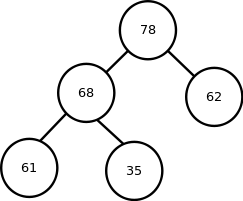
\includegraphics[scale=0.60]{img/binTree}
  \caption{arbre binaire}
  \label{fig:abtree}
\end{figure}
L'arbre binaire était équilibré par définition, la compléxité de son opération de recherche est en $O(log_2 n)$ (hauteur de l'arbre).
   


%http://www.enseignement.polytechnique.fr/profs/informatique/Luc.Maranget/421/poly/arbre-bin.html
\clearpage
\paragraph{Arbres a-b}
Il s'agit d'un arbre de recherche avec les propriétés suivantes :
\begin{itemize}
\item
  $a\leq2$ et $b\leq 2a−1$ deux entiers.
\item
  La racine a au moins 2 fils (sauf si l'arbre ne possède qu'un nœud) et au plus b fils.
  Les feuilles sont de même profondeur.
\item
  Les autres nœuds internes ont au moins a et au plus b fils.
\end{itemize}

\begin{figure}[htbp]
  \centering
  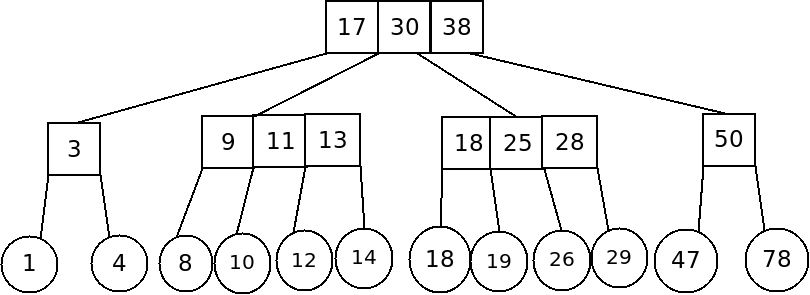
\includegraphics[scale=0.40]{img/abtree}
  \caption{a-b arbre}
  \label{fig:abtree}
\end{figure}

L'avantage des arbres a-b est que leurs hauteurs  sont comprises entres les valeurs suivantes : $ \dfrac{\log{n}}{\log{b}}   \leq h  < 1 + \dfrac{\log{n/2}}{\log{a}}$. Ainsi les opérations d'insertion ne seraient plus en $O(n\log{n})$ mais en $O(\log{n})$. La création d'un pavage composé de $n$ boîtes à $d$ dimensions aurait alors une complexité en $O((n\times d)\log(n))$. La recherche d'un boîte quant à elle aurait une compléxité en $O(\log{n})$.


%\section{Présentation du problème}


\subsection{Données en entrée}
Un problème de satisfaction de contraintes est défini par 3 éléments : 
\begin{itemize}
\item
Un ensemble de variable $\mathbf{V} = \left\{ v_1,...,v_n \right\}$.
\item
Un domaine de valeurs pour chaque variable. Chaque valeur du domaine $D_i$ associé à la variable $v_i$ est une valeur que peut potentiellement prendre $v_i$ : $\mathbf{D} = D_1 \times ... \times D_n $.
\item
Un ensemble de contraintes (relations) $\mathbf{C}$ restreignant les variables de $\mathbf{V}$ défini ci-dessus :  $\mathbf{C} = \left\{c_1,...,cm\right\}$. 
\end{itemize}


\section{Résolution par Intervalles}
Les méthodes formelles et numériques, bien que performantes par certains aspects, sont rapidement limitées lorsque l'on veut résoudre des problèmes complexes ou que l'on veut pouvoir valider une solution (problème de propagation des erreurs\dots). C'est dans ce cadre que la méthode de résolution par intervalles a toute sa places. Construite grâce à l'arithmétique des intervalles, elle utilise aussi des notions apportées par la programmation par contrainte.
 
\subsection{L'Arithmétique des intervalles}
Cette arithmétique permet un calcul sur un ensembles $\mathbb{I}$ d'intervalles sur $\mathbb{R}$. Les bornes $b1$ et $b2$ de l'intervalle $[b1,b2]$, résultant de tout calcul, sont choisies en prenant un arrondi respectivement inférieur à $b1$ et supérieur à $b2$ de manière à garantir l'exactitude des calculs. L'extension des fonctions aux intervalles, introduite par Moore en 1966, permet une transition à des intervalles grâce à un opérateur d'encadrement. Une liste non-exhaustive des opérations de cet opérateur est listée dans \cite{Goualard}.



\subsection{Utilisation des intervalles pour la notion de contraintes}
En utilisant l'arithmétique des intervalles, la méthode de résolution par intervalles utilise des notions de programmation par contraintes. On y retrouve celle de consistance. La consistance consiste à rechercher les valeurs cohérentes dans le domaine des variables pour les contraintes du CSP. Par exemple un CSP est globalement consistant lorsque toutes les valeurs des variables de son domaine appartiennent au moins à une solution. On devine qu'il peut être intéressant pour un CSP de posséder la consistance la plus forte possible. Ainsi les opérations pour la résolution de problèmes seront moins nombreuses.

Dans le cas du problème (\ref{eq}), il serait possible d'avoir des solutions différentes selon la consistance choisie. Avec une hull-consistance, nous obtiendrions une boite contenant les deux solutions mais aussi une bonne partie de l'intersection des deux cercles. Tandis qu'avec une arc-consistance, nous obtiendrions deux boites, plus petites que dans le premier cas, et chacune contenant une des solutions.


\subsection{Exemples d'application}
Les performances de précision de la méthode attirent le monde industriel qui y voit à juste titre, l'occasion de diminuer ses coûts de production par exemple. Par ailleurs, la seule possibilité de trouver un minimum global intéresse régulièrement les industriels. On retrouve en effet dans \cite{Schichl}, le détails d'applications dans le secteur de la chimie industrielle mais aussi dans celui de la biologie avec une étude sur les protéines.
 La science fondamentale met aussi en application ces outils. C'est le cas en mathématique par exemple de problèmes tel que la conjecture de Kepler ou encore le  maximum de clique.

\chapter[B-arbres]{Cas concret : B-arbres%
\chaptermark{B-arbres}}
\section{Définitions}
Un B-arbre est une structure de données en arbre équilibré. Le principe général de cette structure est la minimisation de la taille des arbres en permettant aux noeuds la possession de plusieurs clés. Un B-arbre est donc caractérisé par les propriétés suivantes :
\begin{itemize}
\item Un ordre $m$
\item Chaque noeud contient $k$ clés triées avec :
\begin{itemize}
\item pour le noeud racine : $m \leq k \leq 2m$
\item pour un noeud non racine : $1 \leq k \leq 2m$
\end{itemize}
\item Un noeud est soit :
\begin{itemize}
\item Terminal et donc est une feuille.
\item Non terminal et possède alors $k+1$ fils. Les clés du $i$\up{ème} fils ont des valeurs comprises entre les valeurs des $(i-1)$\up{ème} et $i$\up{ème} clés du père.
\end{itemize}
\item Chaque chemin de la racine à une feuille est de même longueur $h$ (hauteur).
\end{itemize}

\begin{figure}[h]
	\centering
	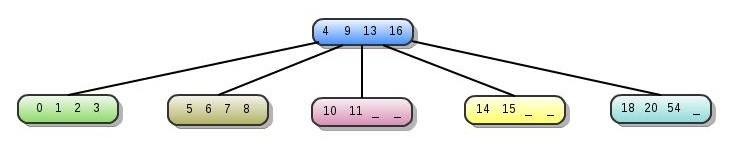
\includegraphics[scale=0.5]{barbre}
	\caption{Exemple de B-arbre}
	\label{fig:barbre}
\end{figure}

Étant donné la forme dont sont stockées les données dans les B-arbres (tri) et l'exécution des opérations d'insertion et de suppression en temps amorti logarithmique, cette structure est principalement mise en œuvre dans les mécanismes de gestion des bases de données et des systèmes de fichiers.
\section{Implémentations}
\subsection{Méthodologie et choix de structure}
En considérant les propriétés des B-arbres décrites précédemment, nous avons procédé dans la construction de nos structures/algorithmes de la manière suivante : 
\begin{enumerate}
\item Mise en place de classes génériques en utilisant le principe des “templates”: L’objectif de cette approche est de générer le code spécifique à chaque type à partir d'un modèle générique. L’intérêt de cette technique est double : nous disposons d’un code optimisé pour chaque type et le code source n'est pas dupliqué car il écrit un méta-code à partir duquel sont générés les codes spécifiques. Nous avons donc paramétré nos arbres par le type de données à stocker et nous avons choisi de fixer l’ordre du B-Arbre.
\begin{lstlisting}
//T un type quelconque et k l ordre de l arbre
template<class T,short k>
\end{lstlisting}
\item     Mise en place de la structure de noeud "\verb+BTreeItem+": Cette structure comporte les éléments suivants :
\begin{itemize}
\item     Deux variables \verb+k+ et \verb+nCount+ de types entier court représentant respectivement l'ordre de l'arbre et le nombre de clés stockés dans un noeud.
\item     Un tableau \verb+data+ de $2 \times k$ clés rangées dans l'ordre croissant.
\item     Un tableau \verb+subItems+ de $2\times k+1$ pointeurs vers les enfants du noeud lorsque celui-ci n'est pas une feuille.
\end{itemize}
Cette structure possède également deux fonctions qui nous serviront dans la méthode d’insertion dans le B-arbre :
\begin{itemize}
\item     Une fonction de recherche dichotomique\cite{dichotomie} \verb+searchInNode+.
\item         Une fonction de "découpage" de noeud \verb+SplitNode+.   
\end{itemize}
\item     Mise en place de la structure d’arbre complète \verb+BTree+ : cette structure comporte les fonctions nécessaires pour la recherche d’un élément dans l’arbre, la suppression ainsi que l’ajout. Nous verrons ces fonctionnalités plus en détails dans les parties qui suivent.
\end{enumerate}

\subsection{Méthode de recherche}
La recherche est effectuée de la même manière que dans un arbre binaire de recherche, d'où l'utilisation de la fonction de recherche dichotomique citée précedemment. Partant de la racine, nous parcourons récursivement l’arbre. À chaque nœud, nous choisissons le sous-arbre fils dont les clés sont comprises entre les mêmes bornes que celles de la clé recherchée.
\paragraph{Algorithme} Nous avons la structure de noeud suivante :
\begin{figure}[hbt]
	\centering
	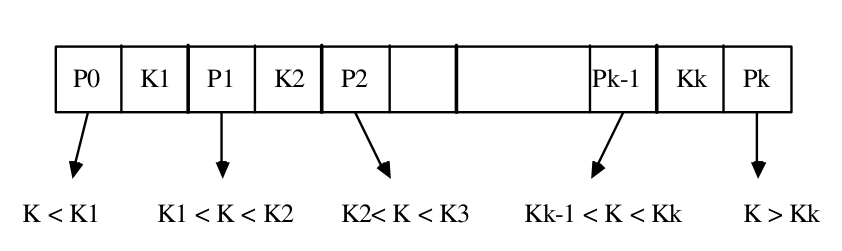
\includegraphics[scale=0.5]{node}
	\caption{Représentation de la structure}
	\label{fig:node}
\end{figure}

avec $K_1 < K_2 < K_3 < \dots < K_n$ clés et $P_0$,...,$P_k$ pointeurs vers noeuds enfants.

Pour chercher une clé $k$ dans le B-arbre, l'algorithme récursif a été imaginé à partir des grandes étapes suivantes : 

A partir de la racine et pour chaque noeud, on examine :
\begin{itemize}
\item \emph{si la clé est présente} \\ succès
\item \emph{si $K<K_1$} \\recherche dans $P_0$
\item \emph{si $K>K_n$}\\ recherche dans $P_k$
\item \emph{si $K_i < k < K_{i+1}$}\\ recherche dans $P_i$
\end{itemize}

\subsection{Méthode d’insertion}
L’insertion se déroule globalement de la manière suivante :
\begin{itemize}
\item Recherche de la feuille d’insertion
\item Si la feuille n’est pas pleine
\begin{itemize}
\item Alors insérer la feuille à sa place
\end{itemize}
\item Sinon (la feuille est pleine: $2 \times k$ clés)
\begin{itemize}
\item Laisser les $k$ plus petites clés dans le noeud
\item Allouer un nouveau noeud et y placer les k plus grandes clés
\item Remonter la clé médiane au noeud père
\end{itemize}
\end{itemize}

\appendix
\chapter{Sortie RealPaver : intersection de deux disques}\label{chap:realout}
\begin{verbatim}

RealPaver v. 0.4 (c) LINA 2004

INITIAL BOX
  x in ]-oo , +oo[
  y in ]-oo , +oo[

INNER BOX 1
  x in [-0.3333333333333334 , +0.3333333333333333]
  y in [-0.6666666666666667 , +0.6666666666666665]

  precision: 1.33, elapsed time: 0 ms

INNER BOX 2
  x in [-0.2952060277213756 , +0.2952060277213757]
  y in [-1.470023035500388 , -1.068344851083527]

  precision: 0.59, elapsed time: 0 ms

INNER BOX 3
  x in [-0.2952060277213756 , +0.2952060277213757]
  y in [-1.068344851083527 , -0.6666666666666667]

  precision: 0.59, elapsed time: 0 ms

INNER BOX 4
  x in [-0.2952060277213756 , +0.2952060277213757]
  y in [0.6666666666666665 , 1.068344851083527]

  precision: 0.59, elapsed time: 0 ms

INNER BOX 5
  x in [-0.2952060277213756 , +0.2952060277213757]
  y in [1.068344851083527 , 1.470023035500388]

  precision: 0.59, elapsed time: 0 ms

INNER BOX 6
  x in [-0.4496899872832925 , -0.2952060277213756]
  y in [-1.238192769860558 , -0.9524297182636126]

  precision: 0.286, elapsed time: 0 ms

INNER BOX 7
  x in [-0.6888140646832098 , -0.4920100462022927]
  y in [-0.9524297182636126 , -0.6666666666666667]

  precision: 0.286, elapsed time: 0 ms

INNER BOX 8
  x in [-0.4920100462022927 , -0.2952060277213756]
  y in [-0.9524297182636126 , -0.6666666666666667]

  precision: 0.286, elapsed time: 0 ms

INNER BOX 9
  x in [0.2952060277213757 , 0.4496899872832926]
  y in [-1.238192769860558 , -0.9524297182636123]

  precision: 0.286, elapsed time: 0 ms

INNER BOX 10
  x in [0.2952060277213757 , 0.4920100462022928]
  y in [-0.9524297182636123 , -0.6666666666666667]

  precision: 0.286, elapsed time: 0 ms

INNER BOX 11
  x in [0.4920100462022928 , 0.6888140646832099]
  y in [-0.9524297182636123 , -0.6666666666666667]

  precision: 0.286, elapsed time: 0 ms

INNER BOX 12
  x in [-0.7695217644443199 , -0.5514275488888266]
  y in [-0.6666666666666667 , -0.2222222222222223]

  precision: 0.444, elapsed time: 0 ms

INNER BOX 13
  x in [-0.5514275488888266 , -0.3333333333333334]
  y in [-0.6666666666666667 , -0.2222222222222223]

  precision: 0.444, elapsed time: 0 ms

INNER BOX 14
  x in [-0.7777777777777778 , -0.5555555555555556]
  y in [-0.2222222222222223 , +0.2222222222222221]

  precision: 0.444, elapsed time: 0 ms

INNER BOX 15
  x in [-0.5555555555555556 , -0.3333333333333334]
  y in [-0.2222222222222223 , +0.2222222222222221]

  precision: 0.444, elapsed time: 0 ms

INNER BOX 16
  x in [-0.7695217644443199 , -0.5514275488888266]
  y in [0.2222222222222221 , 0.6666666666666665]

  precision: 0.444, elapsed time: 0 ms

INNER BOX 17
  x in [-0.5514275488888266 , -0.3333333333333334]
  y in [0.2222222222222221 , 0.6666666666666665]

  precision: 0.444, elapsed time: 0 ms

INNER BOX 18
  x in [0.3333333333333333 , 0.5514275488888266]
  y in [-0.6666666666666667 , -0.2222222222222223]

  precision: 0.444, elapsed time: 0 ms

INNER BOX 19
  x in [0.5514275488888266 , 0.76952176444432]
  y in [-0.6666666666666667 , -0.2222222222222223]

  precision: 0.444, elapsed time: 0 ms

INNER BOX 20
  x in [0.3333333333333333 , 0.5555555555555556]
  y in [-0.2222222222222223 , +0.2222222222222221]

  precision: 0.444, elapsed time: 0 ms

INNER BOX 21
  x in [0.5555555555555556 , 0.7777777777777778]
  y in [-0.2222222222222223 , +0.2222222222222221]

  precision: 0.444, elapsed time: 0 ms

INNER BOX 22
  x in [0.3333333333333333 , 0.5514275488888266]
  y in [0.2222222222222221 , 0.6666666666666665]

  precision: 0.444, elapsed time: 0 ms

INNER BOX 23
  x in [0.5514275488888266 , 0.76952176444432]
  y in [0.2222222222222221 , 0.6666666666666665]

  precision: 0.444, elapsed time: 0 ms

INNER BOX 24
  x in [-0.6888140646832098 , -0.4920100462022927]
  y in [0.6666666666666665 , 0.9524297182636124]

  precision: 0.286, elapsed time: 0 ms

INNER BOX 25
  x in [-0.4920100462022927 , -0.2952060277213756]
  y in [0.6666666666666665 , 0.9524297182636124]

  precision: 0.286, elapsed time: 0 ms

INNER BOX 26
  x in [-0.4496899872832925 , -0.2952060277213756]
  y in [0.9524297182636124 , 1.238192769860558]

  precision: 0.286, elapsed time: 0 ms

INNER BOX 27
  x in [0.2952060277213757 , 0.4920100462022928]
  y in [0.6666666666666665 , 0.9524297182636123]

  precision: 0.286, elapsed time: 0 ms

INNER BOX 28
  x in [0.4920100462022928 , 0.6888140646832099]
  y in [0.6666666666666665 , 0.9524297182636123]

  precision: 0.286, elapsed time: 0 ms

INNER BOX 29
  x in [0.2952060277213757 , 0.4496899872832926]
  y in [0.9524297182636123 , 1.238192769860558]

  precision: 0.286, elapsed time: 0 ms

INNER BOX 30
  x in [-0.3603407527950472 , -0.2952060277213756]
  y in [-1.428701470925189 , -1.333447120392873]

  precision: 0.0953, elapsed time: 0 ms

INNER BOX 31
  x in [-0.4788220236221691 , -0.3870140256717723]
  y in [-1.333447120392873 , -1.238192769860558]

  precision: 0.0953, elapsed time: 0 ms

INNER BOX 32
  x in [-0.3870140256717723 , -0.2952060277213756]
  y in [-1.333447120392873 , -1.238192769860558]

  precision: 0.0953, elapsed time: 0 ms

INNER BOX 33
  x in [-0.6041739468452093 , -0.4496899872832925]
  y in [-1.142938419328243 , -1.047684068795928]

  precision: 0.154, elapsed time: 0 ms

INNER BOX 34
  x in [-0.6041739468452093 , -0.4496899872832925]
  y in [-1.047684068795928 , -0.9524297182636126]

  precision: 0.154, elapsed time: 0 ms

INNER BOX 35
  x in [-0.0984020092404585 , +0.09840200924045861]
  y in [-1.575099017137251 , -1.470023035500388]

  precision: 0.197, elapsed time: 0 ms

INNER BOX 36
  x in [0.2952060277213757 , 0.3603407527950474]
  y in [-1.428701470925188 , -1.333447120392873]

  precision: 0.0953, elapsed time: 0 ms

INNER BOX 37
  x in [0.2952060277213757 , 0.3870140256717726]
  y in [-1.333447120392873 , -1.238192769860558]

  precision: 0.0953, elapsed time: 0 ms

INNER BOX 38
  x in [0.3870140256717726 , 0.4788220236221695]
  y in [-1.333447120392873 , -1.238192769860558]

  precision: 0.0953, elapsed time: 0 ms

INNER BOX 39
  x in [0.4496899872832926 , 0.6041739468452095]
  y in [-1.142938419328243 , -1.047684068795927]

  precision: 0.154, elapsed time: 0 ms

INNER BOX 40
  x in [0.4496899872832926 , 0.6041739468452095]
  y in [-1.047684068795927 , -0.9524297182636123]

  precision: 0.154, elapsed time: 0 ms

INNER BOX 41
  x in [-0.6041739468452093 , -0.4496899872832925]
  y in [0.9524297182636124 , 1.047684068795928]

  precision: 0.154, elapsed time: 0 ms

INNER BOX 42
  x in [-0.6041739468452093 , -0.4496899872832925]
  y in [1.047684068795928 , 1.142938419328243]

  precision: 0.154, elapsed time: 0 ms

INNER BOX 43
  x in [-0.4788220236221691 , -0.3870140256717723]
  y in [1.238192769860558 , 1.333447120392874]

  precision: 0.0953, elapsed time: 0 ms

INNER BOX 44
  x in [-0.3870140256717723 , -0.2952060277213756]
  y in [1.238192769860558 , 1.333447120392874]

  precision: 0.0953, elapsed time: 0 ms

INNER BOX 45
  x in [-0.3603407527950471 , -0.2952060277213756]
  y in [1.333447120392874 , 1.428701470925189]

  precision: 0.0953, elapsed time: 0 ms

INNER BOX 46
  x in [-0.0984020092404585 , +0.09840200924045861]
  y in [1.470023035500388 , 1.575099017137252]

  precision: 0.197, elapsed time: 0 ms

INNER BOX 47
  x in [0.4496899872832926 , 0.6041739468452095]
  y in [0.9524297182636123 , 1.047684068795928]

  precision: 0.154, elapsed time: 0 ms

INNER BOX 48
  x in [0.4496899872832926 , 0.6041739468452095]
  y in [1.047684068795928 , 1.142938419328243]

  precision: 0.154, elapsed time: 0 ms

INNER BOX 49
  x in [0.2952060277213757 , 0.3870140256717726]
  y in [1.238192769860558 , 1.333447120392873]

  precision: 0.0953, elapsed time: 0 ms

INNER BOX 50
  x in [0.3870140256717726 , 0.4788220236221694]
  y in [1.238192769860558 , 1.333447120392873]

  precision: 0.0953, elapsed time: 0 ms

INNER BOX 51
  x in [0.2952060277213757 , 0.3603407527950473]
  y in [1.333447120392873 , 1.428701470925189]

  precision: 0.0953, elapsed time: 0 ms

INNER BOX 52
  x in [-0.3647858013680041 , -0.3299959145446899]
  y in [-1.450364431242905 , -1.428701470925189]

  precision: 0.0348, elapsed time: 0 ms

INNER BOX 53
  x in [-0.3299959145446899 , -0.2952060277213756]
  y in [-1.492204371280066 , -1.460452921102627]

  precision: 0.0348, elapsed time: 0 ms

INNER BOX 54
  x in [-0.3299959145446899 , -0.2952060277213756]
  y in [-1.460452921102627 , -1.428701470925189]

  precision: 0.0348, elapsed time: 0 ms

INNER BOX 55
  x in [-0.4254754778687188 , -0.3603407527950472]
  y in [-1.39695002074775 , -1.365198570570312]

  precision: 0.0651, elapsed time: 0 ms

INNER BOX 56
  x in [-0.4254754778687188 , -0.3603407527950472]
  y in [-1.365198570570312 , -1.333447120392873]

  precision: 0.0651, elapsed time: 0 ms

INNER BOX 57
  x in [-0.640289064769753 , -0.6041739468452093]
  y in [-1.113752892260402 , -1.033091305262007]

  precision: 0.0807, elapsed time: 0 ms

INNER BOX 58
  x in [-0.7071632532198205 , -0.6556686000325149]
  y in [-1.033091305262007 , -0.9524297182636126]

  precision: 0.0807, elapsed time: 0 ms

INNER BOX 59
  x in [-0.6556686000325149 , -0.6041739468452093]
  y in [-1.033091305262007 , -0.9524297182636126]

  precision: 0.0807, elapsed time: 0 ms

INNER BOX 60
  x in [-0.5526792936579037 , -0.5011846404705981]
  y in [-1.238192769860558 , -1.142938419328243]

  precision: 0.0953, elapsed time: 0 ms

INNER BOX 61
  x in [-0.5011846404705981 , -0.4496899872832925]
  y in [-1.238192769860558 , -1.142938419328243]

  precision: 0.0953, elapsed time: 0 ms

INNER BOX 62
  x in [-0.7282095045641771 , -0.6888140646832098]
  y in [-0.9524297182636126 , -0.8571753677312972]

  precision: 0.0953, elapsed time: 0 ms

INNER BOX 63
  x in [-0.7957264351540503 , -0.74227024991863]
  y in [-0.8571753677312972 , -0.761921017198982]

  precision: 0.0953, elapsed time: 0 ms

INNER BOX 64
  x in [-0.74227024991863 , -0.6888140646832098]
  y in [-0.8571753677312972 , -0.761921017198982]

  precision: 0.0953, elapsed time: 0 ms

INNER BOX 65
  x in [-0.8200167436704878 , -0.7544154041768488]
  y in [-0.761921017198982 , -0.6666666666666667]

  precision: 0.0953, elapsed time: 0 ms

INNER BOX 66
  x in [-0.7544154041768488 , -0.6888140646832098]
  y in [-0.761921017198982 , -0.6666666666666667]

  precision: 0.0953, elapsed time: 0 ms

INNER BOX 67
  x in [-0.1587775879152689 , -0.0984020092404585]
  y in [-1.604261395088855 , -1.537142215294622]

  precision: 0.0671, elapsed time: 0 ms

INNER BOX 68
  x in [-0.2296046882277366 , -0.1640033487340975]
  y in [-1.537142215294622 , -1.470023035500388]

  precision: 0.0671, elapsed time: 0 ms

INNER BOX 69
  x in [-0.1640033487340975 , -0.0984020092404585]
  y in [-1.537142215294622 , -1.470023035500388]

  precision: 0.0671, elapsed time: 0 ms

INNER BOX 70
  x in [-0.03280066974681946 , +0.03280066974681958]
  y in [-1.680174998774115 , -1.575099017137251]

  precision: 0.105, elapsed time: 0 ms

INNER BOX 71
  x in [0.09840200924045861 , 0.158777587915269]
  y in [-1.604261395088855 , -1.537142215294622]

  precision: 0.0671, elapsed time: 0 ms

INNER BOX 72
  x in [0.09840200924045861 , 0.1640033487340977]
  y in [-1.537142215294622 , -1.470023035500388]

  precision: 0.0671, elapsed time: 0 ms

INNER BOX 73
  x in [0.1640033487340977 , 0.2296046882277367]
  y in [-1.537142215294622 , -1.470023035500388]

  precision: 0.0671, elapsed time: 0 ms

INNER BOX 74
  x in [0.2952060277213757 , 0.3299959145446901]
  y in [-1.492204371280065 , -1.460452921102627]

  precision: 0.0348, elapsed time: 0 ms

INNER BOX 75
  x in [0.2952060277213757 , 0.3299959145446901]
  y in [-1.460452921102627 , -1.428701470925188]

  precision: 0.0348, elapsed time: 0 ms

INNER BOX 76
  x in [0.3299959145446901 , 0.3647858013680045]
  y in [-1.450364431242905 , -1.428701470925188]

  precision: 0.0348, elapsed time: 0 ms

INNER BOX 77
  x in [0.3603407527950474 , 0.425475477868719]
  y in [-1.39695002074775 , -1.365198570570311]

  precision: 0.0651, elapsed time: 0 ms

INNER BOX 78
  x in [0.3603407527950474 , 0.425475477868719]
  y in [-1.365198570570311 , -1.333447120392873]

  precision: 0.0651, elapsed time: 0 ms

INNER BOX 79
  x in [0.4496899872832926 , 0.5011846404705983]
  y in [-1.238192769860558 , -1.142938419328243]

  precision: 0.0953, elapsed time: 0 ms

INNER BOX 80
  x in [0.5011846404705983 , 0.5526792936579039]
  y in [-1.238192769860558 , -1.142938419328243]

  precision: 0.0953, elapsed time: 0 ms

INNER BOX 81
  x in [0.6041739468452095 , 0.6402890647697532]
  y in [-1.113752892260402 , -1.033091305262007]

  precision: 0.0807, elapsed time: 0 ms

INNER BOX 82
  x in [0.6041739468452095 , 0.6556686000325151]
  y in [-1.033091305262007 , -0.9524297182636123]

  precision: 0.0807, elapsed time: 0 ms

INNER BOX 83
  x in [0.6556686000325151 , 0.7071632532198208]
  y in [-1.033091305262007 , -0.9524297182636123]

  precision: 0.0807, elapsed time: 0 ms

INNER BOX 84
  x in [0.6888140646832099 , 0.7282095045641773]
  y in [-0.9524297182636123 , -0.8571753677312971]

  precision: 0.0953, elapsed time: 0 ms

INNER BOX 85
  x in [0.6888140646832099 , 0.7422702499186302]
  y in [-0.8571753677312971 , -0.7619210171989819]

  precision: 0.0953, elapsed time: 0 ms

INNER BOX 86
  x in [0.7422702499186302 , 0.7957264351540504]
  y in [-0.8571753677312971 , -0.7619210171989819]

  precision: 0.0953, elapsed time: 0 ms

INNER BOX 87
  x in [0.6888140646832099 , 0.7544154041768489]
  y in [-0.7619210171989819 , -0.6666666666666667]

  precision: 0.0953, elapsed time: 0 ms

INNER BOX 88
  x in [0.7544154041768489 , 0.8200167436704879]
  y in [-0.7619210171989819 , -0.6666666666666667]

  precision: 0.0953, elapsed time: 0 ms

INNER BOX 89
  x in [-0.8775842731264076 , -0.8235530187853637]
  y in [-0.6666666666666667 , -0.5185185185185186]

  precision: 0.148, elapsed time: 0 ms

INNER BOX 90
  x in [-0.8235530187853637 , -0.7695217644443199]
  y in [-0.6666666666666667 , -0.5185185185185186]

  precision: 0.148, elapsed time: 0 ms

INNER BOX 91
  x in [-0.9001121102638202 , -0.83481693735407]
  y in [-0.5185185185185186 , -0.3703703703703705]

  precision: 0.148, elapsed time: 0 ms

INNER BOX 92
  x in [-0.83481693735407 , -0.7695217644443199]
  y in [-0.5185185185185186 , -0.3703703703703705]

  precision: 0.148, elapsed time: 0 ms

INNER BOX 93
  x in [-0.914917908147982 , -0.8422198362961509]
  y in [-0.3703703703703705 , -0.2222222222222223]

  precision: 0.148, elapsed time: 0 ms

INNER BOX 94
  x in [-0.8422198362961509 , -0.7695217644443199]
  y in [-0.3703703703703705 , -0.2222222222222223]

  precision: 0.148, elapsed time: 0 ms

INNER BOX 95
  x in [-0.9250111173562511 , -0.8513944475670144]
  y in [-0.2222222222222223 , -0.07407407407407418]

  precision: 0.148, elapsed time: 0 ms

INNER BOX 96
  x in [-0.8513944475670144 , -0.7777777777777778]
  y in [-0.2222222222222223 , -0.07407407407407418]

  precision: 0.148, elapsed time: 0 ms

INNER BOX 97
  x in [-0.9259259259259259 , -0.8518518518518519]
  y in [-0.07407407407407418 , +0.07407407407407396]

  precision: 0.148, elapsed time: 0 ms

INNER BOX 98
  x in [-0.8518518518518519 , -0.7777777777777778]
  y in [-0.07407407407407418 , +0.07407407407407396]

  precision: 0.148, elapsed time: 0 ms

INNER BOX 99
  x in [-0.9250111173562511 , -0.8513944475670144]
  y in [0.07407407407407396 , 0.2222222222222221]

  precision: 0.148, elapsed time: 0 ms

INNER BOX 100
  x in [-0.8513944475670144 , -0.7777777777777778]
  y in [0.07407407407407396 , 0.2222222222222221]

  precision: 0.148, elapsed time: 0 ms

INNER BOX 101
  x in [-0.914917908147982 , -0.8422198362961509]
  y in [0.2222222222222221 , 0.3703703703703702]

  precision: 0.148, elapsed time: 0 ms

INNER BOX 102
  x in [-0.8422198362961509 , -0.7695217644443199]
  y in [0.2222222222222221 , 0.3703703703703702]

  precision: 0.148, elapsed time: 0 ms

INNER BOX 103
  x in [-0.9001121102638202 , -0.83481693735407]
  y in [0.3703703703703702 , 0.5185185185185184]

  precision: 0.148, elapsed time: 0 ms

INNER BOX 104
  x in [-0.83481693735407 , -0.7695217644443199]
  y in [0.3703703703703702 , 0.5185185185185184]

  precision: 0.148, elapsed time: 0 ms

INNER BOX 105
  x in [-0.8775842731264077 , -0.8235530187853638]
  y in [0.5185185185185184 , 0.6666666666666665]

  precision: 0.148, elapsed time: 0 ms

INNER BOX 106
  x in [-0.8235530187853638 , -0.7695217644443199]
  y in [0.5185185185185184 , 0.6666666666666665]

  precision: 0.148, elapsed time: 0 ms

INNER BOX 107
  x in [0.76952176444432 , 0.8235530187853639]
  y in [-0.6666666666666667 , -0.5185185185185186]

  precision: 0.148, elapsed time: 0 ms

INNER BOX 108
  x in [0.8235530187853639 , 0.8775842731264077]
  y in [-0.6666666666666667 , -0.5185185185185186]

  precision: 0.148, elapsed time: 0 ms

INNER BOX 109
  x in [0.76952176444432 , 0.8348169373540701]
  y in [-0.5185185185185186 , -0.3703703703703705]

  precision: 0.148, elapsed time: 0 ms

INNER BOX 110
  x in [0.8348169373540701 , 0.9001121102638203]
  y in [-0.5185185185185186 , -0.3703703703703705]

  precision: 0.148, elapsed time: 0 ms

INNER BOX 111
  x in [0.76952176444432 , 0.842219836296151]
  y in [-0.3703703703703705 , -0.2222222222222223]

  precision: 0.148, elapsed time: 0 ms

INNER BOX 112
  x in [0.842219836296151 , 0.9149179081479821]
  y in [-0.3703703703703705 , -0.2222222222222223]

  precision: 0.148, elapsed time: 0 ms

INNER BOX 113
  x in [0.7777777777777778 , 0.8513944475670145]
  y in [-0.2222222222222223 , -0.07407407407407418]

  precision: 0.148, elapsed time: 0 ms

INNER BOX 114
  x in [0.8513944475670145 , 0.9250111173562512]
  y in [-0.2222222222222223 , -0.07407407407407418]

  precision: 0.148, elapsed time: 0 ms

INNER BOX 115
  x in [0.7777777777777778 , 0.8518518518518519]
  y in [-0.07407407407407418 , +0.07407407407407396]

  precision: 0.148, elapsed time: 0 ms

INNER BOX 116
  x in [0.8518518518518519 , 0.9259259259259259]
  y in [-0.07407407407407418 , +0.07407407407407396]

  precision: 0.148, elapsed time: 0 ms

INNER BOX 117
  x in [0.7777777777777778 , 0.8513944475670145]
  y in [0.07407407407407396 , 0.2222222222222221]

  precision: 0.148, elapsed time: 0 ms

INNER BOX 118
  x in [0.8513944475670145 , 0.9250111173562512]
  y in [0.07407407407407396 , 0.2222222222222221]

  precision: 0.148, elapsed time: 0 ms

INNER BOX 119
  x in [0.76952176444432 , 0.842219836296151]
  y in [0.2222222222222221 , 0.3703703703703702]

  precision: 0.148, elapsed time: 0 ms

INNER BOX 120
  x in [0.842219836296151 , 0.9149179081479821]
  y in [0.2222222222222221 , 0.3703703703703702]

  precision: 0.148, elapsed time: 0 ms

INNER BOX 121
  x in [0.76952176444432 , 0.8348169373540701]
  y in [0.3703703703703702 , 0.5185185185185184]

  precision: 0.148, elapsed time: 0 ms

INNER BOX 122
  x in [0.8348169373540701 , 0.9001121102638203]
  y in [0.3703703703703702 , 0.5185185185185184]

  precision: 0.148, elapsed time: 0 ms

INNER BOX 123
  x in [0.76952176444432 , 0.8235530187853639]
  y in [0.5185185185185184 , 0.6666666666666665]

  precision: 0.148, elapsed time: 0 ms

INNER BOX 124
  x in [0.8235530187853639 , 0.8775842731264079]
  y in [0.5185185185185184 , 0.6666666666666665]

  precision: 0.148, elapsed time: 0 ms

INNER BOX 125
  x in [-0.8200167436704878 , -0.7544154041768488]
  y in [0.6666666666666665 , 0.7619210171989819]

  precision: 0.0953, elapsed time: 0 ms

INNER BOX 126
  x in [-0.7544154041768488 , -0.6888140646832098]
  y in [0.6666666666666665 , 0.7619210171989819]

  precision: 0.0953, elapsed time: 0 ms

INNER BOX 127
  x in [-0.7957264351540503 , -0.74227024991863]
  y in [0.7619210171989819 , 0.8571753677312972]

  precision: 0.0953, elapsed time: 0 ms

INNER BOX 128
  x in [-0.74227024991863 , -0.6888140646832098]
  y in [0.7619210171989819 , 0.8571753677312972]

  precision: 0.0953, elapsed time: 0 ms

INNER BOX 129
  x in [-0.7282095045641771 , -0.6888140646832098]
  y in [0.8571753677312972 , 0.9524297182636124]

  precision: 0.0953, elapsed time: 0 ms

INNER BOX 130
  x in [-0.7071632532198205 , -0.6556686000325149]
  y in [0.9524297182636124 , 1.033091305262007]

  precision: 0.0807, elapsed time: 0 ms

INNER BOX 131
  x in [-0.6556686000325149 , -0.6041739468452093]
  y in [0.9524297182636124 , 1.033091305262007]

  precision: 0.0807, elapsed time: 0 ms

INNER BOX 132
  x in [-0.640289064769753 , -0.6041739468452093]
  y in [1.033091305262007 , 1.113752892260403]

  precision: 0.0807, elapsed time: 0 ms

INNER BOX 133
  x in [-0.5526792936579037 , -0.5011846404705981]
  y in [1.142938419328243 , 1.238192769860558]

  precision: 0.0953, elapsed time: 0 ms

INNER BOX 134
  x in [-0.5011846404705981 , -0.4496899872832925]
  y in [1.142938419328243 , 1.238192769860558]

  precision: 0.0953, elapsed time: 0 ms

INNER BOX 135
  x in [-0.4254754778687185 , -0.3603407527950471]
  y in [1.333447120392874 , 1.365198570570312]

  precision: 0.0651, elapsed time: 0 ms

INNER BOX 136
  x in [-0.4254754778687185 , -0.3603407527950471]
  y in [1.365198570570312 , 1.396950020747751]

  precision: 0.0651, elapsed time: 0 ms

INNER BOX 137
  x in [-0.3647858013680038 , -0.3299959145446897]
  y in [1.428701470925189 , 1.450364431242906]

  precision: 0.0348, elapsed time: 0 ms

INNER BOX 138
  x in [-0.3299959145446897 , -0.2952060277213756]
  y in [1.428701470925189 , 1.460452921102628]

  precision: 0.0348, elapsed time: 0 ms

INNER BOX 139
  x in [-0.3299959145446897 , -0.2952060277213756]
  y in [1.460452921102628 , 1.492204371280066]

  precision: 0.0348, elapsed time: 0 ms

INNER BOX 140
  x in [-0.2296046882277366 , -0.1640033487340975]
  y in [1.470023035500388 , 1.537142215294622]

  precision: 0.0671, elapsed time: 0 ms

INNER BOX 141
  x in [-0.1640033487340975 , -0.0984020092404585]
  y in [1.470023035500388 , 1.537142215294622]

  precision: 0.0671, elapsed time: 0 ms

INNER BOX 142
  x in [-0.1587775879152689 , -0.0984020092404585]
  y in [1.537142215294622 , 1.604261395088855]

  precision: 0.0671, elapsed time: 0 ms

INNER BOX 143
  x in [-0.03280066974681946 , +0.03280066974681958]
  y in [1.575099017137252 , 1.680174998774115]

  precision: 0.105, elapsed time: 0 ms

INNER BOX 144
  x in [0.09840200924045861 , 0.1640033487340977]
  y in [1.470023035500388 , 1.537142215294622]

  precision: 0.0671, elapsed time: 0 ms

INNER BOX 145
  x in [0.1640033487340977 , 0.2296046882277367]
  y in [1.470023035500388 , 1.537142215294622]

  precision: 0.0671, elapsed time: 0 ms

INNER BOX 146
  x in [0.09840200924045861 , 0.1587775879152689]
  y in [1.537142215294622 , 1.604261395088855]

  precision: 0.0671, elapsed time: 0 ms

INNER BOX 147
  x in [0.6888140646832099 , 0.7544154041768489]
  y in [0.6666666666666665 , 0.7619210171989819]

  precision: 0.0953, elapsed time: 0 ms

INNER BOX 148
  x in [0.7544154041768489 , 0.8200167436704879]
  y in [0.6666666666666665 , 0.7619210171989819]

  precision: 0.0953, elapsed time: 0 ms

INNER BOX 149
  x in [0.6888140646832099 , 0.7422702499186302]
  y in [0.7619210171989819 , 0.8571753677312971]

  precision: 0.0953, elapsed time: 0 ms

INNER BOX 150
  x in [0.7422702499186302 , 0.7957264351540504]
  y in [0.7619210171989819 , 0.8571753677312971]

  precision: 0.0953, elapsed time: 0 ms

INNER BOX 151
  x in [0.6888140646832099 , 0.7282095045641773]
  y in [0.8571753677312971 , 0.9524297182636123]

  precision: 0.0953, elapsed time: 0 ms

INNER BOX 152
  x in [0.4496899872832926 , 0.5011846404705983]
  y in [1.142938419328243 , 1.238192769860558]

  precision: 0.0953, elapsed time: 0 ms

INNER BOX 153
  x in [0.5011846404705983 , 0.5526792936579039]
  y in [1.142938419328243 , 1.238192769860558]

  precision: 0.0953, elapsed time: 0 ms

INNER BOX 154
  x in [0.6041739468452095 , 0.6556686000325151]
  y in [0.9524297182636123 , 1.033091305262007]

  precision: 0.0807, elapsed time: 0 ms

INNER BOX 155
  x in [0.6556686000325151 , 0.7071632532198208]
  y in [0.9524297182636123 , 1.033091305262007]

  precision: 0.0807, elapsed time: 0 ms

INNER BOX 156
  x in [0.6041739468452095 , 0.6402890647697532]
  y in [1.033091305262007 , 1.113752892260403]

  precision: 0.0807, elapsed time: 0 ms

INNER BOX 157
  x in [0.3603407527950473 , 0.4254754778687189]
  y in [1.333447120392873 , 1.365198570570312]

  precision: 0.0651, elapsed time: 0 ms

INNER BOX 158
  x in [0.3603407527950473 , 0.4254754778687189]
  y in [1.365198570570312 , 1.39695002074775]

  precision: 0.0651, elapsed time: 0 ms

INNER BOX 159
  x in [0.2952060277213757 , 0.32999591454469]
  y in [1.428701470925189 , 1.460452921102627]

  precision: 0.0348, elapsed time: 0 ms

INNER BOX 160
  x in [0.2952060277213757 , 0.32999591454469]
  y in [1.460452921102627 , 1.492204371280065]

  precision: 0.0348, elapsed time: 0 ms

INNER BOX 161
  x in [0.32999591454469 , 0.3647858013680043]
  y in [1.428701470925189 , 1.450364431242905]

  precision: 0.0348, elapsed time: 0 ms

INNER BOX 162
  x in [-0.3879790592502136 , -0.3763824303091088]
  y in [-1.436153886898494 , -1.428701470925189]

  precision: 0.0116, elapsed time: 0 ms

INNER BOX 163
  x in [-0.3763824303091088 , -0.3647858013680041]
  y in [-1.450881273608308 , -1.439791372266748]

  precision: 0.0116, elapsed time: 0 ms

INNER BOX 164
  x in [-0.3763824303091088 , -0.3647858013680041]
  y in [-1.439791372266748 , -1.428701470925189]

  precision: 0.0116, elapsed time: 0 ms

INNER BOX 165
  x in [-0.3531891724268993 , -0.3415925434857946]
  y in [-1.472027391560622 , -1.450364431242905]

  precision: 0.0217, elapsed time: 0 ms

INNER BOX 166
  x in [-0.3415925434857946 , -0.3299959145446899]
  y in [-1.472027391560622 , -1.450364431242905]

  precision: 0.0217, elapsed time: 0 ms

INNER BOX 167
  x in [-0.4401782696806391 , -0.4254754778687188]
  y in [-1.379723200915215 , -1.356585160654044]

  precision: 0.0231, elapsed time: 0 ms

INNER BOX 168
  x in [-0.4688986279178332 , -0.447187052893276]
  y in [-1.356585160654044 , -1.333447120392873]

  precision: 0.0231, elapsed time: 0 ms

INNER BOX 169
  x in [-0.447187052893276 , -0.4254754778687188]
  y in [-1.356585160654044 , -1.333447120392873]

  precision: 0.0231, elapsed time: 0 ms

INNER BOX 170
  x in [-0.3820523278196044 , -0.3603407527950472]
  y in [-1.428701470925189 , -1.39695002074775]

  precision: 0.0318, elapsed time: 0 ms

INNER BOX 171
  x in [-0.5009047226602127 , -0.4788220236221691]
  y in [-1.301695670215435 , -1.269944220037997]

  precision: 0.0318, elapsed time: 0 ms

INNER BOX 172
  x in [-0.5400273555891003 , -0.5094246896056347]
  y in [-1.269944220037997 , -1.238192769860558]

  precision: 0.0318, elapsed time: 0 ms

INNER BOX 173
  x in [-0.5094246896056347 , -0.4788220236221691]
  y in [-1.269944220037997 , -1.238192769860558]

  precision: 0.0318, elapsed time: 0 ms

INNER BOX 174
  x in [-0.6170643481947067 , -0.6041739468452093]
  y in [-1.167527283592666 , -1.140640087926534]

  precision: 0.0269, elapsed time: 0 ms

INNER BOX 175
  x in [-0.6421851062272451 , -0.6231795265362272]
  y in [-1.140640087926534 , -1.113752892260402]

  precision: 0.0269, elapsed time: 0 ms

INNER BOX 176
  x in [-0.6231795265362272 , -0.6041739468452093]
  y in [-1.140640087926534 , -1.113752892260402]

  precision: 0.0269, elapsed time: 0 ms

INNER BOX 177
  x in [-0.6764041826942967 , -0.640289064769753]
  y in [-1.086865696594271 , -1.059978500928139]

  precision: 0.0361, elapsed time: 0 ms

INNER BOX 178
  x in [-0.6764041826942967 , -0.640289064769753]
  y in [-1.059978500928139 , -1.033091305262007]

  precision: 0.0361, elapsed time: 0 ms

INNER BOX 179
  x in [-0.6041739468452093 , -0.5526792936579037]
  y in [-1.174689869505681 , -1.142938419328243]

  precision: 0.0515, elapsed time: 0 ms

INNER BOX 180
  x in [-0.7676049444451444 , -0.7282095045641771]
  y in [-0.920678268086174 , -0.8889268179087356]

  precision: 0.0394, elapsed time: 0 ms

INNER BOX 181
  x in [-0.7676049444451444 , -0.7282095045641771]
  y in [-0.8889268179087356 , -0.8571753677312972]

  precision: 0.0394, elapsed time: 0 ms

INNER BOX 182
  x in [-0.1623320175987526 , -0.1303670134196055]
  y in [-1.619484405830194 , -1.604261395088855]

  precision: 0.032, elapsed time: 0 ms

INNER BOX 183
  x in [-0.1303670134196055 , -0.0984020092404585]
  y in [-1.649007514951677 , -1.626634455020266]

  precision: 0.032, elapsed time: 0 ms

INNER BOX 184
  x in [-0.1303670134196055 , -0.0984020092404585]
  y in [-1.626634455020266 , -1.604261395088855]

  precision: 0.032, elapsed time: 0 ms

INNER BOX 185
  x in [-0.2191531665900794 , -0.1587775879152689]
  y in [-1.581888335157444 , -1.559515275226033]

  precision: 0.0604, elapsed time: 0 ms

INNER BOX 186
  x in [-0.2191531665900794 , -0.1587775879152689]
  y in [-1.559515275226033 , -1.537142215294622]

  precision: 0.0604, elapsed time: 0 ms

INNER BOX 187
  x in [-0.2952060277213756 , -0.2296046882277366]
  y in [-1.514769155363211 , -1.492396095431799]

  precision: 0.0656, elapsed time: 0 ms

INNER BOX 188
  x in [-0.2952060277213756 , -0.2296046882277366]
  y in [-1.492396095431799 , -1.470023035500388]

  precision: 0.0656, elapsed time: 0 ms

INNER BOX 189
  x in [-0.0283006088873119 , +0.0283006088873119]
  y in [-1.702811582528344 , -1.680174998774115]

  precision: 0.0566, elapsed time: 0 ms

INNER BOX 190
  x in [-0.0984020092404585 , -0.03280066974681946]
  y in [-1.645149671561827 , -1.610124344349539]

  precision: 0.0656, elapsed time: 0 ms

INNER BOX 191
  x in [-0.0984020092404585 , -0.03280066974681946]
  y in [-1.610124344349539 , -1.575099017137251]

  precision: 0.0656, elapsed time: 0 ms

INNER BOX 192
  x in [0.03280066974681958 , 0.09840200924045861]
  y in [-1.645149671561827 , -1.610124344349539]

  precision: 0.0656, elapsed time: 0 ms

INNER BOX 193
  x in [0.03280066974681958 , 0.09840200924045861]
  y in [-1.610124344349539 , -1.575099017137251]

  precision: 0.0656, elapsed time: 0 ms

INNER BOX 194
  x in [0.09840200924045861 , 0.1303670134196056]
  y in [-1.649007514951677 , -1.626634455020266]

  precision: 0.032, elapsed time: 0 ms

INNER BOX 195
  x in [0.09840200924045861 , 0.1303670134196056]
  y in [-1.626634455020266 , -1.604261395088855]

  precision: 0.032, elapsed time: 0 ms

INNER BOX 196
  x in [0.1303670134196056 , 0.1623320175987527]
  y in [-1.619484405830194 , -1.604261395088855]

  precision: 0.032, elapsed time: 0 ms

INNER BOX 197
  x in [0.158777587915269 , 0.2191531665900794]
  y in [-1.581888335157444 , -1.559515275226033]

  precision: 0.0604, elapsed time: 0 ms

INNER BOX 198
  x in [0.158777587915269 , 0.2191531665900794]
  y in [-1.559515275226033 , -1.537142215294622]

  precision: 0.0604, elapsed time: 0 ms

INNER BOX 199
  x in [0.2296046882277367 , 0.2952060277213757]
  y in [-1.514769155363211 , -1.492396095431799]

  precision: 0.0656, elapsed time: 0 ms

INNER BOX 200
  x in [0.2296046882277367 , 0.2952060277213757]
  y in [-1.492396095431799 , -1.470023035500388]

  precision: 0.0656, elapsed time: 0 ms

INNER BOX 201
  x in [0.3299959145446901 , 0.3415925434857949]
  y in [-1.472027391560621 , -1.450364431242905]

  precision: 0.0217, elapsed time: 0 ms

INNER BOX 202
  x in [0.3415925434857949 , 0.3531891724268997]
  y in [-1.472027391560621 , -1.450364431242905]

  precision: 0.0217, elapsed time: 0 ms

INNER BOX 203
  x in [0.3647858013680045 , 0.3763824303091093]
  y in [-1.450881273608307 , -1.439791372266748]

  precision: 0.0116, elapsed time: 0 ms

INNER BOX 204
  x in [0.3647858013680045 , 0.3763824303091093]
  y in [-1.439791372266748 , -1.428701470925188]

  precision: 0.0116, elapsed time: 0 ms

INNER BOX 205
  x in [0.3763824303091093 , 0.3879790592502141]
  y in [-1.436153886898493 , -1.428701470925188]

  precision: 0.0116, elapsed time: 0 ms

INNER BOX 206
  x in [0.3603407527950474 , 0.3820523278196046]
  y in [-1.428701470925188 , -1.39695002074775]

  precision: 0.0318, elapsed time: 0 ms

INNER BOX 207
  x in [0.425475477868719 , 0.4401782696806393]
  y in [-1.379723200915214 , -1.356585160654044]

  precision: 0.0231, elapsed time: 0 ms

INNER BOX 208
  x in [0.425475477868719 , 0.4471870528932763]
  y in [-1.356585160654044 , -1.333447120392873]

  precision: 0.0231, elapsed time: 0 ms

INNER BOX 209
  x in [0.4471870528932763 , 0.4688986279178335]
  y in [-1.356585160654044 , -1.333447120392873]

  precision: 0.0231, elapsed time: 0 ms

INNER BOX 210
  x in [0.4788220236221695 , 0.5009047226602132]
  y in [-1.301695670215435 , -1.269944220037996]

  precision: 0.0318, elapsed time: 0 ms

INNER BOX 211
  x in [0.4788220236221695 , 0.5094246896056351]
  y in [-1.269944220037996 , -1.238192769860558]

  precision: 0.0318, elapsed time: 0 ms

INNER BOX 212
  x in [0.5094246896056351 , 0.5400273555891008]
  y in [-1.269944220037996 , -1.238192769860558]

  precision: 0.0318, elapsed time: 0 ms

INNER BOX 213
  x in [0.5526792936579039 , 0.6041739468452095]
  y in [-1.174689869505681 , -1.142938419328243]

  precision: 0.0515, elapsed time: 0 ms

INNER BOX 214
  x in [0.6041739468452095 , 0.6170643481947069]
  y in [-1.167527283592666 , -1.140640087926534]

  precision: 0.0269, elapsed time: 0 ms

INNER BOX 215
  x in [0.6041739468452095 , 0.6231795265362274]
  y in [-1.140640087926534 , -1.113752892260402]

  precision: 0.0269, elapsed time: 0 ms

INNER BOX 216
  x in [0.6231795265362274 , 0.6421851062272452]
  y in [-1.140640087926534 , -1.113752892260402]

  precision: 0.0269, elapsed time: 0 ms

INNER BOX 217
  x in [0.6402890647697532 , 0.6764041826942969]
  y in [-1.08686569659427 , -1.059978500928139]

  precision: 0.0361, elapsed time: 0 ms

INNER BOX 218
  x in [0.6402890647697532 , 0.6764041826942969]
  y in [-1.059978500928139 , -1.033091305262007]

  precision: 0.0361, elapsed time: 0 ms

INNER BOX 219
  x in [0.7282095045641773 , 0.7676049444451447]
  y in [-0.9206782680861739 , -0.8889268179087355]

  precision: 0.0394, elapsed time: 0 ms

INNER BOX 220
  x in [0.7282095045641773 , 0.7676049444451447]
  y in [-0.8889268179087355 , -0.8571753677312971]

  precision: 0.0394, elapsed time: 0 ms

OUTER BOX 221
  x in [-0.8070003843261118 , -0.7676049444451444]
  y in [0.8833570617896725 , 0.9095387558480479]

  precision: 0.0394, elapsed time: 0 ms

OUTER BOX 222
  x in [-0.8070003843261118 , -0.7676049444451444]
  y in [0.9095387558480479 , 0.9357204499064231]

  precision: 0.0394, elapsed time: 0 ms

INNER BOX 223
  x in [-0.7676049444451444 , -0.7282095045641771]
  y in [0.8571753677312972 , 0.8889268179087356]

  precision: 0.0394, elapsed time: 0 ms

INNER BOX 224
  x in [-0.7676049444451444 , -0.7282095045641771]
  y in [0.8889268179087356 , 0.920678268086174]

  precision: 0.0394, elapsed time: 0 ms

OUTER BOX 225
  x in [-0.7676049444451444 , -0.7282095045641771]
  y in [0.920678268086174 , 0.9524297182636124]

  precision: 0.0394, elapsed time: 0 ms

OUTER BOX 226
  x in [-0.7586579064071262 , -0.7071632532198205]
  y in [0.9524297182636124 , 0.9793169139297442]

  precision: 0.0515, elapsed time: 0 ms

OUTER BOX 227
  x in [-0.7586579064071262 , -0.7071632532198205]
  y in [0.9793169139297442 , 1.006204109595876]

  precision: 0.0515, elapsed time: 0 ms

OUTER BOX 228
  x in [-0.7586579064071262 , -0.7071632532198205]
  y in [1.006204109595876 , 1.033091305262007]

  precision: 0.0515, elapsed time: 0 ms

OUTER BOX 229
  x in [-0.7125193006188404 , -0.6764041826942967]
  y in [1.033091305262007 , 1.05230070176066]

  precision: 0.0361, elapsed time: 0 ms

OUTER BOX 230
  x in [-0.7125193006188404 , -0.6764041826942967]
  y in [1.05230070176066 , 1.071510098259312]

  precision: 0.0361, elapsed time: 0 ms

OUTER BOX 231
  x in [-0.7125193006188404 , -0.6764041826942967]
  y in [1.071510098259312 , 1.090719494757964]

  precision: 0.0361, elapsed time: 0 ms

INNER BOX 232
  x in [-0.6764041826942967 , -0.640289064769753]
  y in [1.033091305262007 , 1.059978500928139]

  precision: 0.0361, elapsed time: 0 ms

INNER BOX 233
  x in [-0.6764041826942967 , -0.640289064769753]
  y in [1.059978500928139 , 1.086865696594271]

  precision: 0.0361, elapsed time: 0 ms

OUTER BOX 234
  x in [-0.6764041826942967 , -0.640289064769753]
  y in [1.086865696594271 , 1.113752892260403]

  precision: 0.0361, elapsed time: 0 ms

OUTER BOX 235
  x in [-0.6611906859182628 , -0.6421851062272449]
  y in [1.113752892260403 , 1.140640087926534]

  precision: 0.0269, elapsed time: 0 ms

INNER BOX 236
  x in [-0.6421851062272449 , -0.6231795265362271]
  y in [1.113752892260403 , 1.140640087926534]

  precision: 0.0269, elapsed time: 0 ms

INNER BOX 237
  x in [-0.6231795265362271 , -0.6041739468452093]
  y in [1.113752892260403 , 1.140640087926534]

  precision: 0.0269, elapsed time: 0 ms

OUTER BOX 238
  x in [-0.6428451508937014 , -0.6299547495442041]
  y in [1.140640087926534 , 1.167527283592666]

  precision: 0.0269, elapsed time: 0 ms

OUTER BOX 239
  x in [-0.6299547495442041 , -0.6170643481947067]
  y in [1.140640087926534 , 1.167527283592666]

  precision: 0.0269, elapsed time: 10 ms

INNER BOX 240
  x in [-0.6170643481947067 , -0.6041739468452093]
  y in [1.140640087926534 , 1.167527283592666]

  precision: 0.0269, elapsed time: 10 ms

OUTER BOX 241
  x in [-0.623847296412668 , -0.6041739468452093]
  y in [1.167527283592666 , 1.176489682148043]

  precision: 0.0197, elapsed time: 10 ms

OUTER BOX 242
  x in [-0.623847296412668 , -0.6041739468452093]
  y in [1.176489682148043 , 1.18545208070342]

  precision: 0.0197, elapsed time: 10 ms

OUTER BOX 243
  x in [-0.623847296412668 , -0.6041739468452093]
  y in [1.18545208070342 , 1.194414479258797]

  precision: 0.0197, elapsed time: 10 ms

INNER BOX 244
  x in [-0.6041739468452093 , -0.5526792936579037]
  y in [1.142938419328243 , 1.174689869505682]

  precision: 0.0515, elapsed time: 10 ms

OUTER BOX 245
  x in [-0.6041739468452093 , -0.5526792936579037]
  y in [1.174689869505682 , 1.20644131968312]

  precision: 0.0515, elapsed time: 10 ms

OUTER BOX 246
  x in [-0.6041739468452093 , -0.5526792936579037]
  y in [1.20644131968312 , 1.238192769860558]

  precision: 0.0515, elapsed time: 10 ms

OUTER BOX 247
  x in [-0.5706300215725659 , -0.5400273555891003]
  y in [1.238192769860558 , 1.269944220037997]

  precision: 0.0318, elapsed time: 10 ms

INNER BOX 248
  x in [-0.5400273555891003 , -0.5094246896056347]
  y in [1.238192769860558 , 1.269944220037997]

  precision: 0.0318, elapsed time: 10 ms

INNER BOX 249
  x in [-0.5094246896056347 , -0.4788220236221691]
  y in [1.238192769860558 , 1.269944220037997]

  precision: 0.0318, elapsed time: 10 ms

OUTER BOX 250
  x in [-0.5450701207362998 , -0.5229874216982562]
  y in [1.269944220037997 , 1.301695670215435]

  precision: 0.0318, elapsed time: 10 ms

OUTER BOX 251
  x in [-0.5229874216982562 , -0.5009047226602127]
  y in [1.269944220037997 , 1.301695670215435]

  precision: 0.0318, elapsed time: 10 ms

INNER BOX 252
  x in [-0.5009047226602127 , -0.4788220236221691]
  y in [1.269944220037997 , 1.301695670215435]

  precision: 0.0318, elapsed time: 10 ms

OUTER BOX 253
  x in [-0.5184164060436087 , -0.5052182785697955]
  y in [1.301695670215435 , 1.333447120392874]

  precision: 0.0318, elapsed time: 10 ms

OUTER BOX 254
  x in [-0.5052182785697955 , -0.4920201510959823]
  y in [1.301695670215435 , 1.333447120392874]

  precision: 0.0318, elapsed time: 10 ms

OUTER BOX 255
  x in [-0.4920201510959823 , -0.4788220236221691]
  y in [1.301695670215435 , 1.333447120392874]

  precision: 0.0318, elapsed time: 10 ms

OUTER BOX 256
  x in [-0.49061020294239 , -0.4688986279178328]
  y in [1.333447120392874 , 1.356585160654044]

  precision: 0.0231, elapsed time: 10 ms

INNER BOX 257
  x in [-0.4688986279178328 , -0.4471870528932756]
  y in [1.333447120392874 , 1.356585160654044]

  precision: 0.0231, elapsed time: 10 ms

INNER BOX 258
  x in [-0.4471870528932756 , -0.4254754778687185]
  y in [1.333447120392874 , 1.356585160654044]

  precision: 0.0231, elapsed time: 10 ms

OUTER BOX 259
  x in [-0.4695838533044792 , -0.4548810614925589]
  y in [1.356585160654044 , 1.379723200915215]

  precision: 0.0231, elapsed time: 10 ms

OUTER BOX 260
  x in [-0.4548810614925589 , -0.4401782696806387]
  y in [1.356585160654044 , 1.379723200915215]

  precision: 0.0231, elapsed time: 10 ms

INNER BOX 261
  x in [-0.4401782696806387 , -0.4254754778687185]
  y in [1.356585160654044 , 1.379723200915215]

  precision: 0.0231, elapsed time: 10 ms

OUTER BOX 262
  x in [-0.4478825535437168 , -0.4254754778687185]
  y in [1.379723200915215 , 1.387435881002272]

  precision: 0.0224, elapsed time: 10 ms

OUTER BOX 263
  x in [-0.4478825535437168 , -0.4254754778687185]
  y in [1.387435881002272 , 1.395148561089329]

  precision: 0.0224, elapsed time: 10 ms

OUTER BOX 264
  x in [-0.4478825535437168 , -0.4254754778687185]
  y in [1.395148561089329 , 1.402861241176386]

  precision: 0.0224, elapsed time: 10 ms

OUTER BOX 265
  x in [-0.4254754778687185 , -0.4037639028441614]
  y in [1.396950020747751 , 1.428701470925189]

  precision: 0.0318, elapsed time: 10 ms

OUTER BOX 266
  x in [-0.4037639028441614 , -0.3820523278196042]
  y in [1.396950020747751 , 1.428701470925189]

  precision: 0.0318, elapsed time: 10 ms

INNER BOX 267
  x in [-0.3820523278196042 , -0.3603407527950471]
  y in [1.396950020747751 , 1.428701470925189]

  precision: 0.0318, elapsed time: 10 ms

OUTER BOX 268
  x in [-0.3995756881913179 , -0.3957101452109497]
  y in [1.428701470925189 , 1.439970184095106]

  precision: 0.0113, elapsed time: 10 ms

OUTER BOX 269
  x in [-0.3957101452109497 , -0.3918446022305814]
  y in [1.428701470925189 , 1.439970184095106]

  precision: 0.0113, elapsed time: 10 ms

OUTER BOX 270
  x in [-0.3918446022305814 , -0.3879790592502132]
  y in [1.428701470925189 , 1.439970184095106]

  precision: 0.0113, elapsed time: 10 ms

INNER BOX 271
  x in [-0.3879790592502132 , -0.3763824303091085]
  y in [1.428701470925189 , 1.436153886898494]

  precision: 0.0116, elapsed time: 10 ms

OUTER BOX 272
  x in [-0.3879790592502132 , -0.3763824303091085]
  y in [1.436153886898494 , 1.443606302871799]

  precision: 0.0116, elapsed time: 10 ms

OUTER BOX 273
  x in [-0.3879790592502132 , -0.3763824303091085]
  y in [1.443606302871799 , 1.451058718845103]

  precision: 0.0116, elapsed time: 10 ms

INNER BOX 274
  x in [-0.3763824303091085 , -0.3647858013680038]
  y in [1.428701470925189 , 1.439791372266749]

  precision: 0.0116, elapsed time: 10 ms

INNER BOX 275
  x in [-0.3763824303091085 , -0.3647858013680038]
  y in [1.439791372266749 , 1.450881273608308]

  precision: 0.0116, elapsed time: 10 ms

OUTER BOX 276
  x in [-0.3763824303091085 , -0.3647858013680038]
  y in [1.450881273608308 , 1.461971174949868]

  precision: 0.0116, elapsed time: 10 ms

OUTER BOX 277
  x in [-0.3647858013680038 , -0.3531891724268991]
  y in [1.450364431242906 , 1.472027391560622]

  precision: 0.0217, elapsed time: 10 ms

INNER BOX 278
  x in [-0.3531891724268991 , -0.3415925434857944]
  y in [1.450364431242906 , 1.472027391560622]

  precision: 0.0217, elapsed time: 10 ms

INNER BOX 279
  x in [-0.3415925434857944 , -0.3299959145446897]
  y in [1.450364431242906 , 1.472027391560622]

  precision: 0.0217, elapsed time: 10 ms

OUTER BOX 280
  x in [-0.3539332917449189 , -0.3459541660115092]
  y in [1.472027391560622 , 1.493690351878339]

  precision: 0.0217, elapsed time: 10 ms

OUTER BOX 281
  x in [-0.3459541660115092 , -0.3379750402780994]
  y in [1.472027391560622 , 1.493690351878339]

  precision: 0.0217, elapsed time: 10 ms

OUTER BOX 282
  x in [-0.3379750402780994 , -0.3299959145446897]
  y in [1.472027391560622 , 1.493690351878339]

  precision: 0.0217, elapsed time: 10 ms

OUTER BOX 283
  x in [-0.3299959145446897 , -0.318399285603585]
  y in [1.492204371280066 , 1.523955821457504]

  precision: 0.0318, elapsed time: 10 ms

OUTER BOX 284
  x in [-0.318399285603585 , -0.3068026566624803]
  y in [1.492204371280066 , 1.523955821457504]

  precision: 0.0318, elapsed time: 10 ms

OUTER BOX 285
  x in [-0.3068026566624803 , -0.2952060277213756]
  y in [1.492204371280066 , 1.523955821457504]

  precision: 0.0318, elapsed time: 10 ms

INNER BOX 286
  x in [-0.2952060277213756 , -0.2296046882277366]
  y in [1.470023035500388 , 1.4923960954318]

  precision: 0.0656, elapsed time: 10 ms

INNER BOX 287
  x in [-0.2952060277213756 , -0.2296046882277366]
  y in [1.4923960954318 , 1.514769155363211]

  precision: 0.0656, elapsed time: 10 ms

OUTER BOX 288
  x in [-0.2952060277213756 , -0.2296046882277366]
  y in [1.514769155363211 , 1.537142215294622]

  precision: 0.0656, elapsed time: 10 ms

OUTER BOX 289
  x in [-0.2795287452648896 , -0.2594035523732861]
  y in [1.537142215294622 , 1.585454369066919]

  precision: 0.0483, elapsed time: 10 ms

OUTER BOX 290
  x in [-0.2594035523732861 , -0.2392783594816827]
  y in [1.537142215294622 , 1.585454369066919]

  precision: 0.0483, elapsed time: 10 ms

OUTER BOX 291
  x in [-0.2392783594816827 , -0.2191531665900792]
  y in [1.537142215294622 , 1.585454369066919]

  precision: 0.0483, elapsed time: 10 ms

INNER BOX 292
  x in [-0.2191531665900792 , -0.1587775879152689]
  y in [1.537142215294622 , 1.559515275226033]

  precision: 0.0604, elapsed time: 10 ms

INNER BOX 293
  x in [-0.2191531665900792 , -0.1587775879152689]
  y in [1.559515275226033 , 1.581888335157444]

  precision: 0.0604, elapsed time: 10 ms

OUTER BOX 294
  x in [-0.2191531665900792 , -0.1587775879152689]
  y in [1.581888335157444 , 1.604261395088855]

  precision: 0.0604, elapsed time: 10 ms

OUTER BOX 295
  x in [-0.1942970217778992 , -0.1836420203848502]
  y in [1.604261395088855 , 1.627570054057525]

  precision: 0.0233, elapsed time: 10 ms

OUTER BOX 296
  x in [-0.1836420203848502 , -0.1729870189918012]
  y in [1.604261395088855 , 1.627570054057525]

  precision: 0.0233, elapsed time: 10 ms

OUTER BOX 297
  x in [-0.1729870189918012 , -0.1623320175987523]
  y in [1.604261395088855 , 1.627570054057525]

  precision: 0.0233, elapsed time: 10 ms

INNER BOX 298
  x in [-0.1623320175987523 , -0.1303670134196054]
  y in [1.604261395088855 , 1.619484405830195]

  precision: 0.032, elapsed time: 10 ms

OUTER BOX 299
  x in [-0.1623320175987523 , -0.1303670134196054]
  y in [1.619484405830195 , 1.634707416571534]

  precision: 0.032, elapsed time: 10 ms

OUTER BOX 300
  x in [-0.1623320175987523 , -0.1303670134196054]
  y in [1.634707416571534 , 1.649930427312874]

  precision: 0.032, elapsed time: 10 ms

INNER BOX 301
  x in [-0.1303670134196054 , -0.0984020092404585]
  y in [1.604261395088855 , 1.626634455020266]

  precision: 0.032, elapsed time: 10 ms

INNER BOX 302
  x in [-0.1303670134196054 , -0.0984020092404585]
  y in [1.626634455020266 , 1.649007514951678]

  precision: 0.032, elapsed time: 10 ms

OUTER BOX 303
  x in [-0.1303670134196054 , -0.0984020092404585]
  y in [1.649007514951678 , 1.671380574883089]

  precision: 0.032, elapsed time: 10 ms

INNER BOX 304
  x in [-0.0984020092404585 , -0.03280066974681946]
  y in [1.575099017137252 , 1.610124344349539]

  precision: 0.0656, elapsed time: 10 ms

INNER BOX 305
  x in [-0.0984020092404585 , -0.03280066974681946]
  y in [1.610124344349539 , 1.645149671561827]

  precision: 0.0656, elapsed time: 10 ms

OUTER BOX 306
  x in [-0.0984020092404585 , -0.03280066974681946]
  y in [1.645149671561827 , 1.680174998774115]

  precision: 0.0656, elapsed time: 10 ms

INNER BOX 307
  x in [0.03280066974681958 , 0.09840200924045861]
  y in [1.575099017137252 , 1.610124344349539]

  precision: 0.0656, elapsed time: 10 ms

INNER BOX 308
  x in [0.03280066974681958 , 0.09840200924045861]
  y in [1.610124344349539 , 1.645149671561827]

  precision: 0.0656, elapsed time: 10 ms

OUTER BOX 309
  x in [0.03280066974681958 , 0.09840200924045861]
  y in [1.645149671561827 , 1.680174998774115]

  precision: 0.0656, elapsed time: 10 ms

OUTER BOX 310
  x in [-0.08490182666193524 , -0.06603475407039407]
  y in [1.680174998774115 , 1.715400203381702]

  precision: 0.0352, elapsed time: 10 ms

OUTER BOX 311
  x in [-0.06603475407039407 , -0.04716768147885291]
  y in [1.680174998774115 , 1.715400203381702]

  precision: 0.0352, elapsed time: 10 ms

OUTER BOX 312
  x in [-0.04716768147885291 , -0.02830060888731175]
  y in [1.680174998774115 , 1.715400203381702]

  precision: 0.0352, elapsed time: 10 ms

INNER BOX 313
  x in [-0.02830060888731175 , +0.02830060888731174]
  y in [1.680174998774115 , 1.702811582528344]

  precision: 0.0566, elapsed time: 10 ms

OUTER BOX 314
  x in [-0.02830060888731175 , +0.02830060888731174]
  y in [1.702811582528344 , 1.725448166282574]

  precision: 0.0566, elapsed time: 10 ms

OUTER BOX 315
  x in [-0.02830060888731175 , +0.02830060888731174]
  y in [1.725448166282574 , 1.748084750036803]

  precision: 0.0566, elapsed time: 10 ms

OUTER BOX 316
  x in [0.02830060888731174 , 0.04716768147885291]
  y in [1.680174998774115 , 1.715400203381702]

  precision: 0.0352, elapsed time: 10 ms

OUTER BOX 317
  x in [0.04716768147885291 , 0.06603475407039408]
  y in [1.680174998774115 , 1.715400203381702]

  precision: 0.0352, elapsed time: 10 ms

OUTER BOX 318
  x in [0.06603475407039408 , 0.08490182666193524]
  y in [1.680174998774115 , 1.715400203381702]

  precision: 0.0352, elapsed time: 10 ms

INNER BOX 319
  x in [0.2296046882277367 , 0.2952060277213757]
  y in [1.470023035500388 , 1.4923960954318]

  precision: 0.0656, elapsed time: 10 ms

INNER BOX 320
  x in [0.2296046882277367 , 0.2952060277213757]
  y in [1.4923960954318 , 1.514769155363211]

  precision: 0.0656, elapsed time: 10 ms

OUTER BOX 321
  x in [0.2296046882277367 , 0.2952060277213757]
  y in [1.514769155363211 , 1.537142215294622]

  precision: 0.0656, elapsed time: 10 ms

INNER BOX 322
  x in [0.1587775879152689 , 0.2191531665900793]
  y in [1.537142215294622 , 1.559515275226033]

  precision: 0.0604, elapsed time: 10 ms

INNER BOX 323
  x in [0.1587775879152689 , 0.2191531665900793]
  y in [1.559515275226033 , 1.581888335157444]

  precision: 0.0604, elapsed time: 10 ms

OUTER BOX 324
  x in [0.1587775879152689 , 0.2191531665900793]
  y in [1.581888335157444 , 1.604261395088855]

  precision: 0.0604, elapsed time: 10 ms

OUTER BOX 325
  x in [0.2191531665900793 , 0.2392783594816827]
  y in [1.537142215294622 , 1.585454369066919]

  precision: 0.0483, elapsed time: 10 ms

OUTER BOX 326
  x in [0.2392783594816827 , 0.2594035523732862]
  y in [1.537142215294622 , 1.585454369066919]

  precision: 0.0483, elapsed time: 10 ms

OUTER BOX 327
  x in [0.2594035523732862 , 0.2795287452648896]
  y in [1.537142215294622 , 1.585454369066919]

  precision: 0.0483, elapsed time: 10 ms

INNER BOX 328
  x in [0.09840200924045861 , 0.1303670134196055]
  y in [1.604261395088855 , 1.626634455020266]

  precision: 0.032, elapsed time: 10 ms

INNER BOX 329
  x in [0.09840200924045861 , 0.1303670134196055]
  y in [1.626634455020266 , 1.649007514951678]

  precision: 0.032, elapsed time: 10 ms

OUTER BOX 330
  x in [0.09840200924045861 , 0.1303670134196055]
  y in [1.649007514951678 , 1.671380574883089]

  precision: 0.032, elapsed time: 10 ms

INNER BOX 331
  x in [0.1303670134196055 , 0.1623320175987523]
  y in [1.604261395088855 , 1.619484405830195]

  precision: 0.032, elapsed time: 10 ms

OUTER BOX 332
  x in [0.1303670134196055 , 0.1623320175987523]
  y in [1.619484405830195 , 1.634707416571534]

  precision: 0.032, elapsed time: 10 ms

OUTER BOX 333
  x in [0.1303670134196055 , 0.1623320175987523]
  y in [1.634707416571534 , 1.649930427312874]

  precision: 0.032, elapsed time: 10 ms

OUTER BOX 334
  x in [0.1623320175987523 , 0.1729870189918013]
  y in [1.604261395088855 , 1.627570054057525]

  precision: 0.0233, elapsed time: 10 ms

OUTER BOX 335
  x in [0.1729870189918013 , 0.1836420203848503]
  y in [1.604261395088855 , 1.627570054057525]

  precision: 0.0233, elapsed time: 10 ms

OUTER BOX 336
  x in [0.1836420203848503 , 0.1942970217778992]
  y in [1.604261395088855 , 1.627570054057525]

  precision: 0.0233, elapsed time: 10 ms

OUTER BOX 337
  x in [0.8200167436704879 , 0.8856180831641269]
  y in [0.6666666666666665 , 0.698418116844105]

  precision: 0.0656, elapsed time: 10 ms

OUTER BOX 338
  x in [0.8200167436704879 , 0.8856180831641269]
  y in [0.698418116844105 , 0.7301695670215435]

  precision: 0.0656, elapsed time: 10 ms

OUTER BOX 339
  x in [0.8200167436704879 , 0.8856180831641269]
  y in [0.7301695670215435 , 0.7619210171989819]

  precision: 0.0656, elapsed time: 10 ms

OUTER BOX 340
  x in [0.7957264351540504 , 0.8491826203894706]
  y in [0.7619210171989819 , 0.7936724673764203]

  precision: 0.0535, elapsed time: 10 ms

OUTER BOX 341
  x in [0.7957264351540504 , 0.8491826203894706]
  y in [0.7936724673764203 , 0.8254239175538587]

  precision: 0.0535, elapsed time: 10 ms

OUTER BOX 342
  x in [0.7957264351540504 , 0.8491826203894706]
  y in [0.8254239175538587 , 0.8571753677312971]

  precision: 0.0535, elapsed time: 10 ms

INNER BOX 343
  x in [0.7282095045641773 , 0.7676049444451447]
  y in [0.8571753677312971 , 0.8889268179087355]

  precision: 0.0394, elapsed time: 10 ms

INNER BOX 344
  x in [0.7282095045641773 , 0.7676049444451447]
  y in [0.8889268179087355 , 0.9206782680861739]

  precision: 0.0394, elapsed time: 10 ms

OUTER BOX 345
  x in [0.7282095045641773 , 0.7676049444451447]
  y in [0.9206782680861739 , 0.9524297182636123]

  precision: 0.0394, elapsed time: 10 ms

OUTER BOX 346
  x in [0.7676049444451447 , 0.807000384326112]
  y in [0.8571753677312971 , 0.8833570617896721]

  precision: 0.0394, elapsed time: 10 ms

OUTER BOX 347
  x in [0.7676049444451447 , 0.807000384326112]
  y in [0.8833570617896721 , 0.9095387558480471]

  precision: 0.0394, elapsed time: 10 ms

OUTER BOX 348
  x in [0.7676049444451447 , 0.807000384326112]
  y in [0.9095387558480471 , 0.9357204499064221]

  precision: 0.0394, elapsed time: 10 ms

INNER BOX 349
  x in [0.5526792936579039 , 0.6041739468452095]
  y in [1.142938419328243 , 1.174689869505682]

  precision: 0.0515, elapsed time: 10 ms

OUTER BOX 350
  x in [0.5526792936579039 , 0.6041739468452095]
  y in [1.174689869505682 , 1.20644131968312]

  precision: 0.0515, elapsed time: 10 ms

OUTER BOX 351
  x in [0.5526792936579039 , 0.6041739468452095]
  y in [1.20644131968312 , 1.238192769860558]

  precision: 0.0515, elapsed time: 10 ms

OUTER BOX 352
  x in [0.7071632532198208 , 0.7586579064071264]
  y in [0.9524297182636123 , 0.9793169139297441]

  precision: 0.0515, elapsed time: 10 ms

OUTER BOX 353
  x in [0.7071632532198208 , 0.7586579064071264]
  y in [0.9793169139297441 , 1.006204109595876]

  precision: 0.0515, elapsed time: 10 ms

OUTER BOX 354
  x in [0.7071632532198208 , 0.7586579064071264]
  y in [1.006204109595876 , 1.033091305262007]

  precision: 0.0515, elapsed time: 10 ms

INNER BOX 355
  x in [0.6402890647697532 , 0.6764041826942968]
  y in [1.033091305262007 , 1.059978500928139]

  precision: 0.0361, elapsed time: 10 ms

INNER BOX 356
  x in [0.6402890647697532 , 0.6764041826942968]
  y in [1.059978500928139 , 1.086865696594271]

  precision: 0.0361, elapsed time: 10 ms

OUTER BOX 357
  x in [0.6402890647697532 , 0.6764041826942968]
  y in [1.086865696594271 , 1.113752892260403]

  precision: 0.0361, elapsed time: 10 ms

OUTER BOX 358
  x in [0.6764041826942968 , 0.7125193006188404]
  y in [1.033091305262007 , 1.05230070176066]

  precision: 0.0361, elapsed time: 10 ms

OUTER BOX 359
  x in [0.6764041826942968 , 0.7125193006188404]
  y in [1.05230070176066 , 1.071510098259312]

  precision: 0.0361, elapsed time: 10 ms

OUTER BOX 360
  x in [0.6764041826942968 , 0.7125193006188404]
  y in [1.071510098259312 , 1.090719494757963]

  precision: 0.0361, elapsed time: 10 ms

INNER BOX 361
  x in [0.6041739468452095 , 0.6231795265362273]
  y in [1.113752892260403 , 1.140640087926534]

  precision: 0.0269, elapsed time: 10 ms

INNER BOX 362
  x in [0.6231795265362273 , 0.6421851062272451]
  y in [1.113752892260403 , 1.140640087926534]

  precision: 0.0269, elapsed time: 10 ms

OUTER BOX 363
  x in [0.6421851062272451 , 0.6611906859182628]
  y in [1.113752892260403 , 1.140640087926534]

  precision: 0.0269, elapsed time: 10 ms

INNER BOX 364
  x in [0.6041739468452095 , 0.6170643481947069]
  y in [1.140640087926534 , 1.167527283592666]

  precision: 0.0269, elapsed time: 10 ms

OUTER BOX 365
  x in [0.6170643481947069 , 0.6299547495442042]
  y in [1.140640087926534 , 1.167527283592666]

  precision: 0.0269, elapsed time: 10 ms

OUTER BOX 366
  x in [0.6299547495442042 , 0.6428451508937014]
  y in [1.140640087926534 , 1.167527283592666]

  precision: 0.0269, elapsed time: 10 ms

OUTER BOX 367
  x in [0.6041739468452095 , 0.623847296412668]
  y in [1.167527283592666 , 1.176489682148043]

  precision: 0.0197, elapsed time: 10 ms

OUTER BOX 368
  x in [0.6041739468452095 , 0.623847296412668]
  y in [1.176489682148043 , 1.18545208070342]

  precision: 0.0197, elapsed time: 10 ms

OUTER BOX 369
  x in [0.6041739468452095 , 0.623847296412668]
  y in [1.18545208070342 , 1.194414479258797]

  precision: 0.0197, elapsed time: 10 ms

INNER BOX 370
  x in [0.4788220236221694 , 0.509424689605635]
  y in [1.238192769860558 , 1.269944220037997]

  precision: 0.0318, elapsed time: 10 ms

INNER BOX 371
  x in [0.509424689605635 , 0.5400273555891006]
  y in [1.238192769860558 , 1.269944220037997]

  precision: 0.0318, elapsed time: 10 ms

OUTER BOX 372
  x in [0.5400273555891006 , 0.5706300215725661]
  y in [1.238192769860558 , 1.269944220037997]

  precision: 0.0318, elapsed time: 10 ms

INNER BOX 373
  x in [0.4788220236221694 , 0.5009047226602129]
  y in [1.269944220037997 , 1.301695670215435]

  precision: 0.0318, elapsed time: 10 ms

OUTER BOX 374
  x in [0.5009047226602129 , 0.5229874216982565]
  y in [1.269944220037997 , 1.301695670215435]

  precision: 0.0318, elapsed time: 10 ms

OUTER BOX 375
  x in [0.5229874216982565 , 0.5450701207363]
  y in [1.269944220037997 , 1.301695670215435]

  precision: 0.0318, elapsed time: 10 ms

OUTER BOX 376
  x in [0.4788220236221694 , 0.4920201510959825]
  y in [1.301695670215435 , 1.333447120392873]

  precision: 0.0318, elapsed time: 10 ms

OUTER BOX 377
  x in [0.4920201510959825 , 0.5052182785697956]
  y in [1.301695670215435 , 1.333447120392873]

  precision: 0.0318, elapsed time: 10 ms

OUTER BOX 378
  x in [0.5052182785697956 , 0.5184164060436087]
  y in [1.301695670215435 , 1.333447120392873]

  precision: 0.0318, elapsed time: 10 ms

INNER BOX 379
  x in [0.3603407527950473 , 0.3820523278196045]
  y in [1.39695002074775 , 1.428701470925189]

  precision: 0.0318, elapsed time: 10 ms

OUTER BOX 380
  x in [0.3820523278196045 , 0.4037639028441617]
  y in [1.39695002074775 , 1.428701470925189]

  precision: 0.0318, elapsed time: 10 ms

OUTER BOX 381
  x in [0.4037639028441617 , 0.4254754778687189]
  y in [1.39695002074775 , 1.428701470925189]

  precision: 0.0318, elapsed time: 10 ms

INNER BOX 382
  x in [0.4254754778687189 , 0.4471870528932761]
  y in [1.333447120392873 , 1.356585160654044]

  precision: 0.0231, elapsed time: 10 ms

INNER BOX 383
  x in [0.4471870528932761 , 0.4688986279178333]
  y in [1.333447120392873 , 1.356585160654044]

  precision: 0.0231, elapsed time: 10 ms

OUTER BOX 384
  x in [0.4688986279178333 , 0.4906102029423904]
  y in [1.333447120392873 , 1.356585160654044]

  precision: 0.0231, elapsed time: 10 ms

INNER BOX 385
  x in [0.4254754778687189 , 0.4401782696806391]
  y in [1.356585160654044 , 1.379723200915215]

  precision: 0.0231, elapsed time: 10 ms

OUTER BOX 386
  x in [0.4401782696806391 , 0.4548810614925592]
  y in [1.356585160654044 , 1.379723200915215]

  precision: 0.0231, elapsed time: 10 ms

OUTER BOX 387
  x in [0.4548810614925592 , 0.4695838533044794]
  y in [1.356585160654044 , 1.379723200915215]

  precision: 0.0231, elapsed time: 10 ms

OUTER BOX 388
  x in [0.4254754778687189 , 0.447882553543717]
  y in [1.379723200915215 , 1.387435881002272]

  precision: 0.0224, elapsed time: 10 ms

OUTER BOX 389
  x in [0.4254754778687189 , 0.447882553543717]
  y in [1.387435881002272 , 1.395148561089328]

  precision: 0.0224, elapsed time: 10 ms

OUTER BOX 390
  x in [0.4254754778687189 , 0.447882553543717]
  y in [1.395148561089328 , 1.402861241176385]

  precision: 0.0224, elapsed time: 10 ms

OUTER BOX 391
  x in [0.2952060277213757 , 0.3068026566624805]
  y in [1.492204371280065 , 1.523955821457504]

  precision: 0.0318, elapsed time: 10 ms

OUTER BOX 392
  x in [0.3068026566624805 , 0.3183992856035853]
  y in [1.492204371280065 , 1.523955821457504]

  precision: 0.0318, elapsed time: 10 ms

OUTER BOX 393
  x in [0.3183992856035853 , 0.32999591454469]
  y in [1.492204371280065 , 1.523955821457504]

  precision: 0.0318, elapsed time: 10 ms

INNER BOX 394
  x in [0.32999591454469 , 0.3415925434857948]
  y in [1.450364431242905 , 1.472027391560622]

  precision: 0.0217, elapsed time: 10 ms

INNER BOX 395
  x in [0.3415925434857948 , 0.3531891724268996]
  y in [1.450364431242905 , 1.472027391560622]

  precision: 0.0217, elapsed time: 10 ms

OUTER BOX 396
  x in [0.3531891724268996 , 0.3647858013680043]
  y in [1.450364431242905 , 1.472027391560622]

  precision: 0.0217, elapsed time: 10 ms

OUTER BOX 397
  x in [0.32999591454469 , 0.3379750402780998]
  y in [1.472027391560622 , 1.493690351878338]

  precision: 0.0217, elapsed time: 10 ms

OUTER BOX 398
  x in [0.3379750402780998 , 0.3459541660115096]
  y in [1.472027391560622 , 1.493690351878338]

  precision: 0.0217, elapsed time: 10 ms

OUTER BOX 399
  x in [0.3459541660115096 , 0.3539332917449194]
  y in [1.472027391560622 , 1.493690351878338]

  precision: 0.0217, elapsed time: 10 ms

INNER BOX 400
  x in [0.3647858013680043 , 0.3763824303091091]
  y in [1.428701470925189 , 1.439791372266748]

  precision: 0.0116, elapsed time: 10 ms

INNER BOX 401
  x in [0.3647858013680043 , 0.3763824303091091]
  y in [1.439791372266748 , 1.450881273608308]

  precision: 0.0116, elapsed time: 10 ms

OUTER BOX 402
  x in [0.3647858013680043 , 0.3763824303091091]
  y in [1.450881273608308 , 1.461971174949867]

  precision: 0.0116, elapsed time: 10 ms

INNER BOX 403
  x in [0.3763824303091091 , 0.3879790592502139]
  y in [1.428701470925189 , 1.436153886898494]

  precision: 0.0116, elapsed time: 10 ms

OUTER BOX 404
  x in [0.3763824303091091 , 0.3879790592502139]
  y in [1.436153886898494 , 1.443606302871798]

  precision: 0.0116, elapsed time: 10 ms

OUTER BOX 405
  x in [0.3763824303091091 , 0.3879790592502139]
  y in [1.443606302871798 , 1.451058718845103]

  precision: 0.0116, elapsed time: 10 ms

OUTER BOX 406
  x in [0.3879790592502139 , 0.3918446022305822]
  y in [1.428701470925189 , 1.439970184095106]

  precision: 0.0113, elapsed time: 10 ms

OUTER BOX 407
  x in [0.3918446022305822 , 0.3957101452109504]
  y in [1.428701470925189 , 1.439970184095106]

  precision: 0.0113, elapsed time: 10 ms

OUTER BOX 408
  x in [0.3957101452109504 , 0.3995756881913186]
  y in [1.428701470925189 , 1.439970184095106]

  precision: 0.0113, elapsed time: 10 ms

OUTER BOX 409
  x in [-0.3995756881913184 , -0.3982871738645289]
  y in [-1.432477989553497 , -1.428701470925189]

  precision: 0.00378, elapsed time: 10 ms

OUTER BOX 410
  x in [-0.3982871738645289 , -0.3969986595377395]
  y in [-1.432477989553497 , -1.428701470925189]

  precision: 0.00378, elapsed time: 10 ms

OUTER BOX 411
  x in [-0.3969986595377395 , -0.3957101452109501]
  y in [-1.432477989553497 , -1.428701470925189]

  precision: 0.00378, elapsed time: 10 ms

OUTER BOX 412
  x in [-0.3957101452109501 , -0.3918446022305818]
  y in [-1.436234174235384 , -1.433723273131985]

  precision: 0.00387, elapsed time: 10 ms

OUTER BOX 413
  x in [-0.3957101452109501 , -0.3918446022305818]
  y in [-1.433723273131985 , -1.431212372028587]

  precision: 0.00387, elapsed time: 10 ms

INNER BOX 414
  x in [-0.3957101452109501 , -0.3918446022305818]
  y in [-1.431212372028587 , -1.428701470925189]

  precision: 0.00387, elapsed time: 10 ms

OUTER BOX 415
  x in [-0.3918446022305818 , -0.3879790592502136]
  y in [-1.439970184095106 , -1.4362139463718]

  precision: 0.00387, elapsed time: 10 ms

INNER BOX 416
  x in [-0.3918446022305818 , -0.3879790592502136]
  y in [-1.4362139463718 , -1.432457708648494]

  precision: 0.00387, elapsed time: 10 ms

INNER BOX 417
  x in [-0.3918446022305818 , -0.3879790592502136]
  y in [-1.432457708648494 , -1.428701470925189]

  precision: 0.00387, elapsed time: 10 ms

OUTER BOX 418
  x in [-0.3841968220989451 , -0.3815920248356663]
  y in [-1.451058718845103 , -1.443606302871798]

  precision: 0.00745, elapsed time: 10 ms

OUTER BOX 419
  x in [-0.3815920248356663 , -0.3789872275723876]
  y in [-1.451058718845103 , -1.443606302871798]

  precision: 0.00745, elapsed time: 10 ms

OUTER BOX 420
  x in [-0.3789872275723876 , -0.3763824303091088]
  y in [-1.451058718845103 , -1.443606302871798]

  precision: 0.00745, elapsed time: 10 ms

OUTER BOX 421
  x in [-0.3879790592502136 , -0.3841135162698453]
  y in [-1.443606302871798 , -1.436153886898494]

  precision: 0.00745, elapsed time: 10 ms

INNER BOX 422
  x in [-0.3841135162698453 , -0.3802479732894771]
  y in [-1.443606302871798 , -1.436153886898494]

  precision: 0.00745, elapsed time: 10 ms

INNER BOX 423
  x in [-0.3802479732894771 , -0.3763824303091088]
  y in [-1.443606302871798 , -1.436153886898494]

  precision: 0.00745, elapsed time: 10 ms

OUTER BOX 424
  x in [-0.3763824303091088 , -0.3725168873287406]
  y in [-1.461971174949867 , -1.450881273608308]

  precision: 0.0111, elapsed time: 10 ms

OUTER BOX 425
  x in [-0.3725168873287406 , -0.3686513443483723]
  y in [-1.461971174949867 , -1.450881273608308]

  precision: 0.0111, elapsed time: 10 ms

OUTER BOX 426
  x in [-0.3686513443483723 , -0.3647858013680041]
  y in [-1.461971174949867 , -1.450881273608308]

  precision: 0.0111, elapsed time: 10 ms

OUTER BOX 427
  x in [-0.3539332917449189 , -0.3512735831671157]
  y in [-1.479326665411079 , -1.472027391560622]

  precision: 0.0073, elapsed time: 10 ms

OUTER BOX 428
  x in [-0.3512735831671157 , -0.3486138745893125]
  y in [-1.479326665411079 , -1.472027391560622]

  precision: 0.0073, elapsed time: 10 ms

OUTER BOX 429
  x in [-0.3486138745893125 , -0.3459541660115092]
  y in [-1.479326665411079 , -1.472027391560622]

  precision: 0.0073, elapsed time: 10 ms

OUTER BOX 430
  x in [-0.3459541660115092 , -0.3379750402780995]
  y in [-1.486547271899827 , -1.481707311786759]

  precision: 0.00798, elapsed time: 10 ms

OUTER BOX 431
  x in [-0.3459541660115092 , -0.3379750402780995]
  y in [-1.481707311786759 , -1.47686735167369]

  precision: 0.00798, elapsed time: 10 ms

INNER BOX 432
  x in [-0.3459541660115092 , -0.3379750402780995]
  y in [-1.47686735167369 , -1.472027391560622]

  precision: 0.00798, elapsed time: 10 ms

OUTER BOX 433
  x in [-0.3379750402780995 , -0.3299959145446899]
  y in [-1.493690351878339 , -1.486469365105766]

  precision: 0.00798, elapsed time: 10 ms

INNER BOX 434
  x in [-0.3379750402780995 , -0.3299959145446899]
  y in [-1.486469365105766 , -1.479248378333194]

  precision: 0.00798, elapsed time: 10 ms

INNER BOX 435
  x in [-0.3379750402780995 , -0.3299959145446899]
  y in [-1.479248378333194 , -1.472027391560622]

  precision: 0.00798, elapsed time: 10 ms

OUTER BOX 436
  x in [-0.3647858013680041 , -0.3531891724268993]
  y in [-1.472027391560622 , -1.46480640478805]

  precision: 0.0116, elapsed time: 10 ms

OUTER BOX 437
  x in [-0.3647858013680041 , -0.3531891724268993]
  y in [-1.46480640478805 , -1.457585418015477]

  precision: 0.0116, elapsed time: 10 ms

INNER BOX 438
  x in [-0.3647858013680041 , -0.3531891724268993]
  y in [-1.457585418015477 , -1.450364431242905]

  precision: 0.0116, elapsed time: 10 ms

OUTER BOX 439
  x in [-0.3299959145446899 , -0.3183992856035851]
  y in [-1.503935944021539 , -1.500025419774381]

  precision: 0.0116, elapsed time: 10 ms

OUTER BOX 440
  x in [-0.3299959145446899 , -0.3183992856035851]
  y in [-1.500025419774381 , -1.496114895527223]

  precision: 0.0116, elapsed time: 10 ms

OUTER BOX 441
  x in [-0.3299959145446899 , -0.3183992856035851]
  y in [-1.496114895527223 , -1.492204371280066]

  precision: 0.0116, elapsed time: 10 ms

OUTER BOX 442
  x in [-0.3183992856035851 , -0.3068026566624804]
  y in [-1.514023387051826 , -1.506750381794573]

  precision: 0.0116, elapsed time: 10 ms

OUTER BOX 443
  x in [-0.3183992856035851 , -0.3068026566624804]
  y in [-1.506750381794573 , -1.499477376537319]

  precision: 0.0116, elapsed time: 10 ms

INNER BOX 444
  x in [-0.3183992856035851 , -0.3068026566624804]
  y in [-1.499477376537319 , -1.492204371280066]

  precision: 0.0116, elapsed time: 10 ms

OUTER BOX 445
  x in [-0.3068026566624804 , -0.2952060277213756]
  y in [-1.523955821457504 , -1.513372004731691]

  precision: 0.0116, elapsed time: 10 ms

INNER BOX 446
  x in [-0.3068026566624804 , -0.2952060277213756]
  y in [-1.513372004731691 , -1.502788188005878]

  precision: 0.0116, elapsed time: 10 ms

INNER BOX 447
  x in [-0.3068026566624804 , -0.2952060277213756]
  y in [-1.502788188005878 , -1.492204371280066]

  precision: 0.0116, elapsed time: 10 ms

OUTER BOX 448
  x in [-0.4330249448248893 , -0.4254754778687188]
  y in [-1.402861241176385 , -1.400290347814033]

  precision: 0.00755, elapsed time: 10 ms

OUTER BOX 449
  x in [-0.4330249448248893 , -0.4254754778687188]
  y in [-1.400290347814033 , -1.397719454451681]

  precision: 0.00755, elapsed time: 10 ms

OUTER BOX 450
  x in [-0.4330249448248893 , -0.4254754778687188]
  y in [-1.397719454451681 , -1.395148561089328]

  precision: 0.00755, elapsed time: 10 ms

OUTER BOX 451
  x in [-0.4404935529558789 , -0.4354875279268255]
  y in [-1.395148561089328 , -1.387435881002272]

  precision: 0.00771, elapsed time: 10 ms

OUTER BOX 452
  x in [-0.4354875279268255 , -0.4304815028977722]
  y in [-1.395148561089328 , -1.387435881002272]

  precision: 0.00771, elapsed time: 10 ms

INNER BOX 453
  x in [-0.4304815028977722 , -0.4254754778687188]
  y in [-1.395148561089328 , -1.387435881002272]

  precision: 0.00771, elapsed time: 10 ms

OUTER BOX 454
  x in [-0.447882553543717 , -0.4404135283187176]
  y in [-1.387435881002272 , -1.379723200915215]

  precision: 0.00771, elapsed time: 10 ms

INNER BOX 455
  x in [-0.4404135283187176 , -0.4329445030937182]
  y in [-1.387435881002272 , -1.379723200915215]

  precision: 0.00771, elapsed time: 10 ms

INNER BOX 456
  x in [-0.4329445030937182 , -0.4254754778687188]
  y in [-1.387435881002272 , -1.379723200915215]

  precision: 0.00771, elapsed time: 10 ms

OUTER BOX 457
  x in [-0.4695838533044796 , -0.4548810614925593]
  y in [-1.372341465128226 , -1.367089363636832]

  precision: 0.0147, elapsed time: 10 ms

OUTER BOX 458
  x in [-0.4695838533044796 , -0.4548810614925593]
  y in [-1.367089363636832 , -1.361837262145438]

  precision: 0.0147, elapsed time: 10 ms

OUTER BOX 459
  x in [-0.4695838533044796 , -0.4548810614925593]
  y in [-1.361837262145438 , -1.356585160654044]

  precision: 0.0147, elapsed time: 10 ms

OUTER BOX 460
  x in [-0.4548810614925593 , -0.4401782696806391]
  y in [-1.379723200915215 , -1.372010520828158]

  precision: 0.0147, elapsed time: 10 ms

INNER BOX 461
  x in [-0.4548810614925593 , -0.4401782696806391]
  y in [-1.372010520828158 , -1.364297840741101]

  precision: 0.0147, elapsed time: 10 ms

INNER BOX 462
  x in [-0.4548810614925593 , -0.4401782696806391]
  y in [-1.364297840741101 , -1.356585160654044]

  precision: 0.0147, elapsed time: 10 ms

OUTER BOX 463
  x in [-0.4906102029423904 , -0.4688986279178332]
  y in [-1.356585160654044 , -1.348872480566987]

  precision: 0.0217, elapsed time: 10 ms

OUTER BOX 464
  x in [-0.4906102029423904 , -0.4688986279178332]
  y in [-1.348872480566987 , -1.34115980047993]

  precision: 0.0217, elapsed time: 10 ms

OUTER BOX 465
  x in [-0.4906102029423904 , -0.4688986279178332]
  y in [-1.34115980047993 , -1.333447120392873]

  precision: 0.0217, elapsed time: 10 ms

OUTER BOX 466
  x in [-0.4254754778687188 , -0.4037639028441616]
  y in [-1.424586573386022 , -1.415374389173265]

  precision: 0.0217, elapsed time: 10 ms

OUTER BOX 467
  x in [-0.4254754778687188 , -0.4037639028441616]
  y in [-1.415374389173265 , -1.406162204960508]

  precision: 0.0217, elapsed time: 10 ms

OUTER BOX 468
  x in [-0.4254754778687188 , -0.4037639028441616]
  y in [-1.406162204960508 , -1.39695002074775]

  precision: 0.0217, elapsed time: 10 ms

OUTER BOX 469
  x in [-0.4037639028441616 , -0.3820523278196044]
  y in [-1.428701470925189 , -1.418117654199376]

  precision: 0.0217, elapsed time: 10 ms

INNER BOX 470
  x in [-0.4037639028441616 , -0.3820523278196044]
  y in [-1.418117654199376 , -1.407533837473563]

  precision: 0.0217, elapsed time: 10 ms

INNER BOX 471
  x in [-0.4037639028441616 , -0.3820523278196044]
  y in [-1.407533837473563 , -1.39695002074775]

  precision: 0.0217, elapsed time: 10 ms

OUTER BOX 472
  x in [-0.5184164060436092 , -0.5052182785697957]
  y in [-1.316935053014909 , -1.311855258748418]

  precision: 0.0132, elapsed time: 10 ms

OUTER BOX 473
  x in [-0.5184164060436092 , -0.5052182785697957]
  y in [-1.311855258748418 , -1.306775464481926]

  precision: 0.0132, elapsed time: 10 ms

OUTER BOX 474
  x in [-0.5184164060436092 , -0.5052182785697957]
  y in [-1.306775464481926 , -1.301695670215435]

  precision: 0.0132, elapsed time: 10 ms

OUTER BOX 475
  x in [-0.5052182785697957 , -0.4920201510959825]
  y in [-1.331869313680409 , -1.321811432525417]

  precision: 0.0132, elapsed time: 10 ms

OUTER BOX 476
  x in [-0.5052182785697957 , -0.4920201510959825]
  y in [-1.321811432525417 , -1.311753551370426]

  precision: 0.0132, elapsed time: 10 ms

INNER BOX 477
  x in [-0.5052182785697957 , -0.4920201510959825]
  y in [-1.311753551370426 , -1.301695670215435]

  precision: 0.0132, elapsed time: 10 ms

OUTER BOX 478
  x in [-0.4920201510959825 , -0.4788220236221691]
  y in [-1.333447120392873 , -1.322863303667061]

  precision: 0.0132, elapsed time: 10 ms

INNER BOX 479
  x in [-0.4920201510959825 , -0.4788220236221691]
  y in [-1.322863303667061 , -1.312279486941248]

  precision: 0.0132, elapsed time: 10 ms

INNER BOX 480
  x in [-0.4920201510959825 , -0.4788220236221691]
  y in [-1.312279486941248 , -1.301695670215435]

  precision: 0.0132, elapsed time: 10 ms

OUTER BOX 481
  x in [-0.5450701207363 , -0.5229874216982563]
  y in [-1.29634459668288 , -1.287544471134585]

  precision: 0.0221, elapsed time: 10 ms

OUTER BOX 482
  x in [-0.5450701207363 , -0.5229874216982563]
  y in [-1.287544471134585 , -1.278744345586291]

  precision: 0.0221, elapsed time: 10 ms

OUTER BOX 483
  x in [-0.5450701207363 , -0.5229874216982563]
  y in [-1.278744345586291 , -1.269944220037997]

  precision: 0.0221, elapsed time: 10 ms

OUTER BOX 484
  x in [-0.5229874216982563 , -0.5009047226602127]
  y in [-1.301695670215435 , -1.291111853489622]

  precision: 0.0221, elapsed time: 10 ms

INNER BOX 485
  x in [-0.5229874216982563 , -0.5009047226602127]
  y in [-1.291111853489622 , -1.280528036763809]

  precision: 0.0221, elapsed time: 10 ms

INNER BOX 486
  x in [-0.5229874216982563 , -0.5009047226602127]
  y in [-1.280528036763809 , -1.269944220037997]

  precision: 0.0221, elapsed time: 10 ms

OUTER BOX 487
  x in [-0.5706300215725659 , -0.5400273555891003]
  y in [-1.269944220037997 , -1.259360403312184]

  precision: 0.0306, elapsed time: 10 ms

OUTER BOX 488
  x in [-0.5706300215725659 , -0.5400273555891003]
  y in [-1.259360403312184 , -1.248776586586371]

  precision: 0.0306, elapsed time: 10 ms

OUTER BOX 489
  x in [-0.5706300215725659 , -0.5400273555891003]
  y in [-1.248776586586371 , -1.238192769860558]

  precision: 0.0306, elapsed time: 10 ms

OUTER BOX 490
  x in [-0.6108082953461385 , -0.6041739468452093]
  y in [-1.194414479258797 , -1.191427013073671]

  precision: 0.00663, elapsed time: 10 ms

OUTER BOX 491
  x in [-0.6108082953461385 , -0.6041739468452093]
  y in [-1.191427013073671 , -1.188439546888546]

  precision: 0.00663, elapsed time: 10 ms

OUTER BOX 492
  x in [-0.6108082953461385 , -0.6041739468452093]
  y in [-1.188439546888546 , -1.18545208070342]

  precision: 0.00663, elapsed time: 10 ms

OUTER BOX 493
  x in [-0.6173657680930424 , -0.6129684943437647]
  y in [-1.18545208070342 , -1.176489682148043]

  precision: 0.00896, elapsed time: 10 ms

OUTER BOX 494
  x in [-0.6129684943437647 , -0.608571220594487]
  y in [-1.18545208070342 , -1.176489682148043]

  precision: 0.00896, elapsed time: 10 ms

INNER BOX 495
  x in [-0.608571220594487 , -0.6041739468452093]
  y in [-1.18545208070342 , -1.176489682148043]

  precision: 0.00896, elapsed time: 10 ms

OUTER BOX 496
  x in [-0.6238472964126682 , -0.6172895132235152]
  y in [-1.176489682148043 , -1.167527283592666]

  precision: 0.00896, elapsed time: 10 ms

INNER BOX 497
  x in [-0.6172895132235152 , -0.6107317300343622]
  y in [-1.176489682148043 , -1.167527283592666]

  precision: 0.00896, elapsed time: 10 ms

INNER BOX 498
  x in [-0.6107317300343622 , -0.6041739468452093]
  y in [-1.176489682148043 , -1.167527283592666]

  precision: 0.00896, elapsed time: 10 ms

OUTER BOX 499
  x in [-0.6428451508937016 , -0.6299547495442042]
  y in [-1.158985554024851 , -1.152870398658745]

  precision: 0.0129, elapsed time: 10 ms

OUTER BOX 500
  x in [-0.6428451508937016 , -0.6299547495442042]
  y in [-1.152870398658745 , -1.14675524329264]

  precision: 0.0129, elapsed time: 10 ms

OUTER BOX 501
  x in [-0.6428451508937016 , -0.6299547495442042]
  y in [-1.14675524329264 , -1.140640087926534]

  precision: 0.0129, elapsed time: 10 ms

OUTER BOX 502
  x in [-0.6299547495442042 , -0.6170643481947067]
  y in [-1.167527283592666 , -1.158564885037288]

  precision: 0.0129, elapsed time: 10 ms

INNER BOX 503
  x in [-0.6299547495442042 , -0.6170643481947067]
  y in [-1.158564885037288 , -1.149602486481911]

  precision: 0.0129, elapsed time: 10 ms

INNER BOX 504
  x in [-0.6299547495442042 , -0.6170643481947067]
  y in [-1.149602486481911 , -1.140640087926534]

  precision: 0.0129, elapsed time: 10 ms

OUTER BOX 505
  x in [-0.661190685918263 , -0.6421851062272451]
  y in [-1.140640087926534 , -1.131677689371157]

  precision: 0.019, elapsed time: 10 ms

OUTER BOX 506
  x in [-0.661190685918263 , -0.6421851062272451]
  y in [-1.131677689371157 , -1.122715290815779]

  precision: 0.019, elapsed time: 10 ms

OUTER BOX 507
  x in [-0.661190685918263 , -0.6421851062272451]
  y in [-1.122715290815779 , -1.113752892260402]

  precision: 0.019, elapsed time: 10 ms

OUTER BOX 508
  x in [-0.6887469050536617 , -0.6764041826942967]
  y in [-1.090719494757964 , -1.084316362591746]

  precision: 0.0123, elapsed time: 10 ms

OUTER BOX 509
  x in [-0.6887469050536617 , -0.6764041826942967]
  y in [-1.084316362591746 , -1.077913230425529]

  precision: 0.0123, elapsed time: 10 ms

OUTER BOX 510
  x in [-0.6887469050536617 , -0.6764041826942967]
  y in [-1.077913230425529 , -1.071510098259312]

  precision: 0.0123, elapsed time: 10 ms

OUTER BOX 511
  x in [-0.7007831234681345 , -0.6926568098768552]
  y in [-1.071510098259312 , -1.05230070176066]

  precision: 0.0192, elapsed time: 10 ms

OUTER BOX 512
  x in [-0.6926568098768552 , -0.6845304962855759]
  y in [-1.071510098259312 , -1.05230070176066]

  precision: 0.0192, elapsed time: 10 ms

INNER BOX 513
  x in [-0.6845304962855759 , -0.6764041826942967]
  y in [-1.071510098259312 , -1.05230070176066]

  precision: 0.0192, elapsed time: 10 ms

OUTER BOX 514
  x in [-0.7125193006188404 , -0.7004809279773258]
  y in [-1.05230070176066 , -1.033091305262007]

  precision: 0.0192, elapsed time: 10 ms

INNER BOX 515
  x in [-0.7004809279773258 , -0.6884425553358112]
  y in [-1.05230070176066 , -1.033091305262007]

  precision: 0.0192, elapsed time: 10 ms

INNER BOX 516
  x in [-0.6884425553358112 , -0.6764041826942967]
  y in [-1.05230070176066 , -1.033091305262007]

  precision: 0.0192, elapsed time: 10 ms

OUTER BOX 517
  x in [-0.6764041826942967 , -0.6643658100527821]
  y in [-1.113752892260402 , -1.086865696594271]

  precision: 0.0269, elapsed time: 10 ms

OUTER BOX 518
  x in [-0.6643658100527821 , -0.6523274374112675]
  y in [-1.113752892260402 , -1.086865696594271]

  precision: 0.0269, elapsed time: 10 ms

INNER BOX 519
  x in [-0.6523274374112675 , -0.640289064769753]
  y in [-1.113752892260402 , -1.086865696594271]

  precision: 0.0269, elapsed time: 10 ms

OUTER BOX 520
  x in [-0.728454017274504 , -0.7071632532198205]
  y in [-1.033091305262007 , -1.02412890670663]

  precision: 0.0213, elapsed time: 10 ms

OUTER BOX 521
  x in [-0.728454017274504 , -0.7071632532198205]
  y in [-1.02412890670663 , -1.015166508151253]

  precision: 0.0213, elapsed time: 10 ms

OUTER BOX 522
  x in [-0.728454017274504 , -0.7071632532198205]
  y in [-1.015166508151253 , -1.006204109595876]

  precision: 0.0213, elapsed time: 10 ms

OUTER BOX 523
  x in [-0.7438286561732843 , -0.7316068551887963]
  y in [-1.006204109595876 , -0.9793169139297442]

  precision: 0.0269, elapsed time: 10 ms

OUTER BOX 524
  x in [-0.7316068551887963 , -0.7193850542043084]
  y in [-1.006204109595876 , -0.9793169139297442]

  precision: 0.0269, elapsed time: 10 ms

INNER BOX 525
  x in [-0.7193850542043084 , -0.7071632532198205]
  y in [-1.006204109595876 , -0.9793169139297442]

  precision: 0.0269, elapsed time: 10 ms

OUTER BOX 526
  x in [-0.7586579064071262 , -0.7414930220113576]
  y in [-0.9793169139297442 , -0.9524297182636126]

  precision: 0.0269, elapsed time: 10 ms

INNER BOX 527
  x in [-0.7414930220113576 , -0.724328137615589]
  y in [-0.9793169139297442 , -0.9524297182636126]

  precision: 0.0269, elapsed time: 10 ms

INNER BOX 528
  x in [-0.724328137615589 , -0.7071632532198205]
  y in [-0.9793169139297442 , -0.9524297182636126]

  precision: 0.0269, elapsed time: 10 ms

OUTER BOX 529
  x in [-0.5951486896716722 , -0.5809922243337493]
  y in [-1.238192769860558 , -1.20644131968312]

  precision: 0.0318, elapsed time: 10 ms

OUTER BOX 530
  x in [-0.5809922243337493 , -0.5668357589958265]
  y in [-1.238192769860558 , -1.20644131968312]

  precision: 0.0318, elapsed time: 10 ms

INNER BOX 531
  x in [-0.5668357589958265 , -0.5526792936579037]
  y in [-1.238192769860558 , -1.20644131968312]

  precision: 0.0318, elapsed time: 10 ms

OUTER BOX 532
  x in [-0.6041739468452093 , -0.5870090624494407]
  y in [-1.20644131968312 , -1.174689869505681]

  precision: 0.0318, elapsed time: 10 ms

INNER BOX 533
  x in [-0.5870090624494407 , -0.5698441780536722]
  y in [-1.20644131968312 , -1.174689869505681]

  precision: 0.0318, elapsed time: 10 ms

INNER BOX 534
  x in [-0.5698441780536722 , -0.5526792936579037]
  y in [-1.20644131968312 , -1.174689869505681]

  precision: 0.0318, elapsed time: 10 ms

OUTER BOX 535
  x in [-0.7812184738572598 , -0.7676049444451444]
  y in [-0.9357204499064231 , -0.9269932185536313]

  precision: 0.0136, elapsed time: 10 ms

OUTER BOX 536
  x in [-0.7812184738572598 , -0.7676049444451444]
  y in [-0.9269932185536313 , -0.9182659872008395]

  precision: 0.0136, elapsed time: 10 ms

OUTER BOX 537
  x in [-0.7812184738572598 , -0.7676049444451444]
  y in [-0.9182659872008395 , -0.9095387558480478]

  precision: 0.0136, elapsed time: 10 ms

OUTER BOX 538
  x in [-0.7943467617454318 , -0.785432822645336]
  y in [-0.9095387558480478 , -0.8833570617896724]

  precision: 0.0262, elapsed time: 10 ms

OUTER BOX 539
  x in [-0.785432822645336 , -0.7765188835452401]
  y in [-0.9095387558480478 , -0.8833570617896724]

  precision: 0.0262, elapsed time: 10 ms

INNER BOX 540
  x in [-0.7765188835452401 , -0.7676049444451444]
  y in [-0.9095387558480478 , -0.8833570617896724]

  precision: 0.0262, elapsed time: 10 ms

OUTER BOX 541
  x in [-0.8070003843261118 , -0.7938685710324559]
  y in [-0.8833570617896724 , -0.8571753677312972]

  precision: 0.0262, elapsed time: 10 ms

INNER BOX 542
  x in [-0.7938685710324559 , -0.7807367577388001]
  y in [-0.8833570617896724 , -0.8571753677312972]

  precision: 0.0262, elapsed time: 10 ms

INNER BOX 543
  x in [-0.7807367577388001 , -0.7676049444451444]
  y in [-0.8833570617896724 , -0.8571753677312972]

  precision: 0.0262, elapsed time: 10 ms

OUTER BOX 544
  x in [-0.7676049444451444 , -0.7544731311514886]
  y in [-0.9524297182636126 , -0.920678268086174]

  precision: 0.0318, elapsed time: 10 ms

INNER BOX 545
  x in [-0.7544731311514886 , -0.7413413178578329]
  y in [-0.9524297182636126 , -0.920678268086174]

  precision: 0.0318, elapsed time: 10 ms

INNER BOX 546
  x in [-0.7413413178578329 , -0.7282095045641771]
  y in [-0.9524297182636126 , -0.920678268086174]

  precision: 0.0318, elapsed time: 10 ms

OUTER BOX 547
  x in [-0.8217231832334027 , -0.7957264351540503]
  y in [-0.8571753677312972 , -0.8465915510054843]

  precision: 0.026, elapsed time: 10 ms

OUTER BOX 548
  x in [-0.8217231832334027 , -0.7957264351540503]
  y in [-0.8465915510054843 , -0.8360077342796716]

  precision: 0.026, elapsed time: 10 ms

OUTER BOX 549
  x in [-0.8217231832334027 , -0.7957264351540503]
  y in [-0.8360077342796716 , -0.8254239175538588]

  precision: 0.026, elapsed time: 10 ms

OUTER BOX 550
  x in [-0.8357788577409386 , -0.8224280502119758]
  y in [-0.8254239175538588 , -0.7936724673764204]

  precision: 0.0318, elapsed time: 10 ms

OUTER BOX 551
  x in [-0.8224280502119758 , -0.8090772426830131]
  y in [-0.8254239175538588 , -0.7936724673764204]

  precision: 0.0318, elapsed time: 10 ms

INNER BOX 552
  x in [-0.8090772426830131 , -0.7957264351540503]
  y in [-0.8254239175538588 , -0.7936724673764204]

  precision: 0.0318, elapsed time: 10 ms

OUTER BOX 553
  x in [-0.8491826203894706 , -0.8313638919776638]
  y in [-0.7936724673764204 , -0.761921017198982]

  precision: 0.0318, elapsed time: 10 ms

INNER BOX 554
  x in [-0.8313638919776638 , -0.813545163565857]
  y in [-0.7936724673764204 , -0.761921017198982]

  precision: 0.0318, elapsed time: 10 ms

INNER BOX 555
  x in [-0.813545163565857 , -0.7957264351540503]
  y in [-0.7936724673764204 , -0.761921017198982]

  precision: 0.0318, elapsed time: 10 ms

OUTER BOX 556
  x in [-0.8619485501472839 , -0.8479712813216852]
  y in [-0.761921017198982 , -0.7301695670215436]

  precision: 0.0318, elapsed time: 10 ms

INNER BOX 557
  x in [-0.8479712813216852 , -0.8339940124960865]
  y in [-0.761921017198982 , -0.7301695670215436]

  precision: 0.0318, elapsed time: 10 ms

INNER BOX 558
  x in [-0.8339940124960865 , -0.8200167436704878]
  y in [-0.761921017198982 , -0.7301695670215436]

  precision: 0.0318, elapsed time: 10 ms

OUTER BOX 559
  x in [-0.8740896814357457 , -0.8560653688473264]
  y in [-0.7301695670215436 , -0.6984181168441052]

  precision: 0.0318, elapsed time: 10 ms

INNER BOX 560
  x in [-0.8560653688473264 , -0.8380410562589071]
  y in [-0.7301695670215436 , -0.6984181168441052]

  precision: 0.0318, elapsed time: 10 ms

INNER BOX 561
  x in [-0.8380410562589071 , -0.8200167436704878]
  y in [-0.7301695670215436 , -0.6984181168441052]

  precision: 0.0318, elapsed time: 10 ms

OUTER BOX 562
  x in [-0.8856180831641269 , -0.8637509699995806]
  y in [-0.6984181168441052 , -0.6666666666666667]

  precision: 0.0318, elapsed time: 10 ms

INNER BOX 563
  x in [-0.8637509699995806 , -0.8418838568350342]
  y in [-0.6984181168441052 , -0.6666666666666667]

  precision: 0.0318, elapsed time: 10 ms

INNER BOX 564
  x in [-0.8418838568350342 , -0.8200167436704878]
  y in [-0.6984181168441052 , -0.6666666666666667]

  precision: 0.0318, elapsed time: 10 ms

OUTER BOX 565
  x in [-0.1942970217778996 , -0.1907453546468833]
  y in [-1.612138817713682 , -1.604261395088855]

  precision: 0.00788, elapsed time: 10 ms

OUTER BOX 566
  x in [-0.1907453546468833 , -0.187193687515867]
  y in [-1.612138817713682 , -1.604261395088855]

  precision: 0.00788, elapsed time: 10 ms

OUTER BOX 567
  x in [-0.187193687515867 , -0.1836420203848506]
  y in [-1.612138817713682 , -1.604261395088855]

  precision: 0.00788, elapsed time: 10 ms

OUTER BOX 568
  x in [-0.1836420203848506 , -0.1729870189918016]
  y in [-1.619907853328926 , -1.614692367248902]

  precision: 0.0107, elapsed time: 10 ms

OUTER BOX 569
  x in [-0.1836420203848506 , -0.1729870189918016]
  y in [-1.614692367248902 , -1.609476881168878]

  precision: 0.0107, elapsed time: 10 ms

INNER BOX 570
  x in [-0.1836420203848506 , -0.1729870189918016]
  y in [-1.609476881168878 , -1.604261395088855]

  precision: 0.0107, elapsed time: 10 ms

OUTER BOX 571
  x in [-0.1729870189918016 , -0.1623320175987526]
  y in [-1.627570054057525 , -1.619800501067968]

  precision: 0.0107, elapsed time: 10 ms

INNER BOX 572
  x in [-0.1729870189918016 , -0.1623320175987526]
  y in [-1.619800501067968 , -1.612030948078412]

  precision: 0.0107, elapsed time: 10 ms

INNER BOX 573
  x in [-0.1729870189918016 , -0.1623320175987526]
  y in [-1.612030948078412 , -1.604261395088855]

  precision: 0.0107, elapsed time: 10 ms

OUTER BOX 574
  x in [-0.1522723906290653 , -0.144970598225912]
  y in [-1.649930427312874 , -1.634707416571534]

  precision: 0.0152, elapsed time: 10 ms

OUTER BOX 575
  x in [-0.144970598225912 , -0.1376688058227588]
  y in [-1.649930427312874 , -1.634707416571534]

  precision: 0.0152, elapsed time: 10 ms

OUTER BOX 576
  x in [-0.1376688058227588 , -0.1303670134196055]
  y in [-1.649930427312874 , -1.634707416571534]

  precision: 0.0152, elapsed time: 10 ms

OUTER BOX 577
  x in [-0.1623320175987526 , -0.1516770162057036]
  y in [-1.634707416571534 , -1.619484405830194]

  precision: 0.0152, elapsed time: 10 ms

INNER BOX 578
  x in [-0.1516770162057036 , -0.1410220148126546]
  y in [-1.634707416571534 , -1.619484405830194]

  precision: 0.0152, elapsed time: 10 ms

INNER BOX 579
  x in [-0.1410220148126546 , -0.1303670134196055]
  y in [-1.634707416571534 , -1.619484405830194]

  precision: 0.0152, elapsed time: 10 ms

OUTER BOX 580
  x in [-0.1303670134196055 , -0.1197120120265565]
  y in [-1.671380574883089 , -1.649007514951677]

  precision: 0.0224, elapsed time: 10 ms

OUTER BOX 581
  x in [-0.1197120120265565 , -0.1090570106335075]
  y in [-1.671380574883089 , -1.649007514951677]

  precision: 0.0224, elapsed time: 10 ms

OUTER BOX 582
  x in [-0.1090570106335075 , -0.0984020092404585]
  y in [-1.671380574883089 , -1.649007514951677]

  precision: 0.0224, elapsed time: 10 ms

OUTER BOX 583
  x in [-0.2795287452648898 , -0.2728203476343553]
  y in [-1.553673933703448 , -1.537142215294622]

  precision: 0.0165, elapsed time: 10 ms

OUTER BOX 584
  x in [-0.2728203476343553 , -0.2661119500038208]
  y in [-1.553673933703448 , -1.537142215294622]

  precision: 0.0165, elapsed time: 10 ms

OUTER BOX 585
  x in [-0.2661119500038208 , -0.2594035523732863]
  y in [-1.553673933703448 , -1.537142215294622]

  precision: 0.0165, elapsed time: 10 ms

OUTER BOX 586
  x in [-0.2594035523732863 , -0.2392783594816828]
  y in [-1.569773597599472 , -1.558896470164522]

  precision: 0.0201, elapsed time: 10 ms

OUTER BOX 587
  x in [-0.2594035523732863 , -0.2392783594816828]
  y in [-1.558896470164522 , -1.548019342729572]

  precision: 0.0201, elapsed time: 10 ms

INNER BOX 588
  x in [-0.2594035523732863 , -0.2392783594816828]
  y in [-1.548019342729572 , -1.537142215294622]

  precision: 0.0201, elapsed time: 10 ms

OUTER BOX 589
  x in [-0.2392783594816828 , -0.2191531665900794]
  y in [-1.585454369066919 , -1.569350317809487]

  precision: 0.0201, elapsed time: 10 ms

INNER BOX 590
  x in [-0.2392783594816828 , -0.2191531665900794]
  y in [-1.569350317809487 , -1.553246266552054]

  precision: 0.0201, elapsed time: 10 ms

INNER BOX 591
  x in [-0.2392783594816828 , -0.2191531665900794]
  y in [-1.553246266552054 , -1.537142215294622]

  precision: 0.0201, elapsed time: 10 ms

OUTER BOX 592
  x in [-0.2191531665900794 , -0.1990279736984759]
  y in [-1.604261395088855 , -1.581888335157444]

  precision: 0.0224, elapsed time: 10 ms

OUTER BOX 593
  x in [-0.1990279736984759 , -0.1789027808068724]
  y in [-1.604261395088855 , -1.581888335157444]

  precision: 0.0224, elapsed time: 10 ms

INNER BOX 594
  x in [-0.1789027808068724 , -0.1587775879152689]
  y in [-1.604261395088855 , -1.581888335157444]

  precision: 0.0224, elapsed time: 10 ms

OUTER BOX 595
  x in [-0.2952060277213756 , -0.2733389145568292]
  y in [-1.537142215294622 , -1.514769155363211]

  precision: 0.0224, elapsed time: 10 ms

INNER BOX 596
  x in [-0.2733389145568292 , -0.2514718013922829]
  y in [-1.537142215294622 , -1.514769155363211]

  precision: 0.0224, elapsed time: 10 ms

INNER BOX 597
  x in [-0.2514718013922829 , -0.2296046882277366]
  y in [-1.537142215294622 , -1.514769155363211]

  precision: 0.0224, elapsed time: 10 ms

OUTER BOX 598
  x in [-0.08490182666193569 , -0.07861280246475526]
  y in [-1.692208587353839 , -1.680174998774115]

  precision: 0.012, elapsed time: 10 ms

OUTER BOX 599
  x in [-0.07861280246475526 , -0.07232377826757483]
  y in [-1.692208587353839 , -1.680174998774115]

  precision: 0.012, elapsed time: 10 ms

OUTER BOX 600
  x in [-0.07232377826757483 , -0.06603475407039441]
  y in [-1.692208587353839 , -1.680174998774115]

  precision: 0.012, elapsed time: 10 ms

OUTER BOX 601
  x in [-0.06603475407039441 , -0.04716768147885315]
  y in [-1.703948311089924 , -1.696023873651321]

  precision: 0.0189, elapsed time: 10 ms

OUTER BOX 602
  x in [-0.06603475407039441 , -0.04716768147885315]
  y in [-1.696023873651321 , -1.688099436212718]

  precision: 0.0189, elapsed time: 10 ms

INNER BOX 603
  x in [-0.06603475407039441 , -0.04716768147885315]
  y in [-1.688099436212718 , -1.680174998774115]

  precision: 0.0189, elapsed time: 10 ms

OUTER BOX 604
  x in [-0.04716768147885315 , -0.0283006088873119]
  y in [-1.715400203381702 , -1.703658468512506]

  precision: 0.0189, elapsed time: 10 ms

INNER BOX 605
  x in [-0.04716768147885315 , -0.0283006088873119]
  y in [-1.703658468512506 , -1.69191673364331]

  precision: 0.0189, elapsed time: 10 ms

INNER BOX 606
  x in [-0.04716768147885315 , -0.0283006088873119]
  y in [-1.69191673364331 , -1.680174998774115]

  precision: 0.0189, elapsed time: 10 ms

OUTER BOX 607
  x in [-0.01134990259163304 , -0.003783300863877681]
  y in [-1.738554280111618 , -1.725448166282573]

  precision: 0.0131, elapsed time: 10 ms

OUTER BOX 608
  x in [-0.003783300863877681 , +0.003783300863877681]
  y in [-1.738554280111618 , -1.725448166282573]

  precision: 0.0131, elapsed time: 10 ms

OUTER BOX 609
  x in [0.003783300863877681 , 0.01134990259163304]
  y in [-1.738554280111618 , -1.725448166282573]

  precision: 0.0131, elapsed time: 10 ms

OUTER BOX 610
  x in [-0.0283006088873119 , -0.00943353629577063]
  y in [-1.725448166282573 , -1.702811582528344]

  precision: 0.0226, elapsed time: 10 ms

INNER BOX 611
  x in [-0.00943353629577063 , +0.009433536295770636]
  y in [-1.725448166282573 , -1.702811582528344]

  precision: 0.0226, elapsed time: 10 ms

OUTER BOX 612
  x in [0.009433536295770636 , 0.0283006088873119]
  y in [-1.725448166282573 , -1.702811582528344]

  precision: 0.0226, elapsed time: 10 ms

OUTER BOX 613
  x in [0.0283006088873119 , 0.04716768147885316]
  y in [-1.715400203381702 , -1.703658468512506]

  precision: 0.0189, elapsed time: 10 ms

INNER BOX 614
  x in [0.0283006088873119 , 0.04716768147885316]
  y in [-1.703658468512506 , -1.69191673364331]

  precision: 0.0189, elapsed time: 10 ms

INNER BOX 615
  x in [0.0283006088873119 , 0.04716768147885316]
  y in [-1.69191673364331 , -1.680174998774115]

  precision: 0.0189, elapsed time: 10 ms

OUTER BOX 616
  x in [0.04716768147885316 , 0.06603475407039443]
  y in [-1.703948311089924 , -1.696023873651321]

  precision: 0.0189, elapsed time: 10 ms

OUTER BOX 617
  x in [0.04716768147885316 , 0.06603475407039443]
  y in [-1.696023873651321 , -1.688099436212718]

  precision: 0.0189, elapsed time: 10 ms

INNER BOX 618
  x in [0.04716768147885316 , 0.06603475407039443]
  y in [-1.688099436212718 , -1.680174998774115]

  precision: 0.0189, elapsed time: 10 ms

OUTER BOX 619
  x in [0.06603475407039443 , 0.07232377826757486]
  y in [-1.692208587353839 , -1.680174998774115]

  precision: 0.012, elapsed time: 10 ms

OUTER BOX 620
  x in [0.07232377826757486 , 0.07861280246475527]
  y in [-1.692208587353839 , -1.680174998774115]

  precision: 0.012, elapsed time: 10 ms

OUTER BOX 621
  x in [0.07861280246475527 , 0.08490182666193569]
  y in [-1.692208587353839 , -1.680174998774115]

  precision: 0.012, elapsed time: 10 ms

OUTER BOX 622
  x in [-0.0984020092404585 , -0.07653489607591214]
  y in [-1.680174998774115 , -1.645149671561827]

  precision: 0.035, elapsed time: 10 ms

INNER BOX 623
  x in [-0.07653489607591214 , -0.05466778291136581]
  y in [-1.680174998774115 , -1.645149671561827]

  precision: 0.035, elapsed time: 10 ms

INNER BOX 624
  x in [-0.05466778291136581 , -0.03280066974681946]
  y in [-1.680174998774115 , -1.645149671561827]

  precision: 0.035, elapsed time: 10 ms

INNER BOX 625
  x in [0.03280066974681958 , 0.05466778291136593]
  y in [-1.680174998774115 , -1.645149671561827]

  precision: 0.035, elapsed time: 10 ms

INNER BOX 626
  x in [0.05466778291136593 , 0.07653489607591227]
  y in [-1.680174998774115 , -1.645149671561827]

  precision: 0.035, elapsed time: 10 ms

OUTER BOX 627
  x in [0.07653489607591227 , 0.09840200924045861]
  y in [-1.680174998774115 , -1.645149671561827]

  precision: 0.035, elapsed time: 10 ms

OUTER BOX 628
  x in [0.09840200924045861 , 0.1090570106335076]
  y in [-1.671380574883089 , -1.649007514951677]

  precision: 0.0224, elapsed time: 10 ms

OUTER BOX 629
  x in [0.1090570106335076 , 0.1197120120265566]
  y in [-1.671380574883089 , -1.649007514951677]

  precision: 0.0224, elapsed time: 10 ms

OUTER BOX 630
  x in [0.1197120120265566 , 0.1303670134196056]
  y in [-1.671380574883089 , -1.649007514951677]

  precision: 0.0224, elapsed time: 10 ms

OUTER BOX 631
  x in [0.1303670134196056 , 0.1376688058227589]
  y in [-1.649930427312874 , -1.634707416571534]

  precision: 0.0152, elapsed time: 10 ms

OUTER BOX 632
  x in [0.1376688058227589 , 0.1449705982259121]
  y in [-1.649930427312874 , -1.634707416571534]

  precision: 0.0152, elapsed time: 10 ms

OUTER BOX 633
  x in [0.1449705982259121 , 0.1522723906290653]
  y in [-1.649930427312874 , -1.634707416571534]

  precision: 0.0152, elapsed time: 10 ms

INNER BOX 634
  x in [0.1303670134196056 , 0.1410220148126546]
  y in [-1.634707416571534 , -1.619484405830194]

  precision: 0.0152, elapsed time: 10 ms

INNER BOX 635
  x in [0.1410220148126546 , 0.1516770162057036]
  y in [-1.634707416571534 , -1.619484405830194]

  precision: 0.0152, elapsed time: 10 ms

OUTER BOX 636
  x in [0.1516770162057036 , 0.1623320175987527]
  y in [-1.634707416571534 , -1.619484405830194]

  precision: 0.0152, elapsed time: 10 ms

OUTER BOX 637
  x in [0.1623320175987527 , 0.1729870189918017]
  y in [-1.627570054057525 , -1.619800501067968]

  precision: 0.0107, elapsed time: 10 ms

INNER BOX 638
  x in [0.1623320175987527 , 0.1729870189918017]
  y in [-1.619800501067968 , -1.612030948078412]

  precision: 0.0107, elapsed time: 10 ms

INNER BOX 639
  x in [0.1623320175987527 , 0.1729870189918017]
  y in [-1.612030948078412 , -1.604261395088855]

  precision: 0.0107, elapsed time: 10 ms

OUTER BOX 640
  x in [0.1729870189918017 , 0.1836420203848507]
  y in [-1.619907853328926 , -1.614692367248902]

  precision: 0.0107, elapsed time: 10 ms

OUTER BOX 641
  x in [0.1729870189918017 , 0.1836420203848507]
  y in [-1.614692367248902 , -1.609476881168878]

  precision: 0.0107, elapsed time: 10 ms

INNER BOX 642
  x in [0.1729870189918017 , 0.1836420203848507]
  y in [-1.609476881168878 , -1.604261395088855]

  precision: 0.0107, elapsed time: 10 ms

OUTER BOX 643
  x in [0.1836420203848507 , 0.187193687515867]
  y in [-1.612138817713682 , -1.604261395088855]

  precision: 0.00788, elapsed time: 10 ms

OUTER BOX 644
  x in [0.187193687515867 , 0.1907453546468833]
  y in [-1.612138817713682 , -1.604261395088855]

  precision: 0.00788, elapsed time: 10 ms

OUTER BOX 645
  x in [0.1907453546468833 , 0.1942970217778996]
  y in [-1.612138817713682 , -1.604261395088855]

  precision: 0.00788, elapsed time: 10 ms

INNER BOX 646
  x in [0.158777587915269 , 0.1789027808068725]
  y in [-1.604261395088855 , -1.581888335157444]

  precision: 0.0224, elapsed time: 10 ms

OUTER BOX 647
  x in [0.1789027808068725 , 0.199027973698476]
  y in [-1.604261395088855 , -1.581888335157444]

  precision: 0.0224, elapsed time: 10 ms

OUTER BOX 648
  x in [0.199027973698476 , 0.2191531665900794]
  y in [-1.604261395088855 , -1.581888335157444]

  precision: 0.0224, elapsed time: 10 ms

OUTER BOX 649
  x in [0.2191531665900794 , 0.2392783594816829]
  y in [-1.585454369066919 , -1.569350317809487]

  precision: 0.0201, elapsed time: 10 ms

INNER BOX 650
  x in [0.2191531665900794 , 0.2392783594816829]
  y in [-1.569350317809487 , -1.553246266552054]

  precision: 0.0201, elapsed time: 10 ms

INNER BOX 651
  x in [0.2191531665900794 , 0.2392783594816829]
  y in [-1.553246266552054 , -1.537142215294622]

  precision: 0.0201, elapsed time: 10 ms

OUTER BOX 652
  x in [0.2392783594816829 , 0.2594035523732864]
  y in [-1.569773597599472 , -1.558896470164522]

  precision: 0.0201, elapsed time: 10 ms

OUTER BOX 653
  x in [0.2392783594816829 , 0.2594035523732864]
  y in [-1.558896470164522 , -1.548019342729572]

  precision: 0.0201, elapsed time: 10 ms

INNER BOX 654
  x in [0.2392783594816829 , 0.2594035523732864]
  y in [-1.548019342729572 , -1.537142215294622]

  precision: 0.0201, elapsed time: 10 ms

OUTER BOX 655
  x in [0.2594035523732864 , 0.2661119500038209]
  y in [-1.553673933703448 , -1.537142215294622]

  precision: 0.0165, elapsed time: 10 ms

OUTER BOX 656
  x in [0.2661119500038209 , 0.2728203476343554]
  y in [-1.553673933703448 , -1.537142215294622]

  precision: 0.0165, elapsed time: 10 ms

OUTER BOX 657
  x in [0.2728203476343554 , 0.2795287452648898]
  y in [-1.553673933703448 , -1.537142215294622]

  precision: 0.0165, elapsed time: 10 ms

INNER BOX 658
  x in [0.2296046882277367 , 0.251471801392283]
  y in [-1.537142215294622 , -1.514769155363211]

  precision: 0.0224, elapsed time: 10 ms

INNER BOX 659
  x in [0.251471801392283 , 0.2733389145568294]
  y in [-1.537142215294622 , -1.514769155363211]

  precision: 0.0224, elapsed time: 10 ms

OUTER BOX 660
  x in [0.2733389145568294 , 0.2952060277213757]
  y in [-1.537142215294622 , -1.514769155363211]

  precision: 0.0224, elapsed time: 10 ms

OUTER BOX 661
  x in [0.2952060277213757 , 0.3068026566624805]
  y in [-1.523955821457504 , -1.513372004731691]

  precision: 0.0116, elapsed time: 10 ms

INNER BOX 662
  x in [0.2952060277213757 , 0.3068026566624805]
  y in [-1.513372004731691 , -1.502788188005878]

  precision: 0.0116, elapsed time: 10 ms

INNER BOX 663
  x in [0.2952060277213757 , 0.3068026566624805]
  y in [-1.502788188005878 , -1.492204371280065]

  precision: 0.0116, elapsed time: 10 ms

OUTER BOX 664
  x in [0.3068026566624805 , 0.3183992856035853]
  y in [-1.514023387051826 , -1.506750381794572]

  precision: 0.0116, elapsed time: 10 ms

OUTER BOX 665
  x in [0.3068026566624805 , 0.3183992856035853]
  y in [-1.506750381794572 , -1.499477376537319]

  precision: 0.0116, elapsed time: 10 ms

INNER BOX 666
  x in [0.3068026566624805 , 0.3183992856035853]
  y in [-1.499477376537319 , -1.492204371280065]

  precision: 0.0116, elapsed time: 10 ms

OUTER BOX 667
  x in [0.3183992856035853 , 0.3299959145446901]
  y in [-1.503935944021539 , -1.500025419774381]

  precision: 0.0116, elapsed time: 10 ms

OUTER BOX 668
  x in [0.3183992856035853 , 0.3299959145446901]
  y in [-1.500025419774381 , -1.496114895527223]

  precision: 0.0116, elapsed time: 10 ms

OUTER BOX 669
  x in [0.3183992856035853 , 0.3299959145446901]
  y in [-1.496114895527223 , -1.492204371280065]

  precision: 0.0116, elapsed time: 10 ms

OUTER BOX 670
  x in [0.3299959145446901 , 0.3379750402781]
  y in [-1.493690351878338 , -1.486469365105766]

  precision: 0.00798, elapsed time: 10 ms

INNER BOX 671
  x in [0.3299959145446901 , 0.3379750402781]
  y in [-1.486469365105766 , -1.479248378333194]

  precision: 0.00798, elapsed time: 10 ms

INNER BOX 672
  x in [0.3299959145446901 , 0.3379750402781]
  y in [-1.479248378333194 , -1.472027391560621]

  precision: 0.00798, elapsed time: 10 ms

OUTER BOX 673
  x in [0.3379750402781 , 0.3459541660115098]
  y in [-1.486547271899827 , -1.481707311786758]

  precision: 0.00798, elapsed time: 10 ms

OUTER BOX 674
  x in [0.3379750402781 , 0.3459541660115098]
  y in [-1.481707311786758 , -1.47686735167369]

  precision: 0.00798, elapsed time: 10 ms

INNER BOX 675
  x in [0.3379750402781 , 0.3459541660115098]
  y in [-1.47686735167369 , -1.472027391560621]

  precision: 0.00798, elapsed time: 10 ms

OUTER BOX 676
  x in [0.3459541660115098 , 0.3486138745893131]
  y in [-1.479326665411079 , -1.472027391560621]

  precision: 0.0073, elapsed time: 10 ms

OUTER BOX 677
  x in [0.3486138745893131 , 0.3512735831671164]
  y in [-1.479326665411079 , -1.472027391560621]

  precision: 0.0073, elapsed time: 10 ms

OUTER BOX 678
  x in [0.3512735831671164 , 0.3539332917449196]
  y in [-1.479326665411079 , -1.472027391560621]

  precision: 0.0073, elapsed time: 10 ms

OUTER BOX 679
  x in [0.3531891724268997 , 0.3647858013680045]
  y in [-1.472027391560621 , -1.464806404788049]

  precision: 0.0116, elapsed time: 10 ms

OUTER BOX 680
  x in [0.3531891724268997 , 0.3647858013680045]
  y in [-1.464806404788049 , -1.457585418015477]

  precision: 0.0116, elapsed time: 10 ms

INNER BOX 681
  x in [0.3531891724268997 , 0.3647858013680045]
  y in [-1.457585418015477 , -1.450364431242905]

  precision: 0.0116, elapsed time: 10 ms

OUTER BOX 682
  x in [0.3647858013680045 , 0.3686513443483728]
  y in [-1.461971174949867 , -1.450881273608307]

  precision: 0.0111, elapsed time: 10 ms

OUTER BOX 683
  x in [0.3686513443483728 , 0.3725168873287411]
  y in [-1.461971174949867 , -1.450881273608307]

  precision: 0.0111, elapsed time: 10 ms

OUTER BOX 684
  x in [0.3725168873287411 , 0.3763824303091093]
  y in [-1.461971174949867 , -1.450881273608307]

  precision: 0.0111, elapsed time: 10 ms

OUTER BOX 685
  x in [0.3763824303091093 , 0.3789872275723881]
  y in [-1.451058718845103 , -1.443606302871798]

  precision: 0.00745, elapsed time: 10 ms

OUTER BOX 686
  x in [0.3789872275723881 , 0.3815920248356668]
  y in [-1.451058718845103 , -1.443606302871798]

  precision: 0.00745, elapsed time: 10 ms

OUTER BOX 687
  x in [0.3815920248356668 , 0.3841968220989456]
  y in [-1.451058718845103 , -1.443606302871798]

  precision: 0.00745, elapsed time: 10 ms

INNER BOX 688
  x in [0.3763824303091093 , 0.3802479732894776]
  y in [-1.443606302871798 , -1.436153886898493]

  precision: 0.00745, elapsed time: 10 ms

INNER BOX 689
  x in [0.3802479732894776 , 0.3841135162698459]
  y in [-1.443606302871798 , -1.436153886898493]

  precision: 0.00745, elapsed time: 10 ms

OUTER BOX 690
  x in [0.3841135162698459 , 0.3879790592502141]
  y in [-1.443606302871798 , -1.436153886898493]

  precision: 0.00745, elapsed time: 10 ms

OUTER BOX 691
  x in [0.3879790592502141 , 0.3918446022305824]
  y in [-1.439970184095105 , -1.4362139463718]

  precision: 0.00387, elapsed time: 10 ms

INNER BOX 692
  x in [0.3879790592502141 , 0.3918446022305824]
  y in [-1.4362139463718 , -1.432457708648494]

  precision: 0.00387, elapsed time: 10 ms

INNER BOX 693
  x in [0.3879790592502141 , 0.3918446022305824]
  y in [-1.432457708648494 , -1.428701470925188]

  precision: 0.00387, elapsed time: 10 ms

OUTER BOX 694
  x in [0.3918446022305824 , 0.3957101452109506]
  y in [-1.436234174235383 , -1.433723273131985]

  precision: 0.00387, elapsed time: 10 ms

OUTER BOX 695
  x in [0.3918446022305824 , 0.3957101452109506]
  y in [-1.433723273131985 , -1.431212372028587]

  precision: 0.00387, elapsed time: 10 ms

INNER BOX 696
  x in [0.3918446022305824 , 0.3957101452109506]
  y in [-1.431212372028587 , -1.428701470925188]

  precision: 0.00387, elapsed time: 10 ms

OUTER BOX 697
  x in [0.3957101452109506 , 0.3969986595377401]
  y in [-1.432477989553497 , -1.428701470925188]

  precision: 0.00378, elapsed time: 10 ms

OUTER BOX 698
  x in [0.3969986595377401 , 0.3982871738645294]
  y in [-1.432477989553497 , -1.428701470925188]

  precision: 0.00378, elapsed time: 10 ms

OUTER BOX 699
  x in [0.3982871738645294 , 0.3995756881913188]
  y in [-1.432477989553497 , -1.428701470925188]

  precision: 0.00378, elapsed time: 10 ms

OUTER BOX 700
  x in [0.3820523278196046 , 0.4037639028441619]
  y in [-1.428701470925188 , -1.418117654199375]

  precision: 0.0217, elapsed time: 10 ms

INNER BOX 701
  x in [0.3820523278196046 , 0.4037639028441619]
  y in [-1.418117654199375 , -1.407533837473563]

  precision: 0.0217, elapsed time: 10 ms

INNER BOX 702
  x in [0.3820523278196046 , 0.4037639028441619]
  y in [-1.407533837473563 , -1.39695002074775]

  precision: 0.0217, elapsed time: 10 ms

OUTER BOX 703
  x in [0.4037639028441619 , 0.425475477868719]
  y in [-1.424586573386022 , -1.415374389173264]

  precision: 0.0217, elapsed time: 10 ms

OUTER BOX 704
  x in [0.4037639028441619 , 0.425475477868719]
  y in [-1.415374389173264 , -1.406162204960507]

  precision: 0.0217, elapsed time: 10 ms

OUTER BOX 705
  x in [0.4037639028441619 , 0.425475477868719]
  y in [-1.406162204960507 , -1.39695002074775]

  precision: 0.0217, elapsed time: 10 ms

OUTER BOX 706
  x in [0.425475477868719 , 0.4330249448248895]
  y in [-1.402861241176385 , -1.400290347814033]

  precision: 0.00755, elapsed time: 10 ms

OUTER BOX 707
  x in [0.425475477868719 , 0.4330249448248895]
  y in [-1.400290347814033 , -1.39771945445168]

  precision: 0.00755, elapsed time: 10 ms

OUTER BOX 708
  x in [0.425475477868719 , 0.4330249448248895]
  y in [-1.39771945445168 , -1.395148561089328]

  precision: 0.00755, elapsed time: 10 ms

INNER BOX 709
  x in [0.425475477868719 , 0.4304815028977723]
  y in [-1.395148561089328 , -1.387435881002271]

  precision: 0.00771, elapsed time: 10 ms

OUTER BOX 710
  x in [0.4304815028977723 , 0.4354875279268256]
  y in [-1.395148561089328 , -1.387435881002271]

  precision: 0.00771, elapsed time: 10 ms

OUTER BOX 711
  x in [0.4354875279268256 , 0.4404935529558789]
  y in [-1.395148561089328 , -1.387435881002271]

  precision: 0.00771, elapsed time: 10 ms

INNER BOX 712
  x in [0.425475477868719 , 0.4329445030937185]
  y in [-1.387435881002271 , -1.379723200915214]

  precision: 0.00771, elapsed time: 10 ms

INNER BOX 713
  x in [0.4329445030937185 , 0.4404135283187178]
  y in [-1.387435881002271 , -1.379723200915214]

  precision: 0.00771, elapsed time: 10 ms

OUTER BOX 714
  x in [0.4404135283187178 , 0.4478825535437172]
  y in [-1.387435881002271 , -1.379723200915214]

  precision: 0.00771, elapsed time: 10 ms

OUTER BOX 715
  x in [0.4401782696806393 , 0.4548810614925596]
  y in [-1.379723200915214 , -1.372010520828157]

  precision: 0.0147, elapsed time: 10 ms

INNER BOX 716
  x in [0.4401782696806393 , 0.4548810614925596]
  y in [-1.372010520828157 , -1.364297840741101]

  precision: 0.0147, elapsed time: 10 ms

INNER BOX 717
  x in [0.4401782696806393 , 0.4548810614925596]
  y in [-1.364297840741101 , -1.356585160654044]

  precision: 0.0147, elapsed time: 10 ms

OUTER BOX 718
  x in [0.4548810614925596 , 0.4695838533044798]
  y in [-1.372341465128225 , -1.367089363636831]

  precision: 0.0147, elapsed time: 10 ms

OUTER BOX 719
  x in [0.4548810614925596 , 0.4695838533044798]
  y in [-1.367089363636831 , -1.361837262145438]

  precision: 0.0147, elapsed time: 10 ms

OUTER BOX 720
  x in [0.4548810614925596 , 0.4695838533044798]
  y in [-1.361837262145438 , -1.356585160654044]

  precision: 0.0147, elapsed time: 10 ms

OUTER BOX 721
  x in [0.4688986279178335 , 0.4906102029423907]
  y in [-1.356585160654044 , -1.348872480566987]

  precision: 0.0217, elapsed time: 10 ms

OUTER BOX 722
  x in [0.4688986279178335 , 0.4906102029423907]
  y in [-1.348872480566987 , -1.34115980047993]

  precision: 0.0217, elapsed time: 10 ms

OUTER BOX 723
  x in [0.4688986279178335 , 0.4906102029423907]
  y in [-1.34115980047993 , -1.333447120392873]

  precision: 0.0217, elapsed time: 10 ms

OUTER BOX 724
  x in [0.4788220236221695 , 0.4920201510959828]
  y in [-1.333447120392873 , -1.32286330366706]

  precision: 0.0132, elapsed time: 10 ms

INNER BOX 725
  x in [0.4788220236221695 , 0.4920201510959828]
  y in [-1.32286330366706 , -1.312279486941247]

  precision: 0.0132, elapsed time: 10 ms

INNER BOX 726
  x in [0.4788220236221695 , 0.4920201510959828]
  y in [-1.312279486941247 , -1.301695670215435]

  precision: 0.0132, elapsed time: 10 ms

OUTER BOX 727
  x in [0.4920201510959828 , 0.5052182785697962]
  y in [-1.331869313680408 , -1.321811432525417]

  precision: 0.0132, elapsed time: 10 ms

OUTER BOX 728
  x in [0.4920201510959828 , 0.5052182785697962]
  y in [-1.321811432525417 , -1.311753551370426]

  precision: 0.0132, elapsed time: 10 ms

INNER BOX 729
  x in [0.4920201510959828 , 0.5052182785697962]
  y in [-1.311753551370426 , -1.301695670215435]

  precision: 0.0132, elapsed time: 10 ms

OUTER BOX 730
  x in [0.5052182785697962 , 0.5184164060436094]
  y in [-1.316935053014909 , -1.311855258748417]

  precision: 0.0132, elapsed time: 10 ms

OUTER BOX 731
  x in [0.5052182785697962 , 0.5184164060436094]
  y in [-1.311855258748417 , -1.306775464481926]

  precision: 0.0132, elapsed time: 10 ms

OUTER BOX 732
  x in [0.5052182785697962 , 0.5184164060436094]
  y in [-1.306775464481926 , -1.301695670215435]

  precision: 0.0132, elapsed time: 10 ms

OUTER BOX 733
  x in [0.5009047226602132 , 0.5229874216982568]
  y in [-1.301695670215435 , -1.291111853489622]

  precision: 0.0221, elapsed time: 10 ms

INNER BOX 734
  x in [0.5009047226602132 , 0.5229874216982568]
  y in [-1.291111853489622 , -1.280528036763809]

  precision: 0.0221, elapsed time: 10 ms

INNER BOX 735
  x in [0.5009047226602132 , 0.5229874216982568]
  y in [-1.280528036763809 , -1.269944220037996]

  precision: 0.0221, elapsed time: 10 ms

OUTER BOX 736
  x in [0.5229874216982568 , 0.5450701207363005]
  y in [-1.296344596682879 , -1.287544471134585]

  precision: 0.0221, elapsed time: 10 ms

OUTER BOX 737
  x in [0.5229874216982568 , 0.5450701207363005]
  y in [-1.287544471134585 , -1.27874434558629]

  precision: 0.0221, elapsed time: 10 ms

OUTER BOX 738
  x in [0.5229874216982568 , 0.5450701207363005]
  y in [-1.27874434558629 , -1.269944220037996]

  precision: 0.0221, elapsed time: 10 ms

OUTER BOX 739
  x in [0.5400273555891008 , 0.5706300215725664]
  y in [-1.269944220037996 , -1.259360403312183]

  precision: 0.0306, elapsed time: 10 ms

OUTER BOX 740
  x in [0.5400273555891008 , 0.5706300215725664]
  y in [-1.259360403312183 , -1.248776586586371]

  precision: 0.0306, elapsed time: 10 ms

OUTER BOX 741
  x in [0.5400273555891008 , 0.5706300215725664]
  y in [-1.248776586586371 , -1.238192769860558]

  precision: 0.0306, elapsed time: 10 ms

INNER BOX 742
  x in [0.5526792936579039 , 0.5668357589958268]
  y in [-1.238192769860558 , -1.206441319683119]

  precision: 0.0318, elapsed time: 10 ms

OUTER BOX 743
  x in [0.5668357589958268 , 0.5809922243337498]
  y in [-1.238192769860558 , -1.206441319683119]

  precision: 0.0318, elapsed time: 10 ms

OUTER BOX 744
  x in [0.5809922243337498 , 0.5951486896716727]
  y in [-1.238192769860558 , -1.206441319683119]

  precision: 0.0318, elapsed time: 10 ms

INNER BOX 745
  x in [0.5526792936579039 , 0.5698441780536725]
  y in [-1.206441319683119 , -1.174689869505681]

  precision: 0.0318, elapsed time: 10 ms

INNER BOX 746
  x in [0.5698441780536725 , 0.5870090624494411]
  y in [-1.206441319683119 , -1.174689869505681]

  precision: 0.0318, elapsed time: 10 ms

OUTER BOX 747
  x in [0.5870090624494411 , 0.6041739468452095]
  y in [-1.206441319683119 , -1.174689869505681]

  precision: 0.0318, elapsed time: 10 ms

OUTER BOX 748
  x in [0.6041739468452095 , 0.6108082953461385]
  y in [-1.194414479258797 , -1.191427013073671]

  precision: 0.00663, elapsed time: 10 ms

OUTER BOX 749
  x in [0.6041739468452095 , 0.6108082953461385]
  y in [-1.191427013073671 , -1.188439546888546]

  precision: 0.00663, elapsed time: 10 ms

OUTER BOX 750
  x in [0.6041739468452095 , 0.6108082953461385]
  y in [-1.188439546888546 , -1.18545208070342]

  precision: 0.00663, elapsed time: 10 ms

INNER BOX 751
  x in [0.6041739468452095 , 0.6085712205944872]
  y in [-1.18545208070342 , -1.176489682148043]

  precision: 0.00896, elapsed time: 10 ms

OUTER BOX 752
  x in [0.6085712205944872 , 0.6129684943437649]
  y in [-1.18545208070342 , -1.176489682148043]

  precision: 0.00896, elapsed time: 10 ms

OUTER BOX 753
  x in [0.6129684943437649 , 0.6173657680930424]
  y in [-1.18545208070342 , -1.176489682148043]

  precision: 0.00896, elapsed time: 10 ms

INNER BOX 754
  x in [0.6041739468452095 , 0.6107317300343624]
  y in [-1.176489682148043 , -1.167527283592666]

  precision: 0.00896, elapsed time: 10 ms

INNER BOX 755
  x in [0.6107317300343624 , 0.6172895132235153]
  y in [-1.176489682148043 , -1.167527283592666]

  precision: 0.00896, elapsed time: 10 ms

OUTER BOX 756
  x in [0.6172895132235153 , 0.6238472964126682]
  y in [-1.176489682148043 , -1.167527283592666]

  precision: 0.00896, elapsed time: 10 ms

OUTER BOX 757
  x in [0.6170643481947069 , 0.6299547495442043]
  y in [-1.167527283592666 , -1.158564885037288]

  precision: 0.0129, elapsed time: 10 ms

INNER BOX 758
  x in [0.6170643481947069 , 0.6299547495442043]
  y in [-1.158564885037288 , -1.149602486481911]

  precision: 0.0129, elapsed time: 10 ms

INNER BOX 759
  x in [0.6170643481947069 , 0.6299547495442043]
  y in [-1.149602486481911 , -1.140640087926534]

  precision: 0.0129, elapsed time: 10 ms

OUTER BOX 760
  x in [0.6299547495442043 , 0.6428451508937016]
  y in [-1.158985554024851 , -1.152870398658745]

  precision: 0.0129, elapsed time: 10 ms

OUTER BOX 761
  x in [0.6299547495442043 , 0.6428451508937016]
  y in [-1.152870398658745 , -1.14675524329264]

  precision: 0.0129, elapsed time: 10 ms

OUTER BOX 762
  x in [0.6299547495442043 , 0.6428451508937016]
  y in [-1.14675524329264 , -1.140640087926534]

  precision: 0.0129, elapsed time: 10 ms

OUTER BOX 763
  x in [0.6421851062272452 , 0.661190685918263]
  y in [-1.140640087926534 , -1.131677689371157]

  precision: 0.019, elapsed time: 10 ms

OUTER BOX 764
  x in [0.6421851062272452 , 0.661190685918263]
  y in [-1.131677689371157 , -1.122715290815779]

  precision: 0.019, elapsed time: 10 ms

OUTER BOX 765
  x in [0.6421851062272452 , 0.661190685918263]
  y in [-1.122715290815779 , -1.113752892260402]

  precision: 0.019, elapsed time: 10 ms

INNER BOX 766
  x in [0.6402890647697532 , 0.6523274374112679]
  y in [-1.113752892260402 , -1.08686569659427]

  precision: 0.0269, elapsed time: 10 ms

OUTER BOX 767
  x in [0.6523274374112679 , 0.6643658100527824]
  y in [-1.113752892260402 , -1.08686569659427]

  precision: 0.0269, elapsed time: 10 ms

OUTER BOX 768
  x in [0.6643658100527824 , 0.6764041826942969]
  y in [-1.113752892260402 , -1.08686569659427]

  precision: 0.0269, elapsed time: 10 ms

OUTER BOX 769
  x in [0.6764041826942969 , 0.6887469050536619]
  y in [-1.090719494757963 , -1.084316362591746]

  precision: 0.0123, elapsed time: 10 ms

OUTER BOX 770
  x in [0.6764041826942969 , 0.6887469050536619]
  y in [-1.084316362591746 , -1.077913230425529]

  precision: 0.0123, elapsed time: 10 ms

OUTER BOX 771
  x in [0.6764041826942969 , 0.6887469050536619]
  y in [-1.077913230425529 , -1.071510098259311]

  precision: 0.0123, elapsed time: 10 ms

INNER BOX 772
  x in [0.6764041826942969 , 0.6845304962855763]
  y in [-1.071510098259311 , -1.052300701760659]

  precision: 0.0192, elapsed time: 10 ms

OUTER BOX 773
  x in [0.6845304962855763 , 0.6926568098768555]
  y in [-1.071510098259311 , -1.052300701760659]

  precision: 0.0192, elapsed time: 10 ms

OUTER BOX 774
  x in [0.6926568098768555 , 0.7007831234681348]
  y in [-1.071510098259311 , -1.052300701760659]

  precision: 0.0192, elapsed time: 10 ms

INNER BOX 775
  x in [0.6764041826942969 , 0.6884425553358116]
  y in [-1.052300701760659 , -1.033091305262007]

  precision: 0.0192, elapsed time: 10 ms

INNER BOX 776
  x in [0.6884425553358116 , 0.7004809279773261]
  y in [-1.052300701760659 , -1.033091305262007]

  precision: 0.0192, elapsed time: 10 ms

OUTER BOX 777
  x in [0.7004809279773261 , 0.7125193006188406]
  y in [-1.052300701760659 , -1.033091305262007]

  precision: 0.0192, elapsed time: 10 ms

OUTER BOX 778
  x in [0.7071632532198208 , 0.7284540172745042]
  y in [-1.033091305262007 , -1.02412890670663]

  precision: 0.0213, elapsed time: 10 ms

OUTER BOX 779
  x in [0.7071632532198208 , 0.7284540172745042]
  y in [-1.02412890670663 , -1.015166508151253]

  precision: 0.0213, elapsed time: 10 ms

OUTER BOX 780
  x in [0.7071632532198208 , 0.7284540172745042]
  y in [-1.015166508151253 , -1.006204109595876]

  precision: 0.0213, elapsed time: 10 ms

INNER BOX 781
  x in [0.7071632532198208 , 0.7193850542043088]
  y in [-1.006204109595876 , -0.979316913929744]

  precision: 0.0269, elapsed time: 10 ms

OUTER BOX 782
  x in [0.7193850542043088 , 0.7316068551887966]
  y in [-1.006204109595876 , -0.979316913929744]

  precision: 0.0269, elapsed time: 10 ms

OUTER BOX 783
  x in [0.7316068551887966 , 0.7438286561732845]
  y in [-1.006204109595876 , -0.979316913929744]

  precision: 0.0269, elapsed time: 10 ms

INNER BOX 784
  x in [0.7071632532198208 , 0.7243281376155893]
  y in [-0.979316913929744 , -0.9524297182636123]

  precision: 0.0269, elapsed time: 10 ms

INNER BOX 785
  x in [0.7243281376155893 , 0.7414930220113579]
  y in [-0.979316913929744 , -0.9524297182636123]

  precision: 0.0269, elapsed time: 10 ms

OUTER BOX 786
  x in [0.7414930220113579 , 0.7586579064071264]
  y in [-0.979316913929744 , -0.9524297182636123]

  precision: 0.0269, elapsed time: 10 ms

INNER BOX 787
  x in [0.7282095045641773 , 0.7413413178578332]
  y in [-0.9524297182636123 , -0.9206782680861739]

  precision: 0.0318, elapsed time: 10 ms

INNER BOX 788
  x in [0.7413413178578332 , 0.754473131151489]
  y in [-0.9524297182636123 , -0.9206782680861739]

  precision: 0.0318, elapsed time: 10 ms

OUTER BOX 789
  x in [0.754473131151489 , 0.7676049444451447]
  y in [-0.9524297182636123 , -0.9206782680861739]

  precision: 0.0318, elapsed time: 10 ms

OUTER BOX 790
  x in [0.7676049444451447 , 0.7812184738572603]
  y in [-0.9357204499064221 , -0.9269932185536304]

  precision: 0.0136, elapsed time: 10 ms

OUTER BOX 791
  x in [0.7676049444451447 , 0.7812184738572603]
  y in [-0.9269932185536304 , -0.9182659872008387]

  precision: 0.0136, elapsed time: 10 ms

OUTER BOX 792
  x in [0.7676049444451447 , 0.7812184738572603]
  y in [-0.9182659872008387 , -0.9095387558480471]

  precision: 0.0136, elapsed time: 10 ms

INNER BOX 793
  x in [0.7676049444451447 , 0.7765188835452406]
  y in [-0.9095387558480471 , -0.8833570617896721]

  precision: 0.0262, elapsed time: 10 ms

OUTER BOX 794
  x in [0.7765188835452406 , 0.7854328226453363]
  y in [-0.9095387558480471 , -0.8833570617896721]

  precision: 0.0262, elapsed time: 10 ms

OUTER BOX 795
  x in [0.7854328226453363 , 0.7943467617454321]
  y in [-0.9095387558480471 , -0.8833570617896721]

  precision: 0.0262, elapsed time: 10 ms

INNER BOX 796
  x in [0.7676049444451447 , 0.7807367577388005]
  y in [-0.8833570617896721 , -0.8571753677312971]

  precision: 0.0262, elapsed time: 10 ms

INNER BOX 797
  x in [0.7807367577388005 , 0.7938685710324562]
  y in [-0.8833570617896721 , -0.8571753677312971]

  precision: 0.0262, elapsed time: 10 ms

OUTER BOX 798
  x in [0.7938685710324562 , 0.807000384326112]
  y in [-0.8833570617896721 , -0.8571753677312971]

  precision: 0.0262, elapsed time: 10 ms

OUTER BOX 799
  x in [0.7957264351540504 , 0.8217231832334027]
  y in [-0.8571753677312971 , -0.8465915510054842]

  precision: 0.026, elapsed time: 10 ms

OUTER BOX 800
  x in [0.7957264351540504 , 0.8217231832334027]
  y in [-0.8465915510054842 , -0.8360077342796715]

  precision: 0.026, elapsed time: 10 ms

OUTER BOX 801
  x in [0.7957264351540504 , 0.8217231832334027]
  y in [-0.8360077342796715 , -0.8254239175538587]

  precision: 0.026, elapsed time: 10 ms

INNER BOX 802
  x in [0.7957264351540504 , 0.8090772426830132]
  y in [-0.8254239175538587 , -0.7936724673764203]

  precision: 0.0318, elapsed time: 10 ms

OUTER BOX 803
  x in [0.8090772426830132 , 0.822428050211976]
  y in [-0.8254239175538587 , -0.7936724673764203]

  precision: 0.0318, elapsed time: 10 ms

OUTER BOX 804
  x in [0.822428050211976 , 0.8357788577409386]
  y in [-0.8254239175538587 , -0.7936724673764203]

  precision: 0.0318, elapsed time: 10 ms

INNER BOX 805
  x in [0.7957264351540504 , 0.8135451635658572]
  y in [-0.7936724673764203 , -0.7619210171989819]

  precision: 0.0318, elapsed time: 10 ms

INNER BOX 806
  x in [0.8135451635658572 , 0.8313638919776639]
  y in [-0.7936724673764203 , -0.7619210171989819]

  precision: 0.0318, elapsed time: 10 ms

OUTER BOX 807
  x in [0.8313638919776639 , 0.8491826203894706]
  y in [-0.7936724673764203 , -0.7619210171989819]

  precision: 0.0318, elapsed time: 10 ms

INNER BOX 808
  x in [0.8200167436704879 , 0.8339940124960866]
  y in [-0.7619210171989819 , -0.7301695670215435]

  precision: 0.0318, elapsed time: 10 ms

INNER BOX 809
  x in [0.8339940124960866 , 0.8479712813216853]
  y in [-0.7619210171989819 , -0.7301695670215435]

  precision: 0.0318, elapsed time: 10 ms

OUTER BOX 810
  x in [0.8479712813216853 , 0.8619485501472839]
  y in [-0.7619210171989819 , -0.7301695670215435]

  precision: 0.0318, elapsed time: 10 ms

INNER BOX 811
  x in [0.8200167436704879 , 0.8380410562589072]
  y in [-0.7301695670215435 , -0.698418116844105]

  precision: 0.0318, elapsed time: 10 ms

INNER BOX 812
  x in [0.8380410562589072 , 0.8560653688473265]
  y in [-0.7301695670215435 , -0.698418116844105]

  precision: 0.0318, elapsed time: 10 ms

OUTER BOX 813
  x in [0.8560653688473265 , 0.8740896814357457]
  y in [-0.7301695670215435 , -0.698418116844105]

  precision: 0.0318, elapsed time: 10 ms

INNER BOX 814
  x in [0.8200167436704879 , 0.8418838568350343]
  y in [-0.698418116844105 , -0.6666666666666667]

  precision: 0.0318, elapsed time: 10 ms

INNER BOX 815
  x in [0.8418838568350343 , 0.8637509699995807]
  y in [-0.698418116844105 , -0.6666666666666667]

  precision: 0.0318, elapsed time: 10 ms

OUTER BOX 816
  x in [0.8637509699995807 , 0.8856180831641269]
  y in [-0.698418116844105 , -0.6666666666666667]

  precision: 0.0318, elapsed time: 10 ms

OUTER BOX 817
  x in [-0.9023565712847628 , -0.8775842731264076]
  y in [-0.6666666666666667 , -0.6502057613168725]

  precision: 0.0248, elapsed time: 10 ms

OUTER BOX 818
  x in [-0.9023565712847628 , -0.8775842731264076]
  y in [-0.6502057613168725 , -0.6337448559670782]

  precision: 0.0248, elapsed time: 10 ms

OUTER BOX 819
  x in [-0.9023565712847628 , -0.8775842731264076]
  y in [-0.6337448559670782 , -0.617283950617284]

  precision: 0.0248, elapsed time: 10 ms

OUTER BOX 820
  x in [-0.917677811254084 , -0.8775842731264076]
  y in [-0.617283950617284 , -0.6008230452674898]

  precision: 0.0401, elapsed time: 10 ms

OUTER BOX 821
  x in [-0.917677811254084 , -0.8775842731264076]
  y in [-0.6008230452674898 , -0.5843621399176955]

  precision: 0.0401, elapsed time: 10 ms

OUTER BOX 822
  x in [-0.917677811254084 , -0.8775842731264076]
  y in [-0.5843621399176955 , -0.5679012345679013]

  precision: 0.0401, elapsed time: 10 ms

OUTER BOX 823
  x in [-0.9316155274674516 , -0.9136051093537703]
  y in [-0.5679012345679013 , -0.5185185185185186]

  precision: 0.0494, elapsed time: 10 ms

INNER BOX 824
  x in [-0.9136051093537703 , -0.8955946912400889]
  y in [-0.5679012345679013 , -0.5185185185185186]

  precision: 0.0494, elapsed time: 10 ms

INNER BOX 825
  x in [-0.8955946912400889 , -0.8775842731264076]
  y in [-0.5679012345679013 , -0.5185185185185186]

  precision: 0.0494, elapsed time: 10 ms

OUTER BOX 826
  x in [-0.9441994750646447 , -0.9001121102638202]
  y in [-0.5185185185185186 , -0.5020576131687243]

  precision: 0.0441, elapsed time: 10 ms

OUTER BOX 827
  x in [-0.9441994750646447 , -0.9001121102638202]
  y in [-0.5020576131687243 , -0.4855967078189301]

  precision: 0.0441, elapsed time: 10 ms

OUTER BOX 828
  x in [-0.9441994750646447 , -0.9001121102638202]
  y in [-0.4855967078189301 , -0.4691358024691359]

  precision: 0.0441, elapsed time: 10 ms

OUTER BOX 829
  x in [-0.9554557899479834 , -0.937007896719929]
  y in [-0.4691358024691359 , -0.4197530864197532]

  precision: 0.0494, elapsed time: 10 ms

INNER BOX 830
  x in [-0.937007896719929 , -0.9185600034918746]
  y in [-0.4691358024691359 , -0.4197530864197532]

  precision: 0.0494, elapsed time: 10 ms

INNER BOX 831
  x in [-0.9185600034918746 , -0.9001121102638202]
  y in [-0.4691358024691359 , -0.4197530864197532]

  precision: 0.0494, elapsed time: 10 ms

OUTER BOX 832
  x in [-0.9654072831735705 , -0.9436422255369871]
  y in [-0.4197530864197532 , -0.3703703703703705]

  precision: 0.0494, elapsed time: 10 ms

INNER BOX 833
  x in [-0.9436422255369871 , -0.9218771679004036]
  y in [-0.4197530864197532 , -0.3703703703703705]

  precision: 0.0494, elapsed time: 10 ms

INNER BOX 834
  x in [-0.9218771679004036 , -0.9001121102638202]
  y in [-0.4197530864197532 , -0.3703703703703705]

  precision: 0.0494, elapsed time: 10 ms

OUTER BOX 835
  x in [-0.97407368803029 , -0.9543550947361873]
  y in [-0.3703703703703705 , -0.3209876543209877]

  precision: 0.0494, elapsed time: 10 ms

INNER BOX 836
  x in [-0.9543550947361873 , -0.9346365014420847]
  y in [-0.3703703703703705 , -0.3209876543209877]

  precision: 0.0494, elapsed time: 10 ms

INNER BOX 837
  x in [-0.9346365014420847 , -0.914917908147982]
  y in [-0.3703703703703705 , -0.3209876543209877]

  precision: 0.0494, elapsed time: 10 ms

OUTER BOX 838
  x in [-0.9814718664433464 , -0.9592872136782249]
  y in [-0.3209876543209877 , -0.271604938271605]

  precision: 0.0494, elapsed time: 10 ms

INNER BOX 839
  x in [-0.9592872136782249 , -0.9371025609131034]
  y in [-0.3209876543209877 , -0.271604938271605]

  precision: 0.0494, elapsed time: 10 ms

INNER BOX 840
  x in [-0.9371025609131034 , -0.914917908147982]
  y in [-0.3209876543209877 , -0.271604938271605]

  precision: 0.0494, elapsed time: 10 ms

OUTER BOX 841
  x in [-0.9876159799998132 , -0.9633832893825361]
  y in [-0.271604938271605 , -0.2222222222222223]

  precision: 0.0494, elapsed time: 10 ms

INNER BOX 842
  x in [-0.9633832893825361 , -0.9391505987652591]
  y in [-0.271604938271605 , -0.2222222222222223]

  precision: 0.0494, elapsed time: 10 ms

INNER BOX 843
  x in [-0.9391505987652591 , -0.914917908147982]
  y in [-0.271604938271605 , -0.2222222222222223]

  precision: 0.0494, elapsed time: 10 ms

OUTER BOX 844
  x in [-0.9925176298105696 , -0.9700154589924633]
  y in [-0.2222222222222223 , -0.1728395061728396]

  precision: 0.0494, elapsed time: 10 ms

INNER BOX 845
  x in [-0.9700154589924633 , -0.9475132881743572]
  y in [-0.2222222222222223 , -0.1728395061728396]

  precision: 0.0494, elapsed time: 10 ms

INNER BOX 846
  x in [-0.9475132881743572 , -0.9250111173562511]
  y in [-0.2222222222222223 , -0.1728395061728396]

  precision: 0.0494, elapsed time: 10 ms

OUTER BOX 847
  x in [-0.9961859685340975 , -0.972461018141482]
  y in [-0.1728395061728396 , -0.1234567901234569]

  precision: 0.0494, elapsed time: 10 ms

INNER BOX 848
  x in [-0.972461018141482 , -0.9487360677488665]
  y in [-0.1728395061728396 , -0.1234567901234569]

  precision: 0.0494, elapsed time: 10 ms

INNER BOX 849
  x in [-0.9487360677488665 , -0.9250111173562511]
  y in [-0.1728395061728396 , -0.1234567901234569]

  precision: 0.0494, elapsed time: 10 ms

OUTER BOX 850
  x in [-0.9986277871454878 , -0.9740888972157422]
  y in [-0.1234567901234569 , -0.07407407407407418]

  precision: 0.0494, elapsed time: 10 ms

INNER BOX 851
  x in [-0.9740888972157422 , -0.9495500072859966]
  y in [-0.1234567901234569 , -0.07407407407407418]

  precision: 0.0494, elapsed time: 10 ms

INNER BOX 852
  x in [-0.9495500072859966 , -0.9250111173562511]
  y in [-0.1234567901234569 , -0.07407407407407418]

  precision: 0.0494, elapsed time: 10 ms

OUTER BOX 853
  x in [-0.9998475784016383 , -0.9752070275764008]
  y in [-0.07407407407407418 , -0.02469135802469147]

  precision: 0.0494, elapsed time: 10 ms

INNER BOX 854
  x in [-0.9752070275764008 , -0.9505664767511633]
  y in [-0.07407407407407418 , -0.02469135802469147]

  precision: 0.0494, elapsed time: 10 ms

INNER BOX 855
  x in [-0.9505664767511633 , -0.9259259259259259]
  y in [-0.07407407407407418 , -0.02469135802469147]

  precision: 0.0494, elapsed time: 10 ms

OUTER BOX 856
  x in [-1 , -0.9753086419753086]
  y in [-0.02469135802469147 , +0.02469135802469125]

  precision: 0.0494, elapsed time: 10 ms

INNER BOX 857
  x in [-0.9753086419753086 , -0.9506172839506173]
  y in [-0.02469135802469147 , +0.02469135802469125]

  precision: 0.0494, elapsed time: 10 ms

INNER BOX 858
  x in [-0.9506172839506173 , -0.9259259259259259]
  y in [-0.02469135802469147 , +0.02469135802469125]

  precision: 0.0494, elapsed time: 10 ms

OUTER BOX 859
  x in [-0.9998475784016383 , -0.9752070275764008]
  y in [0.02469135802469125 , 0.07407407407407396]

  precision: 0.0494, elapsed time: 10 ms

INNER BOX 860
  x in [-0.9752070275764008 , -0.9505664767511633]
  y in [0.02469135802469125 , 0.07407407407407396]

  precision: 0.0494, elapsed time: 10 ms

INNER BOX 861
  x in [-0.9505664767511633 , -0.9259259259259259]
  y in [0.02469135802469125 , 0.07407407407407396]

  precision: 0.0494, elapsed time: 10 ms

OUTER BOX 862
  x in [-0.9986277871454878 , -0.9740888972157422]
  y in [0.07407407407407396 , 0.1234567901234567]

  precision: 0.0494, elapsed time: 10 ms

INNER BOX 863
  x in [-0.9740888972157422 , -0.9495500072859966]
  y in [0.07407407407407396 , 0.1234567901234567]

  precision: 0.0494, elapsed time: 10 ms

INNER BOX 864
  x in [-0.9495500072859966 , -0.9250111173562511]
  y in [0.07407407407407396 , 0.1234567901234567]

  precision: 0.0494, elapsed time: 10 ms

OUTER BOX 865
  x in [-0.9961859685340977 , -0.9724610181414821]
  y in [0.1234567901234567 , 0.1728395061728394]

  precision: 0.0494, elapsed time: 10 ms

INNER BOX 866
  x in [-0.9724610181414821 , -0.9487360677488665]
  y in [0.1234567901234567 , 0.1728395061728394]

  precision: 0.0494, elapsed time: 10 ms

INNER BOX 867
  x in [-0.9487360677488665 , -0.9250111173562511]
  y in [0.1234567901234567 , 0.1728395061728394]

  precision: 0.0494, elapsed time: 10 ms

OUTER BOX 868
  x in [-0.9925176298105696 , -0.9700154589924633]
  y in [0.1728395061728394 , 0.2222222222222221]

  precision: 0.0494, elapsed time: 10 ms

INNER BOX 869
  x in [-0.9700154589924633 , -0.9475132881743572]
  y in [0.1728395061728394 , 0.2222222222222221]

  precision: 0.0494, elapsed time: 10 ms

INNER BOX 870
  x in [-0.9475132881743572 , -0.9250111173562511]
  y in [0.1728395061728394 , 0.2222222222222221]

  precision: 0.0494, elapsed time: 10 ms

OUTER BOX 871
  x in [-0.9876159799998132 , -0.9633832893825361]
  y in [0.2222222222222221 , 0.2716049382716048]

  precision: 0.0494, elapsed time: 10 ms

INNER BOX 872
  x in [-0.9633832893825361 , -0.9391505987652591]
  y in [0.2222222222222221 , 0.2716049382716048]

  precision: 0.0494, elapsed time: 10 ms

INNER BOX 873
  x in [-0.9391505987652591 , -0.914917908147982]
  y in [0.2222222222222221 , 0.2716049382716048]

  precision: 0.0494, elapsed time: 10 ms

OUTER BOX 874
  x in [-0.9814718664433464 , -0.9592872136782249]
  y in [0.2716049382716048 , 0.3209876543209875]

  precision: 0.0494, elapsed time: 10 ms

INNER BOX 875
  x in [-0.9592872136782249 , -0.9371025609131034]
  y in [0.2716049382716048 , 0.3209876543209875]

  precision: 0.0494, elapsed time: 10 ms

INNER BOX 876
  x in [-0.9371025609131034 , -0.914917908147982]
  y in [0.2716049382716048 , 0.3209876543209875]

  precision: 0.0494, elapsed time: 10 ms

OUTER BOX 877
  x in [-0.97407368803029 , -0.9543550947361873]
  y in [0.3209876543209875 , 0.3703703703703702]

  precision: 0.0494, elapsed time: 10 ms

INNER BOX 878
  x in [-0.9543550947361873 , -0.9346365014420847]
  y in [0.3209876543209875 , 0.3703703703703702]

  precision: 0.0494, elapsed time: 10 ms

INNER BOX 879
  x in [-0.9346365014420847 , -0.914917908147982]
  y in [0.3209876543209875 , 0.3703703703703702]

  precision: 0.0494, elapsed time: 10 ms

OUTER BOX 880
  x in [-0.9654072831735705 , -0.9436422255369871]
  y in [0.3703703703703702 , 0.419753086419753]

  precision: 0.0494, elapsed time: 10 ms

INNER BOX 881
  x in [-0.9436422255369871 , -0.9218771679004036]
  y in [0.3703703703703702 , 0.419753086419753]

  precision: 0.0494, elapsed time: 10 ms

INNER BOX 882
  x in [-0.9218771679004036 , -0.9001121102638202]
  y in [0.3703703703703702 , 0.419753086419753]

  precision: 0.0494, elapsed time: 10 ms

OUTER BOX 883
  x in [-0.9554557899479834 , -0.937007896719929]
  y in [0.419753086419753 , 0.4691358024691357]

  precision: 0.0494, elapsed time: 10 ms

INNER BOX 884
  x in [-0.937007896719929 , -0.9185600034918746]
  y in [0.419753086419753 , 0.4691358024691357]

  precision: 0.0494, elapsed time: 10 ms

INNER BOX 885
  x in [-0.9185600034918746 , -0.9001121102638202]
  y in [0.419753086419753 , 0.4691358024691357]

  precision: 0.0494, elapsed time: 10 ms

OUTER BOX 886
  x in [-0.944199475064645 , -0.9001121102638202]
  y in [0.4691358024691357 , 0.4855967078189299]

  precision: 0.0441, elapsed time: 10 ms

OUTER BOX 887
  x in [-0.944199475064645 , -0.9001121102638202]
  y in [0.4855967078189299 , 0.5020576131687242]

  precision: 0.0441, elapsed time: 10 ms

OUTER BOX 888
  x in [-0.944199475064645 , -0.9001121102638202]
  y in [0.5020576131687242 , 0.5185185185185184]

  precision: 0.0441, elapsed time: 10 ms

OUTER BOX 889
  x in [-0.9316155274674518 , -0.9136051093537704]
  y in [0.5185185185185184 , 0.5679012345679011]

  precision: 0.0494, elapsed time: 10 ms

INNER BOX 890
  x in [-0.9136051093537704 , -0.8955946912400891]
  y in [0.5185185185185184 , 0.5679012345679011]

  precision: 0.0494, elapsed time: 10 ms

INNER BOX 891
  x in [-0.8955946912400891 , -0.8775842731264077]
  y in [0.5185185185185184 , 0.5679012345679011]

  precision: 0.0494, elapsed time: 10 ms

OUTER BOX 892
  x in [-0.917677811254084 , -0.8775842731264077]
  y in [0.5679012345679011 , 0.5843621399176954]

  precision: 0.0401, elapsed time: 10 ms

OUTER BOX 893
  x in [-0.917677811254084 , -0.8775842731264077]
  y in [0.5843621399176954 , 0.6008230452674896]

  precision: 0.0401, elapsed time: 10 ms

OUTER BOX 894
  x in [-0.917677811254084 , -0.8775842731264077]
  y in [0.6008230452674896 , 0.6172839506172838]

  precision: 0.0401, elapsed time: 10 ms

OUTER BOX 895
  x in [-0.902356571284763 , -0.8775842731264077]
  y in [0.6172839506172838 , 0.6337448559670781]

  precision: 0.0248, elapsed time: 10 ms

OUTER BOX 896
  x in [-0.902356571284763 , -0.8775842731264077]
  y in [0.6337448559670781 , 0.6502057613168724]

  precision: 0.0248, elapsed time: 10 ms

OUTER BOX 897
  x in [-0.902356571284763 , -0.8775842731264077]
  y in [0.6502057613168724 , 0.6666666666666665]

  precision: 0.0248, elapsed time: 10 ms

OUTER BOX 898
  x in [0.8775842731264077 , 0.9023565712847628]
  y in [-0.6666666666666667 , -0.6502057613168725]

  precision: 0.0248, elapsed time: 10 ms

OUTER BOX 899
  x in [0.8775842731264077 , 0.9023565712847628]
  y in [-0.6502057613168725 , -0.6337448559670782]

  precision: 0.0248, elapsed time: 10 ms

OUTER BOX 900
  x in [0.8775842731264077 , 0.9023565712847628]
  y in [-0.6337448559670782 , -0.617283950617284]

  precision: 0.0248, elapsed time: 10 ms

OUTER BOX 901
  x in [0.8775842731264077 , 0.917677811254084]
  y in [-0.617283950617284 , -0.6008230452674898]

  precision: 0.0401, elapsed time: 10 ms

OUTER BOX 902
  x in [0.8775842731264077 , 0.917677811254084]
  y in [-0.6008230452674898 , -0.5843621399176955]

  precision: 0.0401, elapsed time: 10 ms

OUTER BOX 903
  x in [0.8775842731264077 , 0.917677811254084]
  y in [-0.5843621399176955 , -0.5679012345679013]

  precision: 0.0401, elapsed time: 10 ms

INNER BOX 904
  x in [0.8775842731264077 , 0.8955946912400891]
  y in [-0.5679012345679013 , -0.5185185185185186]

  precision: 0.0494, elapsed time: 10 ms

INNER BOX 905
  x in [0.8955946912400891 , 0.9136051093537704]
  y in [-0.5679012345679013 , -0.5185185185185186]

  precision: 0.0494, elapsed time: 10 ms

OUTER BOX 906
  x in [0.9136051093537704 , 0.9316155274674516]
  y in [-0.5679012345679013 , -0.5185185185185186]

  precision: 0.0494, elapsed time: 10 ms

OUTER BOX 907
  x in [0.9001121102638203 , 0.9441994750646447]
  y in [-0.5185185185185186 , -0.5020576131687243]

  precision: 0.0441, elapsed time: 10 ms

OUTER BOX 908
  x in [0.9001121102638203 , 0.9441994750646447]
  y in [-0.5020576131687243 , -0.4855967078189301]

  precision: 0.0441, elapsed time: 10 ms

OUTER BOX 909
  x in [0.9001121102638203 , 0.9441994750646447]
  y in [-0.4855967078189301 , -0.4691358024691359]

  precision: 0.0441, elapsed time: 10 ms

INNER BOX 910
  x in [0.9001121102638203 , 0.9185600034918747]
  y in [-0.4691358024691359 , -0.4197530864197532]

  precision: 0.0494, elapsed time: 10 ms

INNER BOX 911
  x in [0.9185600034918747 , 0.9370078967199291]
  y in [-0.4691358024691359 , -0.4197530864197532]

  precision: 0.0494, elapsed time: 10 ms

OUTER BOX 912
  x in [0.9370078967199291 , 0.9554557899479834]
  y in [-0.4691358024691359 , -0.4197530864197532]

  precision: 0.0494, elapsed time: 10 ms

INNER BOX 913
  x in [0.9001121102638203 , 0.9218771679004037]
  y in [-0.4197530864197532 , -0.3703703703703705]

  precision: 0.0494, elapsed time: 10 ms

INNER BOX 914
  x in [0.9218771679004037 , 0.9436422255369872]
  y in [-0.4197530864197532 , -0.3703703703703705]

  precision: 0.0494, elapsed time: 10 ms

OUTER BOX 915
  x in [0.9436422255369872 , 0.9654072831735705]
  y in [-0.4197530864197532 , -0.3703703703703705]

  precision: 0.0494, elapsed time: 10 ms

INNER BOX 916
  x in [0.9149179081479821 , 0.9346365014420848]
  y in [-0.3703703703703705 , -0.3209876543209877]

  precision: 0.0494, elapsed time: 10 ms

INNER BOX 917
  x in [0.9346365014420848 , 0.9543550947361874]
  y in [-0.3703703703703705 , -0.3209876543209877]

  precision: 0.0494, elapsed time: 10 ms

OUTER BOX 918
  x in [0.9543550947361874 , 0.97407368803029]
  y in [-0.3703703703703705 , -0.3209876543209877]

  precision: 0.0494, elapsed time: 10 ms

INNER BOX 919
  x in [0.9149179081479821 , 0.9371025609131036]
  y in [-0.3209876543209877 , -0.271604938271605]

  precision: 0.0494, elapsed time: 10 ms

INNER BOX 920
  x in [0.9371025609131036 , 0.959287213678225]
  y in [-0.3209876543209877 , -0.271604938271605]

  precision: 0.0494, elapsed time: 10 ms

OUTER BOX 921
  x in [0.959287213678225 , 0.9814718664433464]
  y in [-0.3209876543209877 , -0.271604938271605]

  precision: 0.0494, elapsed time: 10 ms

INNER BOX 922
  x in [0.9149179081479821 , 0.9391505987652592]
  y in [-0.271604938271605 , -0.2222222222222223]

  precision: 0.0494, elapsed time: 10 ms

INNER BOX 923
  x in [0.9391505987652592 , 0.9633832893825363]
  y in [-0.271604938271605 , -0.2222222222222223]

  precision: 0.0494, elapsed time: 10 ms

OUTER BOX 924
  x in [0.9633832893825363 , 0.9876159799998132]
  y in [-0.271604938271605 , -0.2222222222222223]

  precision: 0.0494, elapsed time: 10 ms

INNER BOX 925
  x in [0.9250111173562512 , 0.9475132881743573]
  y in [-0.2222222222222223 , -0.1728395061728396]

  precision: 0.0494, elapsed time: 10 ms

INNER BOX 926
  x in [0.9475132881743573 , 0.9700154589924634]
  y in [-0.2222222222222223 , -0.1728395061728396]

  precision: 0.0494, elapsed time: 10 ms

OUTER BOX 927
  x in [0.9700154589924634 , 0.9925176298105696]
  y in [-0.2222222222222223 , -0.1728395061728396]

  precision: 0.0494, elapsed time: 10 ms

INNER BOX 928
  x in [0.9250111173562512 , 0.9487360677488667]
  y in [-0.1728395061728396 , -0.1234567901234569]

  precision: 0.0494, elapsed time: 10 ms

INNER BOX 929
  x in [0.9487360677488667 , 0.9724610181414821]
  y in [-0.1728395061728396 , -0.1234567901234569]

  precision: 0.0494, elapsed time: 10 ms

OUTER BOX 930
  x in [0.9724610181414821 , 0.9961859685340975]
  y in [-0.1728395061728396 , -0.1234567901234569]

  precision: 0.0494, elapsed time: 10 ms

INNER BOX 931
  x in [0.9250111173562512 , 0.9495500072859968]
  y in [-0.1234567901234569 , -0.07407407407407418]

  precision: 0.0494, elapsed time: 10 ms

INNER BOX 932
  x in [0.9495500072859968 , 0.9740888972157423]
  y in [-0.1234567901234569 , -0.07407407407407418]

  precision: 0.0494, elapsed time: 10 ms

OUTER BOX 933
  x in [0.9740888972157423 , 0.9986277871454878]
  y in [-0.1234567901234569 , -0.07407407407407418]

  precision: 0.0494, elapsed time: 10 ms

INNER BOX 934
  x in [0.9259259259259259 , 0.9505664767511635]
  y in [-0.07407407407407418 , -0.02469135802469147]

  precision: 0.0494, elapsed time: 10 ms

INNER BOX 935
  x in [0.9505664767511635 , 0.9752070275764009]
  y in [-0.07407407407407418 , -0.02469135802469147]

  precision: 0.0494, elapsed time: 10 ms

OUTER BOX 936
  x in [0.9752070275764009 , 0.9998475784016383]
  y in [-0.07407407407407418 , -0.02469135802469147]

  precision: 0.0494, elapsed time: 10 ms

INNER BOX 937
  x in [0.9259259259259259 , 0.9506172839506173]
  y in [-0.02469135802469147 , +0.02469135802469125]

  precision: 0.0494, elapsed time: 10 ms

INNER BOX 938
  x in [0.9506172839506173 , 0.9753086419753086]
  y in [-0.02469135802469147 , +0.02469135802469125]

  precision: 0.0494, elapsed time: 10 ms

OUTER BOX 939
  x in [0.9753086419753086 , 1]
  y in [-0.02469135802469147 , +0.02469135802469125]

  precision: 0.0494, elapsed time: 10 ms

INNER BOX 940
  x in [0.9259259259259259 , 0.9505664767511635]
  y in [0.02469135802469125 , 0.07407407407407396]

  precision: 0.0494, elapsed time: 10 ms

INNER BOX 941
  x in [0.9505664767511635 , 0.9752070275764009]
  y in [0.02469135802469125 , 0.07407407407407396]

  precision: 0.0494, elapsed time: 10 ms

OUTER BOX 942
  x in [0.9752070275764009 , 0.9998475784016383]
  y in [0.02469135802469125 , 0.07407407407407396]

  precision: 0.0494, elapsed time: 10 ms

INNER BOX 943
  x in [0.9250111173562512 , 0.9495500072859968]
  y in [0.07407407407407396 , 0.1234567901234567]

  precision: 0.0494, elapsed time: 10 ms

INNER BOX 944
  x in [0.9495500072859968 , 0.9740888972157423]
  y in [0.07407407407407396 , 0.1234567901234567]

  precision: 0.0494, elapsed time: 10 ms

OUTER BOX 945
  x in [0.9740888972157423 , 0.9986277871454878]
  y in [0.07407407407407396 , 0.1234567901234567]

  precision: 0.0494, elapsed time: 10 ms

INNER BOX 946
  x in [0.9250111173562512 , 0.9487360677488668]
  y in [0.1234567901234567 , 0.1728395061728394]

  precision: 0.0494, elapsed time: 10 ms

INNER BOX 947
  x in [0.9487360677488668 , 0.9724610181414822]
  y in [0.1234567901234567 , 0.1728395061728394]

  precision: 0.0494, elapsed time: 10 ms

OUTER BOX 948
  x in [0.9724610181414822 , 0.9961859685340977]
  y in [0.1234567901234567 , 0.1728395061728394]

  precision: 0.0494, elapsed time: 10 ms

INNER BOX 949
  x in [0.9250111173562512 , 0.9475132881743573]
  y in [0.1728395061728394 , 0.2222222222222221]

  precision: 0.0494, elapsed time: 10 ms

INNER BOX 950
  x in [0.9475132881743573 , 0.9700154589924634]
  y in [0.1728395061728394 , 0.2222222222222221]

  precision: 0.0494, elapsed time: 10 ms

OUTER BOX 951
  x in [0.9700154589924634 , 0.9925176298105696]
  y in [0.1728395061728394 , 0.2222222222222221]

  precision: 0.0494, elapsed time: 10 ms

INNER BOX 952
  x in [0.9149179081479821 , 0.9391505987652592]
  y in [0.2222222222222221 , 0.2716049382716048]

  precision: 0.0494, elapsed time: 10 ms

INNER BOX 953
  x in [0.9391505987652592 , 0.9633832893825363]
  y in [0.2222222222222221 , 0.2716049382716048]

  precision: 0.0494, elapsed time: 10 ms

OUTER BOX 954
  x in [0.9633832893825363 , 0.9876159799998132]
  y in [0.2222222222222221 , 0.2716049382716048]

  precision: 0.0494, elapsed time: 10 ms

INNER BOX 955
  x in [0.9149179081479821 , 0.9371025609131036]
  y in [0.2716049382716048 , 0.3209876543209875]

  precision: 0.0494, elapsed time: 10 ms

INNER BOX 956
  x in [0.9371025609131036 , 0.959287213678225]
  y in [0.2716049382716048 , 0.3209876543209875]

  precision: 0.0494, elapsed time: 10 ms

OUTER BOX 957
  x in [0.959287213678225 , 0.9814718664433464]
  y in [0.2716049382716048 , 0.3209876543209875]

  precision: 0.0494, elapsed time: 10 ms

INNER BOX 958
  x in [0.9149179081479821 , 0.9346365014420848]
  y in [0.3209876543209875 , 0.3703703703703702]

  precision: 0.0494, elapsed time: 10 ms

INNER BOX 959
  x in [0.9346365014420848 , 0.9543550947361874]
  y in [0.3209876543209875 , 0.3703703703703702]

  precision: 0.0494, elapsed time: 10 ms

OUTER BOX 960
  x in [0.9543550947361874 , 0.97407368803029]
  y in [0.3209876543209875 , 0.3703703703703702]

  precision: 0.0494, elapsed time: 10 ms

INNER BOX 961
  x in [0.9001121102638203 , 0.9218771679004037]
  y in [0.3703703703703702 , 0.419753086419753]

  precision: 0.0494, elapsed time: 10 ms

INNER BOX 962
  x in [0.9218771679004037 , 0.9436422255369872]
  y in [0.3703703703703702 , 0.419753086419753]

  precision: 0.0494, elapsed time: 10 ms

OUTER BOX 963
  x in [0.9436422255369872 , 0.9654072831735705]
  y in [0.3703703703703702 , 0.419753086419753]

  precision: 0.0494, elapsed time: 10 ms

INNER BOX 964
  x in [0.9001121102638203 , 0.9185600034918747]
  y in [0.419753086419753 , 0.4691358024691357]

  precision: 0.0494, elapsed time: 10 ms

INNER BOX 965
  x in [0.9185600034918747 , 0.9370078967199291]
  y in [0.419753086419753 , 0.4691358024691357]

  precision: 0.0494, elapsed time: 10 ms

OUTER BOX 966
  x in [0.9370078967199291 , 0.9554557899479834]
  y in [0.419753086419753 , 0.4691358024691357]

  precision: 0.0494, elapsed time: 10 ms

OUTER BOX 967
  x in [0.9001121102638203 , 0.944199475064645]
  y in [0.4691358024691357 , 0.4855967078189299]

  precision: 0.0441, elapsed time: 10 ms

OUTER BOX 968
  x in [0.9001121102638203 , 0.944199475064645]
  y in [0.4855967078189299 , 0.5020576131687242]

  precision: 0.0441, elapsed time: 10 ms

OUTER BOX 969
  x in [0.9001121102638203 , 0.944199475064645]
  y in [0.5020576131687242 , 0.5185185185185184]

  precision: 0.0441, elapsed time: 10 ms

INNER BOX 970
  x in [0.8775842731264079 , 0.8955946912400892]
  y in [0.5185185185185184 , 0.5679012345679011]

  precision: 0.0494, elapsed time: 10 ms

INNER BOX 971
  x in [0.8955946912400892 , 0.9136051093537705]
  y in [0.5185185185185184 , 0.5679012345679011]

  precision: 0.0494, elapsed time: 10 ms

OUTER BOX 972
  x in [0.9136051093537705 , 0.9316155274674518]
  y in [0.5185185185185184 , 0.5679012345679011]

  precision: 0.0494, elapsed time: 10 ms

OUTER BOX 973
  x in [0.8775842731264079 , 0.917677811254084]
  y in [0.5679012345679011 , 0.5843621399176954]

  precision: 0.0401, elapsed time: 10 ms

OUTER BOX 974
  x in [0.8775842731264079 , 0.917677811254084]
  y in [0.5843621399176954 , 0.6008230452674896]

  precision: 0.0401, elapsed time: 10 ms

OUTER BOX 975
  x in [0.8775842731264079 , 0.917677811254084]
  y in [0.6008230452674896 , 0.6172839506172838]

  precision: 0.0401, elapsed time: 10 ms

OUTER BOX 976
  x in [0.8775842731264079 , 0.902356571284763]
  y in [0.6172839506172838 , 0.6337448559670781]

  precision: 0.0248, elapsed time: 10 ms

OUTER BOX 977
  x in [0.8775842731264079 , 0.902356571284763]
  y in [0.6337448559670781 , 0.6502057613168724]

  precision: 0.0248, elapsed time: 10 ms

OUTER BOX 978
  x in [0.8775842731264079 , 0.902356571284763]
  y in [0.6502057613168724 , 0.6666666666666665]

  precision: 0.0248, elapsed time: 10 ms

OUTER BOX 979
  x in [-0.8856180831641269 , -0.8637509699995806]
  y in [0.6666666666666665 , 0.698418116844105]

  precision: 0.0318, elapsed time: 10 ms

INNER BOX 980
  x in [-0.8637509699995806 , -0.8418838568350342]
  y in [0.6666666666666665 , 0.698418116844105]

  precision: 0.0318, elapsed time: 10 ms

INNER BOX 981
  x in [-0.8418838568350342 , -0.8200167436704878]
  y in [0.6666666666666665 , 0.698418116844105]

  precision: 0.0318, elapsed time: 10 ms

OUTER BOX 982
  x in [-0.8740896814357457 , -0.8560653688473264]
  y in [0.698418116844105 , 0.7301695670215435]

  precision: 0.0318, elapsed time: 10 ms

INNER BOX 983
  x in [-0.8560653688473264 , -0.8380410562589071]
  y in [0.698418116844105 , 0.7301695670215435]

  precision: 0.0318, elapsed time: 10 ms

INNER BOX 984
  x in [-0.8380410562589071 , -0.8200167436704878]
  y in [0.698418116844105 , 0.7301695670215435]

  precision: 0.0318, elapsed time: 10 ms

OUTER BOX 985
  x in [-0.8619485501472839 , -0.8479712813216852]
  y in [0.7301695670215435 , 0.7619210171989819]

  precision: 0.0318, elapsed time: 10 ms

INNER BOX 986
  x in [-0.8479712813216852 , -0.8339940124960865]
  y in [0.7301695670215435 , 0.7619210171989819]

  precision: 0.0318, elapsed time: 10 ms

INNER BOX 987
  x in [-0.8339940124960865 , -0.8200167436704878]
  y in [0.7301695670215435 , 0.7619210171989819]

  precision: 0.0318, elapsed time: 10 ms

OUTER BOX 988
  x in [-0.8491826203894706 , -0.8313638919776638]
  y in [0.7619210171989819 , 0.7936724673764204]

  precision: 0.0318, elapsed time: 10 ms

INNER BOX 989
  x in [-0.8313638919776638 , -0.813545163565857]
  y in [0.7619210171989819 , 0.7936724673764204]

  precision: 0.0318, elapsed time: 10 ms

INNER BOX 990
  x in [-0.813545163565857 , -0.7957264351540503]
  y in [0.7619210171989819 , 0.7936724673764204]

  precision: 0.0318, elapsed time: 10 ms

OUTER BOX 991
  x in [-0.8357788577409386 , -0.8224280502119758]
  y in [0.7936724673764204 , 0.8254239175538588]

  precision: 0.0318, elapsed time: 10 ms

OUTER BOX 992
  x in [-0.8224280502119758 , -0.8090772426830131]
  y in [0.7936724673764204 , 0.8254239175538588]

  precision: 0.0318, elapsed time: 10 ms

INNER BOX 993
  x in [-0.8090772426830131 , -0.7957264351540503]
  y in [0.7936724673764204 , 0.8254239175538588]

  precision: 0.0318, elapsed time: 10 ms

OUTER BOX 994
  x in [-0.8217231832334027 , -0.7957264351540503]
  y in [0.8254239175538588 , 0.8360077342796717]

  precision: 0.026, elapsed time: 10 ms

OUTER BOX 995
  x in [-0.8217231832334027 , -0.7957264351540503]
  y in [0.8360077342796717 , 0.8465915510054844]

  precision: 0.026, elapsed time: 10 ms

OUTER BOX 996
  x in [-0.8217231832334027 , -0.7957264351540503]
  y in [0.8465915510054844 , 0.8571753677312972]

  precision: 0.026, elapsed time: 10 ms

OUTER BOX 997
  x in [-0.8070003843261118 , -0.7938685710324559]
  y in [0.8571753677312972 , 0.8833570617896725]

  precision: 0.0262, elapsed time: 10 ms

INNER BOX 998
  x in [-0.7938685710324559 , -0.7807367577388001]
  y in [0.8571753677312972 , 0.8833570617896725]

  precision: 0.0262, elapsed time: 10 ms

INNER BOX 999
  x in [-0.7807367577388001 , -0.7676049444451444]
  y in [0.8571753677312972 , 0.8833570617896725]

  precision: 0.0262, elapsed time: 10 ms

END OF SOLVING
  Property:     reliable process (no solution is lost)
  Elapsed time: 10 ms

\end{verbatim}



% Pour finir l'interligne de 1,5

\printindex

\appendix
\bibliographystyle{alpha}
\bibliography{biblio.bib}

\end{document}
